\title{AutoSurvey: Large Language Models Can Automatically Write Surveys}

\author{
  \textbf{Yidong Wang}$^{1,2}$\thanks{Equal contribution. yidongwang37@gmail.com, qguo@smail.nju.edu.cn; Yidong Wang did this work during his internship at Squirrel AI.} , \textbf{Qi Guo}$^{2,3*}$, \\ \textbf{Wenjin Yao}$^{2}$, \textbf{Hongbo Zhang}$^{1}$, \textbf{Xin Zhang}$^{4}$, \textbf{Zhen Wu}$^{3}$,\textbf{Meishan Zhang}$^{4}$, \\ \textbf{Xinyu Dai}$^{3}$, \textbf{Min Zhang}$^{4}$, \textbf{Qingsong Wen}$^{5}$, \textbf{Wei Ye}$^{2}$\thanks{Correspondence to: wye@pku.edu.cn, zhangsk@pku.edu.cn, zhangyue@westlake.edu.cn.} , \textbf{Shikun Zhang}$^{2\dagger}$, \textbf{Yue Zhang}$^{1\dagger}$
}
\affil{\small{$^{1}$Westlake University, $^{2}$Peking University,\\
$^{3}$Nanjing University, $^{4}$Harbin Institute of Technology,
Shenzhen, $^{5}$Squirrel AI}
}

\begin{document}

\maketitle

\begin{abstract}
  This paper introduces \ourmethod, a speedy and well-organized methodology for automating the creation of comprehensive literature surveys in rapidly evolving fields like artificial intelligence. Traditional survey paper creation faces challenges due to the vast volume and complexity of information, prompting the need for efficient survey methods. While large language models (LLMs) offer promise in automating this process, challenges such as context window limitations, parametric knowledge constraints, and the lack of evaluation benchmarks remain. \ourmethod addresses these challenges through a systematic approach that involves initial retrieval and outline generation, subsection drafting by specialized LLMs, integration and refinement, and rigorous evaluation and iteration. Our contributions include a comprehensive solution to the survey problem, a reliable evaluation method, and experimental validation demonstrating \ourmethod's effectiveness. We open our resources at \url{https://github.com/AutoSurveys/AutoSurvey}.
\end{abstract}

\section{Introduction}

\begin{figure}[h!]
\centering
\begin{tabular}{cc}
\begin{minipage}{0.25\textwidth}
    \centering
    \begin{subfigure}{\textwidth}
        \centering
        \includegraphics[width=0.98\textwidth]{figs/year_papers.pdf}
        \caption{\#Paper about LLM.}
        \label{fig-paper-per-year}
    \end{subfigure} \\
    \begin{subfigure}{\textwidth}
        \centering
        \includegraphics[width=0.98\textwidth]{figs/year_surveys.pdf}
        \caption{\#Survey about LLM.}
        \label{fig-survey-per-year}
    \end{subfigure}
\end{minipage} &
\begin{minipage}{0.55\textwidth}
    \centering
    \begin{subfigure}{\textwidth}
        \centering
        \includegraphics[width=0.98\textwidth]{figs/llm_clusters_tsne_plot.pdf}
        \caption{T-SNE visualization of surveys and papers about LLMs. Clusters represent groups of papers identified through clustering, which currently lack comprehensive survey coverage.}
        \label{fig-survey-tsne}
    \end{subfigure}
\end{minipage}
\end{tabular}
\caption{Depicting growth trends from 2019 to 2024 in the number of LLMs-related papers (a) and surveys (b) on arXiv, accompanied by a T-SNE visualization. The data for 2024 is up to April, with a red bar representing the forecasted numbers for the entire year. While the number of surveys is increasing rapidly, the visualization reveals areas where comprehensive surveys are still lacking, despite the overall growth in survey numbers. The research topics of the clusters in the T-SNE plot are generated using GPT-4 to describe their primary focus areas. 
\textbf{These clusters of research voids can be addressed using \ourmethod at a cost of \$1.2 (cost analysis in Appendix \ref{appendix:computational analysis}) and 3 minutes per survey. An example survey focused on Emotion Recognition using LLMs is in Appendix \ref{appendix:survey_example}.}
}
\label{fig-survey-paper-demo}
\end{figure}

Survey papers provide essential academic resources, offering comprehensive overviews of recent research developments, highlighting ongoing trends, and identifying future directions~\cite{pouyanfar2018survey,chang2023survey,zhao2023survey,khan2022transformers}. However, crafting these surveys is increasingly challenging, especially in the fast-paced domain of Artificial Intelligence including large language models(LLMs)~\cite{lecun2015deep,goodfellow2016deep,achiam2023gpt,kirillov2023segment}. Figure~\ref{fig-paper-per-year} illustrates a significant trend: in just the first four months of 2024 alone, over 4,000 papers containing the phrase "Large Language Model" in their titles or abstracts were submitted to arXiv. This surge highlights a critical academic issue: the rapid accumulation of new information often outpaces the capacity for comprehensive scholarly review and synthesis, emphasizing the growing need for more efficient methods to synthesize the expanding literature. Moreover, as depicted in Figure~\ref{fig-survey-per-year}, while the number of survey papers has rapidly increased, the growing difficulty of producing traditional human-authored survey papers—due to the sheer volume and complexity of data—remains a significant challenge. This challenge is evidenced by the lack of comprehensive surveys in many fields (Figure~\ref{fig-survey-tsne}), which hinders knowledge transfer and makes it difficult for new researchers to efficiently navigate the vast amount of available information.

The advent of LLMs~\cite{achiam2023gpt,touvron2023llama} presents a promising avenue for addressing these challenges. These models, trained on extensive text corpora, demonstrate remarkable capabilities in understanding and generating human-like text, even in long-context scenarios~\cite{chen2023extending,chen2023longlora,wang2024augmenting}. Despite these advancements, the practical application of LLMs to survey generation is fraught with challenges. Firstly, \textbf{context window limitations}: LLMs encounter inherent restrictions in output length due to limited processing windows~\cite{liu2024lost,kaddour2023challenges,shi2023large,li2023long,li2024long}. While several advanced large models, including GPT-4 and Claude 3, support inputs exceeding 100k tokens, their output is still limited to fewer than 8k tokens (the output length of GPT-4 is 8k, and the output length of Claude 3 is 4k). Writing a comprehensive survey typically requires reading hundreds of papers, resulting in input sizes far beyond the capacity of even the most advanced models. Moreover, a well-written survey itself spans tens of thousands of tokens, making it highly challenging to generate such extensive content directly with large models.
 Secondly, \textbf{parametric knowledge constraints}: Sole reliance on an LLM's internal knowledge is insufficient for producing surveys that require comprehensive and accurate references~\cite{wang2023surveyfact,ji2023survey,shao2024assisting}. LLMs may generate content based on inaccuracies or even non-existent ``hallucinated'' references. Moreover, these models cannot incorporate the latest studies not included in their training data, which limits the breadth and depth of the surveys they generate. Thirdly, \textbf{the lack of evaluation benchmark:} after production, reliable metrics to evaluate the quality of outputs from LLMs are lacking. Relying on human review for quality assessment is not only resource-intensive but also lacks scalability~\cite{pandalm2024,zheng2024judging,yu2024kieval}. This presents a significant obstacle to the widespread adoption of LLMs for academic synthesis, where rigorous standards of accuracy and reliability are paramount.

In response to these challenges, we introduce \ourmethod: a speedy and well-organized methodology for conducting comprehensive literature surveys. Specifically, \ourmethod's primary innovations include: \textbf{logical parallel generation}: \ourmethod employs a two-stage generation approach to parallelly generate survey content efficiently. Initially, multiple LLMs work concurrently to create detailed outlines. A final, comprehensive outline is then synthesized from these individual outlines, setting a clear framework for content development. Subsequently, each subsection of the survey is generated in parallel and guided by the outline, which significantly accelerates the process. To overcome potential transition and consistency issues due to segmented generation phases, \ourmethod integrates a systematic revision phase. After the initial parallel generation, each section undergoes thorough revision and polishing, ensuring smooth transitions and enhanced overall document consistency. The sections are then seamlessly merged to produce a cohesive and well-organized final document. \textbf{Real-time knowledge update}: \ourmethod incorporates a Real-time Knowledge Update mechanism using a Retrieval-Augmented Generation (RAG) approach~\cite{gao2023retrieval,lewis2020retrieval,jiang2023active}. This feature ensures that every aspect of the survey reflects the most current studies. When a survey topic is input by the user, \ourmethod leverages the RAG system to retrieve the latest relevant papers, forming the basis for generating a structured and informed outline. During subsection writing, the system dynamically pulls in new research articles relevant to the specific content under development. This approach ensures that citations are current and the survey content is aligned with the latest developments in the field, significantly enhancing the accuracy and depth of the literature review. \textbf{Muti-LLM-as-judge evaluation}: \ourmethod employs the Multi-LLM-as-Judge strategy, leveraging the LLM-as-Judge method for text evaluation~\cite{zheng2024judging,pandalm2024,yu2024kieval}. This approach generates initial evaluation metrics using multiple large language models, which process a substantial corpus of high-quality surveys. These metrics are refined by human experts to ensure precision and adherence to academic standards. The Multi-LLM-as-Judge method assesses generated content across two main dimensions: (1) Citation Quality, verifying the accuracy and reliability of the information presented, with sub-indicators for Recall and Precision. (2) Content Quality, consisting of Coverage (assessing the extent of topic encapsulation), Structure (evaluating logical organization and coherence), and Relevance (ensuring alignment with the main topic). By utilizing multiple LLMs, this strategy minimizes bias and ensures a balanced and comprehensive assessment, upholding rigorous academic standards.

Extensive experimental results across different survey lengths (8k, 16k, 32k, and 64k tokens) demonstrate that \ourmethod consistently achieves high citation and content quality scores. At 64k tokens, \ourmethod achieves 82.25\% recall and 77.41\% precision in citation quality, outperforming naive RAG-based LLMs (68.79\% recall and 61.97\% precision) and approaching human performance (86.33\% recall and 77.78\% precision). In content quality at 64k tokens, \ourmethod scores 4.73 in coverage, 4.33 in structure, and 4.86 in relevance, closely aligning with human performance (5.00, 4.66, and 5.00 respectively). At shorter lengths (8k, 16k, and 32k tokens), \ourmethod also maintains strong performance across all metrics. Furthermore, the Spearman's rho values indicate a moderate positive correlation between the rankings provided by the LLMs and those given by human experts. The mixture of models achieves the highest correlation at 0.5429, indicating a strong alignment with human preferences. These results reinforce the effectiveness of our multi-LLM scoring mechanism, providing a reliable proxy for human judgment across varying survey lengths.
 
In conclusion, to the best of our knowledge, \ourmethod is the first system to explore the potential of large model agents in writing extensive academic surveys. It proposes evaluation criteria for surveys that align with human preferences, providing a valuable reference for future related research.

\section{Methodology}

\begin{figure}[t!]
\centering
    \includegraphics[width=0.9\textwidth]{figs/survey-pic.pdf}
    \caption{The \ourmethod Pipeline for Generating Comprehensive Surveys.}
    \label{fig-main-fig}

\end{figure}

In this section, we describe the methodology employed by \ourmethod to automate the creation of comprehensive literature surveys. Our approach systematically progresses through four distinct phases---Initial Retrieval and Outline Generation, Subsection Drafting, Integration and Refinement, and Rigorous Evaluation and Iteration. Each phase is meticulously designed to address specific challenges associated with survey creation, thereby enhancing the efficiency and quality of the resulting survey document. The pseudo code of \ourmethod can be found at Algorithm~\ref{alg:autosurvey}.

\scalebox{0.8}{ 
\parbox{\linewidth}{ 
\begin{algorithm}[H]
\centering
\caption{\textsc{AutoSurvey}: Automated Survey Creation Using LLMs.}
\label{alg:autosurvey}

\begin{algorithmic}[1]
\STATE \textbf{Input:} Survey topic $T$, publications database $D$
\STATE \textbf{Output:} Final refined and evaluated survey document $F_{best}$

\FOR{each survey generation trial $t = 1$ to $N$}

\STATE \textbf{Phase 1: Initial Retrieval and Outline Generation}
\STATE Retrieve initial pool of publications $P_{\text{init}} \leftarrow \text{Retrieve}(T, D)$
\STATE Generate outline $O \leftarrow \text{Outline}(T, P_{\text{init}})$

\STATE \textbf{Phase 2: Subsection Drafting}
\FOR{each section $O_i$ in $O$ \textbf{in parallel}}
\STATE Retrieve relevant publications $P_{\text{sec}} \leftarrow \text{Retrieve}(O_i, D)$
\STATE Draft subsection $S_i \leftarrow \text{Draft}(O_i, P_{\text{sec}})$
\ENDFOR

\STATE \textbf{Phase 3: Integration and Refinement}

\STATE Refine the merged document to improve coherence $R_i \leftarrow \text{Refine}(S_i)$
\STATE Merge subsection drafts into a single document $F_t \leftarrow \text{Merge}(R_1, R_2, \ldots, R_n)$

\ENDFOR

\STATE \textbf{Phase 4: Rigorous Evaluation and Iteration}
\STATE Evaluate and select the best survey document $F_{\text{best}} \leftarrow \text{Evaluate}({F_1, F_2, \ldots, F_N})$

\STATE \textbf{Return:} Refined and evaluated survey $F_{\text{best}}$
\end{algorithmic}
\end{algorithm}
}
}

\paragraph{Initial Retrieval and Outline Generation}
The process begins with the Initial Retrieval and Outline Generation phase. Utilizing an embedding-based retrieval technique, \ourmethod scans a database of publications to identify papers most pertinent to the specified survey topic \(T\). This phase is crucial for ensuring that the survey is grounded in the most relevant and recent research. The retrieved publications \(P_{\text{init}}\) are then used to generate a structured outline \(O\), which ensures comprehensive coverage of the topic and logical structuring of the survey. To provide more detailed guidance for writing subsections, the outline generation includes not only titles for each subsection but also brief descriptions. These descriptions convey the main idea of each subsection, aiding in the overall clarity and direction of the survey. Given the extensive amount of relevant papers extracted during this stage, the total length of \(P_{\text{init}}\) often exceeds the context window size of the LLM. To address this, papers are randomly divided according to the LLM's context window size, resulting in the creation of multiple outlines. The model then consolidates these outlines to form the final comprehensive outline. Finally, the outline \(O\) of the entire survey is represented as $O = \text{Outline}(T, P_{\text{init}}).$

\paragraph{Subsection Drafting}
With the structured outline in place, the Subsection Drafting phase commences. During this phase, specialized LLMs draft each section of the outline in parallel. This method not only accelerates the drafting process but also ensures detailed and focused content generation for each survey section, adhering to the thematic boundaries established by the outline. When writing the content of each subsection, the sub-outline \(O_i\) of that subsection will be used to retrieve the necessary relevant reference papers \(P_{\text{sec}}\) to provide information that aligns more closely with the main idea of the subsection. During the writing process, the model is required to cite the provided reference papers to support the generated content. The references in the generated content will be extracted and mapped to the corresponding arXiv papers (see Appendix \ref{appendix:implementation} for details). The \(i_{th}\) subsection \(S_i\) can be expressed as: $S_i = \text{Draft}(O_i, P_{\text{sec}}).$

\paragraph{Integration and Refinement}
Following the drafting phase, each section \(S_i\) is individually refined to enhance readability, eliminate redundancies, and ensure a seamless narrative. The refined sections \(R_i\) are then merged into a cohesive document \(F\), which is essential for maintaining a logical flow and coherence throughout the survey. During the refinement process, the model needs to polish each subsection based on the local context (considering the previous and following subsections) to improve readability, eliminate redundancies, and enhance coherency. Additionally, the model is required to check the correctness of the cited references in the content and correct any errors in the citations. This procedure can be represented by:
$F = \text{Merge}(R_1, R_2, \ldots, R_n), \text{where} \ R_i = \text{Refine}(S_i).$

\paragraph{Rigorous Evaluation and Iteration}
The final phase involves a rigorous evaluation and iteration process, where the survey document is assessed through a Multi-LLM-as-Judge strategy. This evaluation critically examines the survey in several aspects. The insights gained from this evaluation are used to guide further refinements, ensuring the survey meets the highest academic standards. The best survey is chosen from \(N\) candidates. The final output of \ourmethod is $ F_{\text{best}} = \text{Evaluate}(\{F_1, F_2, \ldots, F_N\}).$

The methodology outlined here—from initial data retrieval to sophisticated multi-faceted evaluation—ensures that \ourmethod effectively addresses the complexities of survey creation in evolving research fields using advanced LLM technologies.

\section{Experiments}
\paragraph{Setup}

We conduct comprehensive experiments to evaluate the performance of \ourmethod, comparing it against traditional methods for generating survey papers. For the drafting phase of \ourmethod, we utilize Claude-3-Haiku, known for its speed and cost-effectiveness, capable of handling 200K tokens. For evaluations, we employ a combination of GPT-4, Claude-3-Haiku, and Gemini-1.5-Pro\footnote{Specifically, we use gpt-4-0125-preview, claude-3-haiku-20240307 and Gemini-1.5-pro-preview.}. The evaluation covers the following key performance metrics:

\begin{itemize}
\item \textbf{Survey Creation Speed}: To estimate the time it takes for humans to write a document, we use a mathematical model with the following parameters: \(L\) (the length of the document), \(E\) (the number of experts), \(M\) (the writing speed of each expert), \(T_r\) (the preparation time for research and data collection), \(T_w\) (the actual writing time, \(T_w = \frac{L}{E \times M}\)), and \(T_e\) (the editing and revision time, \(T_e = \frac{1}{2} T_w\)). Assuming an ideal situation where \(E = 10\), \(M = 2000\) tokens/hour, \(T_r = 5\) hours, and \(T_e = \frac{1}{2} T_w\), the total time \(Time\) is calculated as:
    \begin{equation}
    Time = T_r + T_w + T_e = T_r + \frac{L}{E \times M} + \frac{1}{2} \times \frac{L}{E \times M}.
    \end{equation}
    For naive RAG-based LLM generation and \ourmethod, we count all the time of API calls. The speed is calculated as \(Speed = \frac{1}{Time (\text{hours})}\).

\item
\textbf{Citation Quality}: Adopted from~\cite{gao2023citation}, this metric assesses the accuracy and relevance of citations in the survey. Assuming a set of claims \(C = \{c_1, c_2, \ldots \}\) extracted from the survey, the metric utilizes an NLI model \(h\) to decide whether a claim \(c_i\) is supported by its references \(\text{Ref}_i = \{r_{i_1}, r_{i_2}, \ldots \}\), where each \(r_{i_k}\) represents one paper cited. \(h(c_i, \text{Ref}_i) = 1\) means that the references can support the claim, and \(h(c_i, \text{Ref}_i) = 0\) otherwise. Refer to Appendix \ref{appendix:evaluation} for more details. Citation quality encompasses two sub-metrics:

\begin{itemize}
    \item \textbf{Citation Recall}: Measures whether all statements in the generated text are fully supported by the cited passages, which is calculated as
    \begin{equation}
        \text{Recall} = \frac{\sum_{i=1}^{|C|} h(c_i, \text{Ref}_i)}{|C|}.
    \end{equation}
    
    \item \textbf{Citation Precision}: Identifies irrelevant citations, ensuring that the provided citations are pertinent and directly support the statements. Before listing the formula for precision, a function \(g\) is defined as \(g(c_i, r_{i_k}) = (h(c_i, \{r_{i_k}\}) = 1) \cup (h(c_i, \text{Ref}_i \setminus \{r_{i_k}\}) = 0)\), which measures whether the paper \(r_{i_k}\) is related to the claim \(c_i\). The precision is
    \begin{equation}
        \text{Precision} = \frac{\sum_{i=1}^{|C|} \sum_{k=1}^{|\text{Ref}_i|} h(c_i, \text{Ref}_i) \cap g(c_i, r_{i_k})}{\sum_{i=1}^{|C|} |\text{Ref}_i|}.
    \end{equation}
\end{itemize}

   \item \textbf{Content Quality}: An overarching metric evaluating the excellence of the written survey, encompassing three sub-indicators. Each sub-indicator is judged by LLMs according to a 5-point rubric, calibrated by human experts to meet academic standards. Note that the detailed scoring criteria are provided in Table~\ref{table: criteria}.
    \begin{itemize}
    \item \textbf{Coverage}: Assesses the extent to which the survey encapsulates all aspects of the topic.
    \item \textbf{Structure}: Evaluates the logical organization and coherence of each section.
    \item \textbf{Relevance}: Measures how well the content aligns with the research topic.
    \end{itemize}
    
\end{itemize} 

\begin{table}[ht!]
\centering
\caption{Content Quality Criteria.}
\label{table: criteria}
\tiny
\begin{tabular}{p{1cm} p{12cm}}
\toprule
\textbf{Criteria} & \textbf{Scores} \\
\midrule
\textbf{Coverage} & 

                \textit{Score 1}: The survey has very limited coverage, only touching on a small portion of the topic and lacking discussion on key areas. \\
                  & \textit{Score 2}: The survey covers some parts of the topic but has noticeable omissions, with significant areas either underrepresented or missing. \\
                  & \textit{Score 3}: The survey is generally comprehensive in coverage but still misses a few key points that are not fully discussed. \\
                  & \textit{Score 4}: The survey covers most key areas of the topic comprehensively, with only very minor topics left out. \\
                  & \textit{Score 5}: The survey comprehensively covers all key and peripheral topics, providing detailed discussions and extensive information. \\
\midrule
\textbf{Structure} & 

\textit{Score 1}: The survey lacks logic, with no clear connections between sections, making it difficult to understand the overall framework. \\
                   & \textit{Score 2}: The survey has weak logical flow with some content arranged in a disordered or unreasonable manner. \\
                   & \textit{Score 3}: The survey has a generally reasonable logical structure, with most content arranged orderly, though some links and transitions could be improved such as repeated subsections. \\
                   & \textit{Score 4}: The survey has good logical consistency, with content well arranged and natural transitions, only slightly rigid in a few parts. \\
                   & \textit{Score 5}: The survey is tightly structured and logically clear, with all sections and content arranged most reasonably, and transitions between adjacent sections smooth without redundancy. \\
\midrule
\textbf{Relevance} & 

\textit{Score 1}: The content is outdated or unrelated to the field it purports to review, offering no alignment with the topic. \\
                   & \textit{Score 2}: The survey is somewhat on topic but with several digressions; the core subject is evident but not consistently adhered to. \\
                   & \textit{Score 3}: The survey is generally on topic, despite a few unrelated details. \\
                   & \textit{Score 4}: The survey is mostly on topic and focused; the narrative has a consistent relevance to the core subject with infrequent digressions. \\
                   & \textit{Score 5}: The survey is exceptionally focused and entirely on topic; the article is tightly centered on the subject, with every piece of information contributing to a comprehensive understanding of the topic. \\
\bottomrule
\end{tabular}
\end{table}

\paragraph{Baselines} We compare \ourmethod with surveys authored by human experts (collected from Arxiv) and naive RAG-based LLMs across 20 different computer science topics across 20 different topics in the field of LLMs (see Table \ref{table:topics}). For the naive RAG-based LLMs, we begin with a title and a survey length requirement, then iteratively prompt the model to write the content until completion. Note that we also provide the model with the same number of reference papers with \ourmethod.

For \ourmethod, we utilize a corpus of 530,000 computer science papers from arXiv as the retrieval database. During the initial drafting stage, we retrieve 1200 papers relevant to the given topic and split them into several chunks with a window size of 30,000 tokens. The model generates an outline for each chunk and merges these outlines into a final comprehensive outline, using only the abstracts of the papers at this stage. The outline predetermines the number of sections as 8. For subsection drafting, the models generate specific sections using the outline and 60 papers retrieved based on the subsection descriptions, focusing on the main body of each paper (up to the first 1,500 tokens). During the reflection and polishing stage, the same reference papers are provided to the model to ensure consistency and accuracy. The iteration number N is set to 2. Note that human writing surveys used for evaluation are excluded during the retrieval process. For more details of implementations, see Appendix \ref{appendix:implementation}, and the prompts are presented in Appendix \ref{appendix:prompt}.

\paragraph{Main Results}

\begin{table}[ht!]
\centering
\caption{Results of naive RAG-based LLM generation, Human writing and \ourmethod. Note that \ourmethod and naive RAG-based LLM generation both use Claude-haiku as the writer. \textbf{Note that human writing surveys used for evaluation are excluded during the retrieval process.}}
\label{table:main-result}
\begin{adjustbox}{width=0.9\textwidth}
\begin{tabular}{cc|c|cc|cccc}
\toprule

\multirow{2}{*}{Survey Length (\#tokens)}  & \multirow{2}{*}{Methods} & \multirow{2}{*}{Speed} & \multicolumn{2}{c|}{Citation quality} & \multicolumn{4}{c}{Content Quality} \\ 
 & & & Recall & Precision & Coverage & Structure & Relevance & Avg. \\ \midrule
\multirow{3}{*}{8k}    
                       & Human writing     & $0.16$  &  $80.00$ & $87.50$     &  $4.50$   &  $4.16$      &  $5.00$           & $4.52$     \\
                       
                       & Naive RAG-based LLM generation & $79.67$ & $78.14_{\pm 5.23}$ & $71.92_{\pm 6.83}$  & $4.40_{\pm 0.48}$     & $3.86_{\pm 0.71}$      & $4.86_{\pm 0.33}$              & $4.33$\\
                       
                       & AutoSurvey         & $107.00$  & $82.48_{\pm 2.77}$ & $77.42_{\pm 3.28}$ & $4.60_{\pm 0.48}$     & $4.46_{\pm 0.49}$      & $4.8_{\pm 0.39}$                   & $4.61$     \\ \midrule
\multirow{3}{*}{16k} 
                       & Human writing      & $0.14$ & $88.52$ & $79.63$  & $4.66$     & $4.38$      & $5.00$                  & $4.66$      \\
                        & Naive RAG-based LLM generation &$43.41$ & $71.48_{\pm 12.50}$ & $65.31_{\pm 15.36}$ & $4.46_{\pm 0.49}$     & $3.66_{\pm 0.69}$      & $4.73_{\pm 0.44}$                 &$4.23$     \\
                       & AutoSurvey    &   $95.51$  & $81.34_{\pm 3.65}$ & $76.94_{\pm 1.93}$   & $4.66_{\pm 0.47}$     & $4.33_{\pm 0.59}$      & $4.86_{\pm 0.33}$                 & $4.60$      \\ \midrule
\multirow{3}{*}{32k}   
                       & Human writing  & $0.10$ & $88.57$ & $77.14$     & $4.66$     & $4.50$      & $5.00$                  & $4.71$      \\
                       & Naive RAG-based LLM generation &$22.64$ & $79.88_{\pm 4.35}$ & $65.03_{\pm 8.39}$ & $4.41_{\pm 0.64}$     & $3.75_{\pm 0.72}$      & $4.66_{\pm 0.47}$                   &$4.23$      \\
                       & AutoSurvey        & $91.46$  & $83.14_{\pm 2.44}$ & $78.04_{\pm 3.14}$    & $4.73_{\pm 0.44}$     & $4.26_{\pm 0.69}$      & $4.8 _{\pm 0.54}$                 & $4.58$      \\ \midrule
\multirow{3}{*}{64k}  
                       & Human writing & $0.07$  & $86.33$ & $77.78$  & $5.00$     & $4.66$      & $5.00$                  & $4.88$      \\
                        & Naive RAG-based LLM generation & $12.56$ &$68.79_{\pm 11.00}$ & $61.97_{\pm 13.45}$ & $4.4 _{\pm 0.61}$     & $3.66_{\pm 0.47}$      & $4.66_{\pm 0.47}$                & $4.19$      \\
                       & AutoSurvey        & $73.59$  & $82.25_{\pm 3.64}$ & $77.41_{\pm 3.84}$  & $4.73_{\pm 0.44}$     & $4.33_{\pm 0.47}$      & $4.86_{\pm 0.33}$                  & $4.62$    \\ \bottomrule
\end{tabular}
\end{adjustbox}
\end{table}

The results of our experiments comparing human writing, naive RAG-based LLM generation, and \ourmethod for generating academic surveys are summarized in Table~\ref{table:main-result}. The key findings are:

\begin{itemize}
    \item \textit{\ourmethod significantly outperforms both human writing and naive RAG-based LLM generation in terms of speed.} For instance, \ourmethod achieves a speed of 73.59 surveys per hour for a 64k-token survey, compared to 0.07 for human writing and 12.56 for naive RAG-based LLM generation, highlighting the larger gap in speed for longer context generation.
    \item \textit{\ourmethod demonstrates superior citation quality compared to naive RAG-based LLM generation, with performance close to human writing.} For an 8k-token survey, \ourmethod achieves citation recall and precision scores of 82.48 and 77.42, respectively, surpassing naive RAG-based LLM generation (78.14 recall, 71.92 precision). While human writing achieves the best performance, ours is close to human's across different lengths.
    
    \item \textit{\ourmethod excels in content quality, scoring 4.60 on average for a 16k-token survey.} It achieves 4.66 for coverage, 4.33 for structure, and 4.86 for relevance, matching human writing and surpassing naive RAG-based LLM generation.

\end{itemize}

The experiments indicate that \ourmethod provides a balanced trade-off between quality and efficiency. It achieves near-human levels of coverage, relevance, and citation quality while maintaining a significantly lower time cost. While human writing still leads in structure and overall quality, the efficiency and performance of \ourmethod make it a compelling alternative for generating academic surveys. Naive RAG-based LLM, though effective, falls short in several key areas compared to both human writing and \ourmethod, making it the least preferred method among the three for generating high-quality academic surveys, particularly in terms of structure, due to the lack of outline.

\paragraph{Meta Evaluation}
To verify the consistency between our evaluation method and human evaluation, we conduct a meta-evaluation involving human experts and our automated evaluation system. Human experts judge pairs of generated surveys to determine which one is superior. This process, referred to as a "which one is better" game, serves as the golden standard for evaluation. We compare the judgments made by our evaluation method against those made by human experts. Specifically, we provide the experts with the same scoring criteria used in our evaluation for reference. The experts rank the generated 20 surveys, and we compare these rankings with those generated by LLM using Spearman’s rank correlation coefficient to measure consistency between human and LLM evaluations.

\begin{wrapfigure}{r}{0.4\textwidth} 
    \centering
    \includegraphics[width=0.38\textwidth]{figs/Spearman.pdf}
    \caption{Spearman's rho values indicating the degree of correlation between rankings given by LLMs and human experts. \textit{Note that A value over 0.3 indicates a positive correlation and over 0.5 indicates a strong positive correlation.}}
    \label{figure:spearman}
\end{wrapfigure}

The results of this meta-evaluation are presented in Figure~\ref{figure:spearman}. The table shows the Spearman’s rho values, indicating the degree of correlation between the rankings given by each LLM and the human experts. The Spearman’s rho values indicate a moderate positive correlation between the rankings provided by the LLMs and those given by the human experts, with the mixture of models achieving the highest correlation at 0.5429. These results suggest that our evaluation method aligns well with human preferences, providing a reliable proxy for human judgment.

\paragraph{Ablation study}

To assess the impact of various components on the performance of \ourmethod, we conduct an ablation study by systematically removing key components: the retrieval mechanism, the reflection phase, and iterations. Additionally, we evaluate the influence of using different base LLMs to demonstrate that even with a less optimal LLM like Claude-haiku, \ourmethod's performance remains comparable to human-generated surveys.

\begin{table}[th!]
\centering
\caption{Ablation study results for \ourmethod with different components removed.}
\label{table:ablation}
\begin{adjustbox}{width=0.7\textwidth}
\begin{tabular}{ccc|cccc}
\toprule

\multirow{2}{*}{Methods} & \multicolumn{2}{c|}{Citation Quality} & \multicolumn{4}{c}{Content Quality} \\
            &    Recall & Precision & Coverage & Structure & Relevance & Avg. \\ \midrule
 
   AutoSurvey &$83.48_{\pm 5.05}$ & $77.15_{\pm 6.05}$ & $4.7_{\pm 0.45}$      & $4.16_{\pm 0.73}$      & $4.93_{\pm 0.30}$     
   & $4.57$
   \\
                        AutoSurvey w/o retrieve    &$60.11_{\pm 6.42}$ & $51.65_{\pm 6.33}$    & $4.51_{\pm 0.49}$     & $4.01_{\pm 0.74}$      & $4.88_{\pm 0.32}$      & $4.44$  
                 \\
                        AutoSurvey w/o reflection     & $83.23_{\pm 3.82}$ & $76.36_{\pm 4.08}$      & $4.76_{\pm 0.42}$     & $4.13_{\pm 0.76}$      & $4.88_{\pm 0.32}$      &  $4.56$

                \\ 
                        
\bottomrule
\end{tabular}
\end{adjustbox}
\end{table}

Table~\ref{table:ablation} demonstrates that removing the retrieval mechanism significantly degrades citation quality, highlighting its critical role in ensuring accurate and relevant references. The absence of the reflection phase slightly impacts the overall content quality, particularly in structure and coherence.

\begin{table}[th!]
\centering
\caption{Performance of \ourmethod with different base LLM writers.}
\label{table:llm-writer}
\begin{adjustbox}{width=0.6\textwidth}
\begin{tabular}{ccc|cccc}
\toprule
 
 \multirow{2}{*}{Base LLM writer} & \multicolumn{2}{c|}{Citation Quality} & \multicolumn{4}{c}{Content Quality} \\ 
& Recall & Precision & Coverage & Structure & Relevance & Avg.  \\ \midrule
   GPT-4 &$80.25_{\pm 4.19}$ & $78.83_{\pm 7.00}$   & $4.8 _{\pm 0.54}$    & $4.46_{\pm 0.49}$      & $4.86_{\pm 0.33}$      & $4.70$             \\
    Claude-haiku     & $82.45_{\pm 2.77}$ & $76.31_{\pm 2.18}$    & $4.66_{\pm 0.47}$     &$4.26_{\pm 0.67}$     & $4.86_{\pm  0.33}$     &$4.58$                   \\
    Gemini-1.5-pro    &$78.13_{\pm 2.39}$ & $71.24_{\pm 3.28}$         & $4.86_{\pm 0.33}$   
    & $4.33_{\pm 0.78}$      & $4.93_{\pm 0.25}$      & $4.69$                   \\ \midrule
     Human    &$85.86$ & $80.51$         & $4.71$   
    & $4.43$      & $5$      & $4.70$  \\
\bottomrule
\end{tabular}
\end{adjustbox}
\end{table}

Table~\ref{table:llm-writer} shows the performance of \ourmethod when using different LLMs as the base writer. The results indicate that all three LLMs (GPT-4, Claude-haiku, and Gemini-1.5-Pro) perform well, with GPT-4 slightly outperforming the others in terms of overall content quality. Importantly, even with the less optimal Claude-haiku, \ourmethod's performance remains competitive with human standards.

\begin{wrapfigure}{r}{0.4\textwidth} 
    \centering
    \includegraphics[width=0.38\textwidth]{figs/iteration.pdf}
    \caption{Impact of Iteration on AutoSurvey Performance.}
    \label{figure:iteration}
\end{wrapfigure}

Figure~\ref{figure:iteration} presents the effect of different iteration counts on the performance of \ourmethod. The results show that increasing the number of iterations from 1 to 5 leads to a slight improvement in overall content quality, with diminishing returns after the second iteration.

To assess whether the generated survey can provide useful information to enrich the knowledge, we created 50 multiple-choice questions about 5 topics. These questions primarily involve knowledge related to literature, such as identifying which paper proposed a particular method. We compared the accuracy of the Claude model under the following conditions: (1) directly chooses the answer without providing any reference materials, (2) has access to a 32k survey generated by naive RAG-based LLMs, (3) has access to a 32k survey generated by AutoSurvey, and (4) can refer to 20 papers (30k tokens in total) retrieved using the options provided (Upper-bound, directly retrieving the answers).

\begin{wraptable}{r}{0.3\textwidth}
    \centering
    \caption{Performances given different references.}
    \begin{adjustbox}{width=0.28\textwidth}
    \begin{tabular}{ccc}
        \toprule
        Methods & Accuracy\\
        \midrule
        Direct & $58.40_{\pm{4.96}}$\\
        Naive RAG-based LLMs & $65.20_{\pm{8.06}}$\\
        Upper-bound & $73.60_{\pm{3.44}}$\\
        \ourmethod & $67.60_{\pm{4.96}}$\\
        \bottomrule
    \end{tabular}
    \end{adjustbox}
    \label{tab:choice}
\end{wraptable}

The results are shown in Table \ref{tab:choice} and we find providing topic-related materials can effectively improve the accuracy of answers. Providing option-related papers can be considered an upper bound for performance (73.60\%). AutoSurvey improves accuracy by 9.2\% compared to directly answering and is 2.4\% higher than using naive RAG-based LLM-generated surveys. This demonstrates that our method can effectively provide topic knowledge.

In summary, the ablation study underscores the critical role of the retrieval mechanism and reflection phase in \ourmethod. Furthermore, the performance is influenced by using different LLMs as the base writer and varying the iteration count. Nevertheless, \ourmethod consistently performs well across various configurations, showcasing its robustness and efficiency.

\section{Related Work}
\paragraph{Long-form Text Generation}
The ability to effectively process and generate long-form text is a critical challenge for large language models (LLMs) due to the need to maintain coherence and logical flow over extended passages of text \citep{tan2021long-form,bai2023longbench,dong2023bamboo,li2023LooGLE}. Several works try to address the challenge by directly extending the context window with different Positional Encoding Techniques\citep{shaw2018rpe,wang2019spe}. However, modifying position encoding strategies requires retraining the model, which is costly. Another solution is using memory-augmented techniques. RecurrentGPT \citep{zhou2023recurrentgpt} enables the generation of arbitrarily long texts by simulating the recurrence mechanism of RNNs using natural language prompts to store previous contextual information. Temp-Lora \citep{wang2024templora} enables long text generation by embedding context information into a temporary Lora module updated progressively during generation rather than relying on an extensive context window. These methods effectively establish relationships among tokens and maintain contextual understanding, but still face the issue of long generation times. To further accelerate the generation process, Hierarchical Modeling Techniques have been explored extensively to capture the inherent hierarchical nature of long-form text \citep{fan2018hierarchicalstory,wu2021recursively}. Despite such efficiency, it ignores the long dependency of text and may degrade the content quality \citep{chang2023booookscore}. To tackle the drawbacks, \ourmethod, similarly using a Hierarchical generation paradigm, creates a well-organized outline for guidance and refines the generated content to improve the quality.
\paragraph{Automatic Writing}
Due to the high costs associated with manual writing, automated writing has attracted substantial research interest in recent years. Compared to traditional methods, which primarily focus on training models to generate linguistically coherent text \citep{cho2018traingcohernt, bosselut2018awardcoherent}, the emergency of large language models (LLMs) has opened up new possibilities for automated writing, drawing more attention to broader aspects like faithfulness, logical structure, style, and ethics \citep{zhou2023contextfaithfulness, liu2024probingstructure, zhang2024style, schramowski2022ethics}. For example, Retrieval-Augmented Generation techniques are useful for generating claims with citations \citep{gao2023citation, menick2022teachingcitations}. IRP framework \citep{balepur2023expository} generates expository text by iteratively performing content planning, fact retrieval, and paraphrasing to ensure factuality and stylistic consistency.  Several works focus on the outline creation to improve the structure of generated content. PaperRobot \citep{wang2019paperrobot} incrementally writes key elements to generate a paper abstract. STORM \citep{shao2024assisting} designs a refined outline based on multiple rounds of wiki-page-related Q\&A to facilitate wiki-like article generations. These methods have only been explored in shorter texts (<4k). In contrast, Autosurvey shows its effectiveness in generating long content (64k), with a focus on academic reviews.

\section{Limitation}
In addition to directly using recall and precision to evaluate citations, we also perform a manual analysis, providing a more comprehensive view of the citation quality. We examine 100 unsupported claims and their corresponding references and find that the errors mainly fall into three categories: (1) Misalignment, (2) Misinterpretation, and (3) Overgeneralization. Misalignment occurs when the connection between them is incorrectly made, such as an irrelevant citation. Misinterpretation happens when the claim and source are related, but the claim incorrectly represents the information from the source. Overgeneralization occurs when a claim extends the conclusions of the source material to a broader context than is supported. Among the three types of errors, overgeneralization accounts for the largest proportion (51\%), indicating that LLMs still rely heavily on their parametric knowledge for writing. Misinterpretation has a small proportion (10\%), suggesting that LLMs are capable of understanding the content of the references in most cases, avoiding the creation of claims that significantly deviate from the references.

\textbf{Misalignment (39\%)}: An example is citing the "General Data Protection Regulation (GDPR)" in a context where the referenced paper does not propose GDPR but merely mentions it in the content.

\textbf{Misinterpretation (10\%)}: An example is claiming that "In-context learning allows LLMs to adapt to new tasks by simply conditioning on a few demonstration examples, without the need for any parameter updates or fine-tuning," based on a paper that focuses on meta-out-of-context learning and mentions the limitations of in-context learning.

\textbf{Overgeneralization (51\%)}: An example is that "in-context learning can also benefit from advancements in other learning paradigms, such as multi-task learning," based on a paper that discusses multi-task few-shot learning but does not explicitly address its influence on in-context learning.

Among the three types of errors, overgeneralization accounts for the largest proportion (51\%), indicating that LLMs still rely heavily on their parametric knowledge for writing. Misinterpretation has a small proportion (10\%), suggesting that LLMs are capable of understanding the content of the references in most cases, avoiding the creation of claims that significantly deviate from the references. Additional potential societal impact and ethical considerations are discussed in Appendix \ref{appendix:societal_impact}.

\section{Conclusion}

In this paper, we introduce \ourmethod, a novel methodology leveraging large language models to automate the creation of comprehensive literature surveys. \ourmethod addresses key challenges such as context window limitations and parametric knowledge constraints through a systematic approach involving initial retrieval, outline generation, parallel subsection drafting, integration, and rigorous evaluation. Our experiments show that \ourmethod significantly outperforms naive RAG-based LLM generation and matches human performance in content and citation quality, while also being highly efficient. This advancement offers a scalable and effective solution for synthesizing research literature, providing a valuable tool for researchers in rapidly evolving fields like artificial intelligence.

\bibliography{bibfile}

\bibliographystyle{unsrt}

\appendix

\section{Detail of Topics and Human-writing Surveys}
We select 20 surveys from different topics within the LLM field. During the selection process, we prioritize both the breadth of the topics and the citation count (from google scholar) of the surveys. The basic information of surveys are listed in Table \ref{table:topics}.

\begin{table}[h!]
    \centering
    \tiny
    \caption{Survey Table}
    \begin{tabular}{lll} 
        \toprule
        \textbf{Topic} & \textbf{Survey Title} & \textbf{Citations} \\ 
        \midrule
         In-context Learning& A survey for in-context learning & 323 \\
         LLMs for Recommendation& A Survey on Large Language Models for Recommendation & 55 \\
         LLM-Generated Texts Detection& A Survey of Detecting LLM-Generated Texts & 42 \\
         Explainability for LLMs& Explainability for Large Language Models & 25 \\
         Evaluation of LLMs& A Survey on Evaluation of Large Language Models &  183\\
         LLMs-based Agents& A Survey on Large Language Model based Autonomous Agents & 101 \\
         LLMs in Medicine& A Survey of Large Language Models in Medicine & 234 \\
         Domain Specialization of LLMs& Domain Specialization as the Key to Make Large Language Models Disruptive & 14 \\
         Challenges of LLMs in Education& Practical and Ethical Challenges of Large Language Models in Education & 53\\
         Alignment of LLMs& Aligning Large Language Models with Human & 53 \\
         ChatGPT& A Survey on ChatGPT and Beyond & 144 \\
         Instruction Tuning for LLMs& Instruction Tuning for Large Language Models & 45 \\
         LLMs for Information Retrieval& Large Language Models for Information Retrieval & 22 \\
         Safety in LLMs& Towards Safer Generative Language Models: Safety Risks, Evaluations, and Improvements & 17 \\
         Chain of Thought& A Survey of Chain of Thought Reasoning & 13 \\
         Hallucination in LLMs& A Survey on Hallucination in Large Language Models & 116 \\
         Bias and Fairness in LLMs& Bias and Fairness in Large Language Models & 12 \\
         Large Multi-Modal Language Models& Large-scale Multi-Modal Pre-trained Models & 61 \\
         Acceleration for LLMs& A Survey on Model Compression and Acceleration for Pretrained Language Models & 22 \\
         LLMs for Software Engineering& Large Language Models for Software Engineering & 49 \\
        \bottomrule
    \end{tabular}
    \label{table:topics}
\end{table}

\section{Details of Implementations}
\label{appendix:implementation}
We adopt nomic-embed-text-v1.5 \citep{nussbaum2024nomic}, a widely used embedding model in RAG applications. To build our database, we store the embeddings of the title and abstract for each paper. Since the context window length is 8k, which is longer than any individual abstract, we embed the raw text directly without chunkings. During generation, related papers are retrieved by the abstract and ranked by their similarity to the query. 
When generating subsection content, the model needs to write the corresponding paper titles where citations are required. After generation, each title will be embedded as a query and be mapped to the closest paper title in our database. This approach allows the LLMs to use their own parameter knowledge to generate citations without references while ensuring the existence of the generated citations. When calling API, we set temperature = 1 and other parameters as default. 
Even with the same parameters, the final length of the generated surveys can vary. Therefore, papers with lengths from 8k to 16k are classified into the 8k category, those from 16k to 32k into the 16k category, and so on.

\section{Details of Evaluation}
\label{appendix:evaluation}
For citation quality, we define a sentence with at least one citation as a claim and extract all the claims from the generated survey. For human evaluations, we invite three PhD students and all of them have experience in writing LLMs-related surveys. We provide them with the same scoring criteria, along with explanations of the specific metrics. They are asked to score based on these criteria, and the final rankings of the generated surveys are determined by the total scores. 
\section{Cost Analysis}
We present the average number of tokens to generate a 32k-tokens survey, along with the cost of using different LLMs in Table \ref{table:price}. 

\begin{table}[h!]
    \centering
    \caption{Cost of \ourmethod}
    \begin{tabular}{lllll} 
        \toprule
        \textbf{Input tokens} & \textbf{Output tokens}& \textbf{Claude-haiku}&\textbf{Gemini-1.5-pro} & \textbf{GPT-4}\\ 
        \midrule
         3009.7K&112.9K &  0.89\$&11.72\$&33.48\$\\
        \bottomrule
    \end{tabular}
    \label{table:price}
\end{table}

\label{appendix:computational analysis}
\section{Societal Impact and Ethical 
Considerations}
\label{appendix:societal_impact}
By integrating various specialized databases, our approach can generate academic surveys across different fields, potentially filling the gaps in existing reviews. However, as our method relies on the performance of large models, it inevitably contains citation errors. Therefore, the generated survey content is intended for reference only.
All personnel involved in the evaluation process participated voluntarily and received ample compensation. All data used in our experiment is sourced from arXiv and is allowed for non-commercial use.
\section{Prompt used in \ourmethod}
\label{appendix:prompt}
\begin{lstlisting}
ROUGH_OUTLINE_PROMPT = 
    '''
    You want to write a overall and comprehensive academic survey about [TOPIC].
    You are provided with a list of papers related to the topic below:
    ---
    [PAPER LIST]
    ---
    You need to draft a outline based on the given papers.
    The outline should contains a title and several sections.
    Each section follows with a brief sentence to describe what to write in this section.
    The outline is supposed to be comprehensive and contains [SECTION NUM] sections.
    
    Return in the format:
    <format>
    Title: [TITLE OF THE SURVEY]
    Section 1: [NAME OF SECTION 1]
    Description 1: [DESCRIPTION OF SENTCTION 1]
 
    ...
    
    Section K: [NAME OF SECTION K]
    Description K: [DESCRIPTION OF SENTCTION K]
    </format>
    The outline:
    '''

SUBSECTION_OUTLINE_PROMPT = 
    '''
    You want to write a overall survey about [TOPIC].
    You have created a overall outline below:
    ---
    [OVERALL OUTLINE]
    ---
    The outline contains a title and several sections.
    Each section follows with a brief sentence to describe what to write in this section.
    You need to enrich the section [SECTION NAME].
    The description of [SECTION NAME]: [SECTION DESCRIPTION]
    You need to generate the framwork containing several subsections based on the overall outlines.
    Each subsection follows with a brief sentence to describe what to write in this subsection.
    These papers provided for references:
    ---
    [PAPER LIST]
    ---
    Return the outline in the format:
    <format>
    Subsection 1: [NAME OF SUBSECTION 1]
    Description 1: [DESCRIPTION OF SUBSENTCTION 1]
    
    ...
    
    Subsection K: [NAME OF SUBSECTION K]
    Description K: [DESCRIPTION OF SUBSENTCTION K]
    </format>
    Only return the outline without any other informations:
    '''

MERGING_OUTLINE_PROMPT = 
    '''
    You want to write a overall survey about [TOPIC].
    You are provided with a list of outlines as candidates below:
    ---
    [OUTLINE LIST]
    ---
    Each outline contains a title and several sections.
    Each section follows with a brief sentence to describe what to write in this section.
    You need to generate a final outline based on these provided outlines to make the final outline show comprehensive insights of the topic and more logical.
    Return the in the format:
    <format>
    Title: [TITLE OF THE SURVEY]
    Section 1: [NAME OF SECTION 1]
    Description 1: [DESCRIPTION OF SENTCTION 1]
    
    ...
    
    Section K: [NAME OF SECTION K]
    Description K: [DESCRIPTION OF SENTCTION K]
    </format>
    Only return the final outline without any other informations:
    '''

SUBSECTION_WRITING_PROMPT = 
    '''
    You  wants to write a overall and comprehensive survey about [TOPIC].
    You have created a overall outline below:
    ---
    [OVERALL OUTLINE]
    ---
    Below are a list of papers for reference:
    ---
    [PAPER LIST]
    ---
    
    Now you need to write the content for the subsection:
    "[SUBSECTION NAME]".
    The details of what to write in this subsection called [SUBSECTION NAME] is in this descripition:
    ---
    [DESCRIPTION]
    ---
    Here is the requirement you must follow:
    1. The subsection is recommended to contain more than [WORD NUM] words.
    2. When writing sentences that are based on specific papers above, you cite the "paper_title" in a '[]' format to support your content.    
    
    Here's a concise guideline for when to cite papers in a survey:
    ---
    1. Summarizing Research: Cite sources when summarizing the existing literature.
    2. Using Specific Concepts or Data: Provide citations when discussing specific theories, models, or data.
    3. Using Established Methods: Cite the creators of methodologies you employ in your survey.
    4. Supporting Arguments: Cite sources that back up your conclusions and arguments.
    ---
    Only return the content more than [WORD NUM] words you write for the subsection [SUBSECTION NAME] without any other information:
    '''

CITATION_REFLECTION_PROMPT = 
    '''
    You want to write a overall and comprehensive survey about [TOPIC].
    Below are a list of papers for references:
    ---
    [PAPER LIST]
    ---
    You have written a subsection below:
    ---
    [SUBSECTION]
    ---
    The sentences that are based on specific papers above are followed with the citation of "paper_title" in "[]".
    For example 'the emergence of large language models (LLMs) [PaLM: Scaling language modeling with pathways]'
    
    Here's a concise guideline for when to cite papers in a survey:
    ---
    1. Summarizing Research: Cite sources when summarizing the existing literature.
    2. Using Specific Concepts or Data: Provide citations when discussing specific theories, models, or data.
    3. Using Established Methods: Cite the creators of methodologies you employ in your survey.
    4. Supporting Arguments: Cite sources that back up your conclusions and arguments.
    ---
    
    Now you need to check whether the citations of "paper_title" in this subsection is correct.
    Once the citation can not support the sentence you write, correct the paper_title in '[]' or just remove it.

    Do not change any other things except the citations.
    Only return the subsection with correct citations:
    '''

COHERENCY_REFINEMENT_PROMPT = 
    '''
    You want to write a overall and comprehensive survey about [TOPIC].
    
    Now you need to help to refine one of the subsection to improve th ecoherence of your survey.
    
    You are provied with the content of the subsection along with the previous subsections and following subsections.
    
    Previous Subsection:
    --- 
    [PREVIOUS]
    ---
    
    Following Subsection:
    ---
    [FOLLOWING]
    ---
    
    Subsection to Refine: 
    ---
    [SUBSECTION]
    ---
    
    Now refine the subsection to enhance coherence, and ensure that it connects more fluidly with the previous and following subsections. 
    Remember that keep all the essence and core information of the subsection intact. Do not modify any citations in [] following the sentences!!!!
    Only return the whole refined content of the subsection without any other informations:
    '''

\end{lstlisting}
\newpage
\label{appendix:survey_example}
\begin{lstlisting}[language=markdown,style=markdownstyle]
# Comprehensive Survey on Emotion Recognition using Large Language Models

## 1. Introduction to Emotion Recognition and Large Language Models
    Emotion recognition has been a crucial and active research area in the field of affective computing, which aims to enable machines to understand, interpret, and respond to human emotions [1]. Emotions play a fundamental role in human cognition, decision-making, and social interaction [2], and the ability to automatically recognize and interpret emotions has a wide range of applications, including healthcare, education, entertainment, and human-computer interaction [3]. The importance of emotion recognition is evident in various real-world applications. In healthcare, emotion recognition can be used to monitor patient mental health, provide personalized therapy, and improve doctor-patient communication [4]. In education, emotion recognition can help identify student engagement and frustration levels, enabling adaptive learning environments that cater to individual needs [5]. In the entertainment industry, emotion recognition can be used to analyze viewer responses and tailor content to evoke desired emotional responses [6]. Despite the significant benefits of emotion recognition, the field faces several challenges that have hindered its widespread adoption and implementation [7]. One of the primary challenges is the inherent complexity and subjectivity of emotions, which can vary across individuals, cultures, and contexts [8]. Emotions are often expressed through multiple modalities, including facial expressions, vocal cues, body language, and physiological signals, and integrating these diverse sources of information is a significant challenge [9]. Additionally, the availability of high-quality, diverse, and annotated emotion datasets is a persistent challenge in the field [10]. Many existing datasets are limited in size, lack diversity, or have inconsistent or subjective emotion labeling, which can lead to biases and poor generalization of emotion recognition models [11].
    ...
### 1.1 Background on Emotion Recognition

### 1.2 Large Language Models and their Capabilities

### 1.3 Emotion Representation in LLMs

### 1.4 Multimodal Emotion Recognition using LLMs

## 2. Techniques and Approaches for Emotion Recognition using LLMs

### 2.1 Fine-tuning LLMs on Emotion Datasets

### 2.2 LLM-based Prompting Methods for Emotion Recognition

### 2.3 Integrating LLMs with Other Modalities for Multimodal Emotion Recognition

## 3. Enhancing LLM-based Emotion Recognition

### 3.1 Data Augmentation for Improving Emotion Recognition

### 3.2 Prompt Engineering for Emotion Recognition

### 3.3 Integrating External Knowledge for Emotion Recognition

## 4. Challenges, Limitations, and Ethical Considerations

### 4.1 Model Biases and Hallucinations

### 4.2 Interpretability and Explainability

### 4.3 Ethical Considerations

## 5. Applications and Future Directions

### 5.1 Assistive Robotics

### 5.2 Mental Health Assessment

### 5.3 Customer Service and User Experience

### 5.4 Symbolic Reasoning and Long-tailed Emotions

### 5.5 Robust Evaluation Frameworks

## References

[1] Affective Computing for Large-Scale Heterogeneous Multimedia Data  A  Survey
[2] Emotion Recognition in Conversation  Research Challenges, Datasets, and  Recent Advances
[3] A Comprehensive Survey on Affective Computing; Challenges, Trends,  Applications, and Future Directions
[4] Affective Computing for Healthcare  Recent Trends, Applications,  Challenges, and Beyond
[5] Automatic Sensor-free Affect Detection  A Systematic Literature Review
[6] Affective Video Content Analysis  Decade Review and New Perspectives
[7] Emotion Recognition from Multiple Modalities  Fundamentals and  Methodologies
[8] The Ambiguous World of Emotion Representation
[9] Multimodal Affective Analysis Using Hierarchical Attention Strategy with  Word-Level Alignment
[10] Expression, Affect, Action Unit Recognition  Aff-Wild2, Multi-Task  Learning and ArcFace
[11] Feature Dimensionality Reduction for Video Affect Classification  A  Comparative Study

\end{lstlisting}

\end{document}
%--------------------------------------------------%
\title{Citation Benchmark}
\title{\ours{}: A Retrieval Benchmark for Scientific Literature Search}

\author{Anirudh Ajith$^1$\quad Mengzhou Xia$^1$\quad Alexis Chevalier$^{1,2}$\quad Tanya Goyal$^1$\\\tf{Danqi Chen}$^1$\quad \tf{Tianyu Gao}$^1$\\
$^1$Princeton Language and Intelligence (PLI), 
Princeton University\quad $^2$BCG X\\
\ttt{\{anirudh.ajith,mengzhou,achevalier,tanyagoyal,}\\
\ttt{danqic,tianyug\}@princeton.edu}
}

\begin{document}
\maketitle

\begin{abstract}

Literature search questions, such as ``{Where can I find research on the evaluation of consistency in generated summaries?}'' pose significant challenges for modern search engines and retrieval systems. These questions often require a deep understanding of research concepts and the ability to reason across entire articles. In this work, we introduce \emph{\ours{}}, a retrieval benchmark comprising 597 realistic literature search queries about recent ML and NLP papers. \ours{} is constructed using a combination of (1) questions generated by GPT-4 based on paragraphs containing inline citations from research papers and 
(2)  questions manually written by authors about their recently published papers. 
All \ours{} questions were manually examined or edited by experts to ensure high quality. We extensively benchmark state-of-the-art retrieval models and also evaluate two LLM-based reranking pipelines.
We find a significant performance gap between BM25 and state-of-the-art dense retrievers, with a 24.8\% absolute difference in recall@5. The LLM-based reranking strategies further improve the best-performing dense retriever by 4.4\%. Additionally, commercial search engines and research tools like Google Search perform poorly on \ours{}, lagging behind the best dense retriever by up to 32 recall points. Taken together, these results show that \ours{} is an informative new testbed for retrieval systems while catering to a real-world use case.\footnote{Our dataset and code are available at \url{https://github.com/princeton-nlp/LitSearch}.}

\end{abstract}

\section{Introduction}
\label{sec:intro}

Finding literature via a specific search query---for example, collecting related work, checking if a method has been proposed before, or recalling a previously seen paper---is a critical task for researchers. 
Developing systems that recommend citations pertinent to such inquiries holds the potential to enhance researchers' productivity and expedite scientific discovery~\cite{farber2020citation}.
However, this task is inherently challenging as it often requires deep domain expertise and reasoning through lengthy papers. 

\begin{figure}[t]
    \centering
    \includegraphics[width=0.98\linewidth]{figs/ourteaser.pdf}
    \caption{Examples of \textit{\inlineq{}} and \textit{\authorq{} questions} from  \ours{}. These questions are often challenging and require a deep understanding of the target papers to answer correctly. 
    }
    \label{fig:teaser}
\end{figure}

\begin{figure*}[t]
    \centering
    \includegraphics[width=0.98\textwidth]{figs/inline.pdf}
    \caption{The pipeline for generating \inlineq{} questions. We first sample a citation mention and prompt GPT-4 to generate a question. Next, we filter questions based on word overlap with the target paper title and perform manual inspections to annotate their specificity and quality (see rubrics in \Cref{tab:manual_filter}). 
    }
    \label{fig:inline}
\end{figure*}

Prior to this study, the task of citation recommendation was 
often formalized by 
using inline citation mentions from existing papers as queries, and the cited papers as targets~\cite{he2010context, gu2022local}.
For instance, given the citation mention ``\textit{RoBERTa and T5 are based on recent advances in masked language modeling \ttt{[citation]}},'' the text surrounding the citation mention is used as a retrieval query, and the cited paper is the target literature. 
However, directly using inline citations often leads to queries that are noisy, overly broad (e.g., ``\textit{Large Language Models \ttt{[citation]}}''), or highly context-dependent (e.g., ``\textit{We follow the hyperparameters of \ttt{[citation]}}'').

In this work, we propose a new literature retrieval benchmark called \emph{\ours{}}. As illustrated in \Cref{fig:teaser}, a literature search question seeks papers that meet specific criteria, closely reflecting actual research workflows.
\ours{} consists of two subsets:
(1) For \tf{\inlineq{} questions}, we sample citation mentions from a collection of scientific papers and use GPT-4~\citep{openai2023gpt4} to rewrite them into literature search questions (\Cref{fig:inline}). 
We retain questions with a low word overlap with the title of the target papers, and perform manual examination to ensure high quality. 
(2) For \tf{\authorq{} questions}, we invited authors of ACL 2023 and ICLR 2024 papers to write literature search questions for their own papers. 
This subset is also manually examined and filtered to remove any inaccurate or easy questions.
\ours{} contains 597 questions in total, each paired with one or more scientific papers as the ground truth. 

\ours{} has several unique characteristics: 
(1) To the best of our knowledge, \ours{} is the \emph{first} dataset featuring realistic literature search questions, providing a new testbed for citation recommendation and retrieval systems.
(2) \ours{} is \emph{challenging}, requiring deep understanding and reasoning over entire articles. The average document length (6,041/134 words for full texts/titles and abstracts) is significantly longer than that of most existing retrieval benchmarks (e.g., 56 for \citep{nguyen2017ms}).
(3) \ours{} is of \emph{high quality}, with all questions manually examined by the authors.

We conduct extensive experiments 
on both state-of-the-art retrieval models and 
reranking with large language models (LLMs). 
On \ours{}, the best dense retrieval model, \grit{}~\citep{muennighoff2024generative}, achieves an average recall@5
of 74.8\%, outperforming BM25~\citep{bm25} by 24.8\%.
The recall@5 of \grit{} is further improved by 4.4\% with GPT-4o reranking.
On the other hand, commercial search engines and research tools like Google Search perform poorly on this task, only achieving an average recall@5 of 42.8\% at most. 
Furthermore, compared to existing retrieval datasets from 
BEIR~\citep{thakur2021beir} and MTEB~\citep{muennighoff2022mteb}, 
\ours{} effectively reflects the performance differences among various embedding models, 
making it an informative testbed for evaluating state-of-the-art retrieval systems.

\section{\ours{}}

Our benchmark \ours{} consists of 
(a) a large corpus of scientific papers $\mathcal{P}$ and 
(b) pairs of literature search questions and one or more target papers from $\mathcal{P}$. 
Our desiderata are scientific questions that researchers may use while conducting literature surveys. 
We use two different strategies to collect such questions: (1) we construct questions using the surrounding context from inline citations in published papers (\Cref{sec:inline}), and (2) we invited the authors of recent conference publications to manually write questions about their own papers (\Cref{sec:author}). For both subsets, we ensure high question quality via manual inspection and filtering conducted by the authors of this work (\Cref{sec:filter}).

\subsection{\inlineQ{} Questions}
\label{sec:inline}
We define the following concepts for the ease of description: 
(a) An \textit{inline citation mention} is a paragraph from the main text of a paper that mentions another paper. For example, this paragraph from the RoBERTa paper~\citep{liu2019roberta}, ``\textit{... Unlike Devlin et al., (2019), ... we do not train with a reduced sequence length for the first 90\% of updates ...}'' mentions the BERT paper~\citep{devlin2019bert}.
(b) The \textit{source paper} is the paper the inline citation mention is sampled from. 
(c) A \textit{target paper} is a paper that is cited by the inline citation mention.

\Cref{fig:inline} provides an overview of our data collection methodology for \inlineq{} questions. We utilize the Semantic Scholar Open Research Corpus (S2ORC; \citealp{lo-etal-2020-s2orc}), a large corpus of academic papers obtained from publishers, archives, and the  Internet. We randomly sample inline citation mentions 
from the S2ORC\footnote{S2ORC provides detailed citation information for most inline citations (including the position of the citation in the paper text and the unique identifier of the target paper), enabling us to easily sample inline citation mentions and match them to S2ORC papers. We used the 2024-03-26 version.} and prompt 
GPT-4 to rewrite these citation mentions into literature search questions. 
These questions are filtered to remove those with a high word overlap with the title of the target papers, and are further manually examined to ensure high quality.

\paragraph{Sampling inline citation mentions.}
We limit the target papers to be only from the ACL Anthology, for the purpose of aligning with the expertise of the manual annotators, i.e., authors of this work. However, we do not limit where the source papers come from. Depending on the source papers, we call 
these questions \emph{ACL sourced} or \emph{non-ACL sourced}.

\begin{table}[t]
    \centering
    \small
    \begin{tabular}{lp{20em}}
        \toprule
        \multicolumn{2}{l}{\tf{Specificity}} \\
        \midrule
        0 & \emph{Broad}. There should exist no more than 20 papers that fit the question.\vspace{-5pt}\\
        & {\color{blue} Example: What are some parameter-efficient fine-tuning methods?}\vspace{5pt}\\ 
        1 & \emph{Specific}. There should exist no more than 5 papers that fit the question.\vspace{-5pt}\\
        & {\color{blue} Example: Which method involves training additional prompt tokens for every layer during the fine-tuning of language models?}\\
        \midrule
        \multicolumn{2}{l}{\tf{Quality}} \\
        \midrule
        0 & \emph{Discarded}. The question is factually wrong, unrealistic, overly broad/specific, or too easy. \\
        1 & \emph{Acceptable}. The question can be somewhat out of distribution of what researchers ask, or relatively easy due to high overlap with the title/abstract. \\
        2 & \emph{Good}. The question makes a challenging yet meaningful literature search question.\\
        \bottomrule
    \end{tabular}
    \caption{Annotation rubrics for the manual filtering (conducted by the authors of \ours{}).} 
    \label{tab:manual_filter}
\end{table}

\paragraph{Prompting GPT-4 to generate questions.}
Given a sampled citation mention,
we prompt GPT-4~\citep{openai2023gpt4} to generate a literature search question. In the prompt, we provide (1) the sampled paragraph (the inline citation mention) from the source paper and (2) the titles of the cited papers, and instruct GPT-4 to generate a literature search question based on the paragraph that would be answered by one or more of the papers cited in the paragraph.
We use in-context learning~\citep{brown2020language} and include two demonstrations. 
The prompt we use can be found in 
\Cref{tab:prompt_gen_question}. 

\paragraph{Word-overlap filtering.}
We notice that \inlineq{} questions generated in the last step can have very high word overlap with the target paper titles, which makes their retrieval trivial even for BM25 and suggests that the questions may not be of interest to researchers. 
We calculate the word overlap 
as the \textit{percentage of words in the generated question that are also included in the target paper titles}.
We filter out ACL sourced questions that have an overlap score higher than 0.3 and 
non-ACL sourced questions that have an overlap score higher than 0.1.
In this step, we filter out 5\% of the ACL sourced questions and 80\% of the non-ACL sourced questions.

\begin{table*}[t]
    \centering
    \small
    \setlength{\tabcolsep}{5pt}
    \begin{tabular}{lcccccccccc}
        \toprule
        &\multicolumn{4}{c}{\tf{Broad}} & \multicolumn{4}{c}{\tf{Specific}}  & \multirow{2}{*}{\tf{Total \#Q}} \\
        \cmidrule(lr){2-5} \cmidrule(lr){6-9} 
        & \#Q & Avg. Len & Overlap & Avg. \#P & \#Q & Avg. Len & Overlap & Avg. \#P\\
        \midrule
        \tf{\inlineQ{} Questions} & 120 & 20.6 & 0.33 & 1.21 & 231 & 22.1 & 0.34 & 1.07 & 351 \\
        \tf{\authorQ{} Questions} & 35 & 15.8 & 0.43 & 1.03 & 211 & 17.9 & 0.43 & 1.00 &246 \\
        \bottomrule
    \end{tabular}
    \caption{Statistics for \ours{}. Please refer to \Cref{table:detailed_stats} for more detailed statistics of each subset. ``\#Q'': number of questions. ``Overlap'': the fraction of words in the question that are also included in the titles and abstracts of the target papers. ``Avg. \#P'': average number of target papers.
    }
    \label{table:stats}
\end{table*}

\subsection{\Authorq{} Questions}
\label{sec:author}

Besides generating questions using existing inline citation mentions, we also collect questions directly from human annotators. 
As writing literature search questions  requires deep understanding of the research field and the target paper,
we invite researchers to write search queries that are answered by their own published papers. 
One additional benefit of this setup is that the correctness of the questions is better guaranteed.

We invited authors of ACL 2023 and ICLR 2024 papers to write one literature search question for each of their papers. We chose the two venues as they were among the latest natural language  and machine learning conferences at the time of the data collection, hence the papers represent the latest research development and are unlikely to have already been included in the pre-training data of LLMs and retrievers used in our evaluations.
We sent out invitations to $623$ ACL 2023 authors and $404$ ICLR 2024 authors, and received $175$ questions from ACL 2023 authors and $117$ questions from ICLR 2024 authors.

\subsection{Manual Filtering to Ensure High Quality}
\label{sec:filter}

Finally, the authors of this work manually examine every question from both the \inlineq{} and \authorq{} subsets and annotate these for \textit{specificity} and \textit{quality} (guidelines in \Cref{tab:manual_filter}). 
Questions that are too general (there are more than 20 papers from the corpus can fit the question) are assigned a quality score of 0 and are excluded. We include only questions with a quality score of 1 or 2 in the final dataset. 
We also rewrite questions if they have minor mistakes and can be fixed easily.
Each question is assigned to one author for annotation.

As the examples in \Cref{tab:manual_filter} show, 
questions of both specificity types can be realistic and valuable, but they exhibit distinct traits.
We use the specificity scores to distinguish \emph{broad} and \emph{specific} questions  in the evaluation.

For the \inlineq{} subset, 
we manually examined 382 ACL sourced questions and 450 non-ACL sourced questions.
26\% (98 instances) of the ACL questions and 
56\% (253 instances) of the non-ACL questions are kept. For the \authorq{} subset, since all questions are written by experts, we avoid rewriting them as much as possible. In the end, we kept 89\% (155) questions from ACL 2023 authors and 78\% (91) questions from ICLR 2024 authors.

\vspace{0.8em}
\subsection{Dataset Statistics}
Our final dataset contains 597 questions, with 351 in the \inlineq{} subset and 246 in the \authorq{} subset. Dataset statistics, including the number of questions, the average question length, and the average word overlap between the question and the target papers (titles and abstracts), are presented in  \Cref{table:stats}. 
We find that \authorq{}
questions are shorter and have a higher word overlap rate with the target papers (0.43 vs. 0.33 for \inlineq{} questions). 
This is expected: when writing questions for their own papers, 
authors tend to re-use terminology from their papers and focus on  the main findings which are usually included in the abstracts or titles. 
In contrast, \inlineq{} questions can be anchored to any span of the reference documents, irrespective of the main findings or the main focuses of the target papers.

\subsection{The Retrieval Corpus}
The \ours{} retrieval corpus $\mathcal{P}$ consists of ACL Anthology and ICLR papers extracted from 
S2ORC (see \Cref{app:corpus} for details).
We do not use the full S2ORC corpus for efficiency reasons.
In total, this yields $64,183$ papers ($59,383$ ACL Anthology papers and $4,807$ ICLR papers)\footnote{$7$ papers are common to both subsets.}. 
The average number of words for the documents in $\mathcal{P}$ is 134 / 6,041 (titles and abstracts / full texts).

\section{Experiments}
\label{sec:systems}

\subsection{Experimental Setup} We compare the performance of different retrieval systems (enumerated below) on our \ours{} benchmark. Due to the limited context sizes of existing embedding models, we only use the paper titles and abstracts to embed the papers in our retrieval corpus $\mathcal{P}$ by default. 

For all systems we compare, we report the recall@K for both the broad and specific subsets of \ours{}. We report results for $K=5, 20$ for the specific subset and $K=20$ for the broad subset; these values (5 and 20) correspond to the guidelines followed by the authors while determining the specificity of a given question (see Table \ref{tab:manual_filter}).

\subsection{Baselines} We benchmark both retrieval models and LLM-based rerankers in this work. 

\paragraph{Retriever models.} We evaluate using the classic BM25 algorithm~\citep{bm25}, as well as several state-of-the-art dense retrieval (embedding) models,
including \gtr{}~\citep{ni-etal-2022-large},
\instructor{}~\citep{su-etal-2023-one},
\efive{}~\citep{Wang2022TextEB},
and \grit{}~\citep{muennighoff2024generative}.\footnote{We use the following corresponding checkpoints from \url{https://huggingface.co/}:
\gtrfull{}, \instructorfull{}, \efivefull{}, and \gritfull{}.}
More details are provided in \Cref{app:retriever}.

\begin{table*}[th]
    \centering
    \small
        \begin{tabular}{lcccccccc}
            \toprule
            & \multicolumn{3}{c}{\textbf{\inlineQ{}}} & \multicolumn{3}{c}{\textbf{\authorQ{}}} & \tf{Avg.} & \tf{Avg.}\\ 
            & \textbf{Broad} & \multicolumn{2}{c}{\tf{Specific}} & \textbf{Broad}      & \multicolumn{2}{c}{\tf{Specific}}  & \tf{Broad} & \tf{Specific}    \\
            \cmidrule(lr){2-2}  \cmidrule(lr){3-4} \cmidrule(lr){5-5} \cmidrule(lr){6-7} \cmidrule(lr){8-8} \cmidrule(lr){9-9}
            & R@20 & R@5 & R@20 & R@20 & R@5 & R@20 & R@20 & R@5 \\
            \midrule
            BM25  & 37.4 & 38.5 & 55.8 & 48.6 & 62.6 & 73.5 & 39.9 & 50.0 \\
            \gtrfull{}   & 45.7 & 38.5 & 51.5 & 37.1 & 40.8 & 55.9 & 43.8 & 39.6 \\
            \instructorfull{} & 56.3 & 48.9 & 60.0 & 57.1 & 55.9 & 70.1 & 56.5 & 52.3 \\
            \efivefull{} & 55.8 & 50.4 & 63.9 & 54.3 & 62.6 & 75.8 & 55.4 & 56.2 \\
            \gritfull{} & \tf{69.7} & \tf{67.7} & \tf{77.9} & \tf{74.3} & \tf{82.5} & \tf{89.1} & \tf{70.8} & \tf{74.8} \\
            \midrule
            GPT-4o reranking (w/ BM25) & 54.9 & 60.0 & 67.5 & \tf{77.1} & 76.8 & 82.9 & 59.9 & 68.0 \\
            GPT-4o one-hop (w/ BM25) & 62.0 & 64.1 & 71.6 & 74.3 & 73.5 & 77.7 & 64.8 & 68.6 \\
            GPT-4o reranking (w/ \grit{}) & \tf{74.7} & \tf{73.2} & \tf{79.9} & \tf{77.1} & \tf{85.8} & \tf{92.4} & \tf{75.3} & \tf{79.2} \\
            GPT-4o one-hop (w/ \grit{}) & 72.9 & 70.3 & 78.4 & 74.3 & 84.4 & 87.2 & 73.2 & 77.0 \\
            \bottomrule
       \end{tabular}
    \caption{
        Main experimental results of \ours{}.
        Here we only use the titles and abstracts of papers for retrieval and reranking.
        We report recall@20 (R@20) for broad questions and
        recall@5 and @20 (R@5, R@20) for specific questions.
        ``Broad'' and ``specific'' correspond to the annotations during our manual filtering stage (defined in \Cref{tab:manual_filter}).
    }
    \label{table:main_result}
\end{table*}

\begin{figure*}[ht]
    \centering
    \includegraphics[width=0.98\linewidth]{figs/query_set_recalls.pdf}
    \caption{We demonstrate detailed retrieval results using BM25, E5 and \grit{} up to $k=50$. Additionally, we show the effect of applying GPT-4o reranking over \grit{} retrieval results.
    } 
    \label{fig:query_set_recalls}
\end{figure*}

\paragraph{LLM-based reranking.}
In addition to vanilla retrieval, we also use strong LLMs (GPT-4o\footnote{We use gpt-4o-2024-05-13 in our experiments.} in our case) to rerank the top retrieved results from the above retrievers. We use two strategies:

 \textbf{Vanilla reranking.} We include the top-$n$ retrieved papers (titles and abstracts) in the context and prompt GPT-4o to rerank these based on the question (see our prompt in \Cref{tab:prompt_rerank}). This is similar to prior works \citep{sun-etal-2023-chatgpt,ma2023zero}. We use $n=100$, resulting in an average context length of 13,844 words. 

\textbf{One-hop reranking.} Inspired by \citet{tang2023referral}, we leverage the fact that for some questions, there may exist lexically similar inline citation mentions in the retrieval corpus. Due to our data collection pipeline, this is particularly true for the ACL sourced inline citation questions. 
We posit that the retrieval models  will be able to retrieve these source papers (that cite the target papers) based on the questions. 

We extract the top $m$ retrieved papers and construct a new candidate list by adding papers cited by each of these seed retrieved papers. We concatenate papers in the following order, skipping duplicates: [rank-1 paper $p_1$, papers cited by $p_1$, rank-2 paper $p_2$, papers cited by $p_2$, ..., $p_m$, papers cited by $p_m$].
To avoid very long contexts, we truncate this list after the first $n$ papers and use the same prompt for GPT-4o based reranking as above. In our experiments, we use $m=50$ and $n=200$ resulting in average length of 27,544 words.

\subsection{Results}
\label{sec:main_result}

We outline the performance of the above systems on \ours{} in \Cref{table:main_result}. First, we observe that all instruction-finetuned embedding models, e.g.  \instructor{}, \efive{}, and \grit{}, substantially outperform BM25 on our benchmark. In fact, they also perform better than the \gtr{} model. Overall, we found that \gritfull{} achieves the best performance ($70.8$ recall@20 on broad questions and $74.8$ recall@5 on specific questions), leaving a large gap compared to other baselines. 

\paragraph{Impact of reranking.}
We also report the performance improvement brought by the reranking methods on the weakest (BM25) and strongest (\grit{}) retrievers  in \Cref{table:main_result}. We observe that both vanilla and one-hop reranking improve over the base retrieval performance. For example, on the specific subset of inline questions, the vanilla GPT-4o reranking improves the recall@5 of BM25 and \grit{} by $21.5\%$
and $5.5\%$ respectively. 
Interestingly, the improvements from one-hop reranking are generally lower than vanilla reranking across all subsets, when using \grit{} as the base retriever; this shows that our benchmark  cannot be easily ``gamed'' by mimicking the data collection pipeline or exploiting similar citation mentions to the question from other papers.  

\paragraph{Impact of question specificity.} \Cref{table:main_result} and \Cref{fig:query_set_recalls} show that retrieval systems generally report higher recall performance on the specific subset. This is expected: there exists a smaller number of ``competing'' papers, i.e. those that also satisfy the search question, for the specific subset in the retrieval corpus. 
Note that our human annotation tagged questions with approximately 5 relevant papers  as specific and 20 relevant papers as broad (see \Cref{tab:manual_filter} for details). 
We keep both subsets in our dataset as this stratified reporting presents a more nuanced view of retriever capabilities. 

\paragraph{\inlineQ{} vs. \authorq{} questions.} 
We observe very different performance trends for the two subsets  (\Cref{table:main_result} and \Cref{fig:query_set_recalls}). 
In particular, inline-citation questions are harder than author-written questions for all retriever systems, on both broad and specific questions.

We attribute this difference to the higher semantic or lexical overlap of \authorq{} questions with the paper titles and abstracts (see \Cref{table:stats} for statistics). 
This reflects expected tendency of paper authors to formulate the questions around the main contributions from the abstracts and re-use terminologies. Such annotator biases have been widely discussed in prior data collection efforts as well, particularly when humans write content from scratch~\citep{gururangan-etal-2018-annotation}.

\begin{table}[t]
    \centering
    \small
    \resizebox{0.98\linewidth}{!}{
        \begin{tabular}{lcccc}
            \toprule
            & \multicolumn{2}{c}{\textbf{Inline (specific)}} & \multicolumn{2}{c}{\textbf{Author (specific)}} \\
            \cmidrule(lr){2-3} \cmidrule(lr){4-5}
             & \textbf{Qual=1} & \textbf{Qual=2} & \textbf{Qual=1} & \textbf{Qual=2} \\
            & R@5 & R@5 & R@5 & R@5 \\
            \midrule
            BM25  & 36.4 & 30.6 & 62.2 & 55.0 \\
            \gtrfull{}   & 42.0 & 31.4 & 40.7 & 36.9 \\
            \instructorfull{} & 55.1 & 39.5 & 58.5 & 48.6 \\
            \efivefull{} & 48.4 & 42.6 & 61.5 & 57.7 \\
            \gritfull{} & 67.3 & 58.7 & 80.0 & 76.6 \\
            \bottomrule
       \end{tabular}
    }
    \caption{
       Comparison of retrieval performance on different quality (qual) questions. Generally, retrievers report lower performance on the Qual=2 questions, i.e. those deemed more challenging in our manual annotation. 
    }
    \vspace{-5pt}
    \label{table:result_question_quality}
\end{table}

\paragraph{Impact of question quality.}
\label{sec:quality}

\Cref{table:result_question_quality} compares how retrieval models perform on different quality subsets. Recall that we manually annotated the quality of all questions (\Cref{tab:manual_filter}). We observe that questions with a quality score of $2$, i.e. determined to be more realistic and difficult by manual annotators, are consistently more challenging for retrieval models. This demonstrates the high annotation quality of our manual inspection step. The presence of these different quality questions in our dataset leads to higher diversity and better coverage over the varied information seeking needs of users. 

\section{Analysis}
\label{sec:analysis}

\begin{table}[t]
    \centering
    \small
        \begin{tabular}{rcccc}
            \toprule
            & \multicolumn{2}{c}{\textbf{Inline}} & \multicolumn{2}{c}{\textbf{Author}} \\
            \cmidrule(lr){2-3} \cmidrule(lr){4-5}
            & \textbf{Broad} & \textbf{Spec} & \textbf{Broad} & \textbf{Spec} \\
            & R@20 & R@5 & R@20 & R@5 \\
            \midrule
            BM25 & \tf{37.4} & \tf{38.5} &  48.6 & 62.6 \\
            ~~~w/ full  & 18.6 & 23.8  & \tf{65.7} & \tf{71.6} \\ \midrule
            \gtrfull{}   & \tf{45.7} & 38.5 &  37.1 & \tf{40.8} \\
            ~~~w/ full  & 43.9 & \tf{39.4} &  \tf{45.7} & 39.8 \\ \midrule
            \instructorfull{} & \tf{56.3} & 48.9  & \tf{57.1} & 55.9 \\
            ~~~w/ full  & 53.0 & \tf{50.9}  & \tf{57.1} & \tf{56.9} \\ \midrule
            \efivefull{} & 55.8 & \tf{50.4}  & 54.3 & \tf{62.6} \\
            ~~~w/ full  & \tf{56.9} & 48.7 &  \tf{60.0} & 62.1 \\ \midrule
            \gritfull{} & {69.7} & \tf{67.7}  & \tf{74.3} & \tf{82.5} \\
            ~~~w/ full  & \tf{70.8} & 63.4  & 65.7 & 73.0 \\
            \bottomrule
       \end{tabular}
    \caption{
        Retrieval results of using only titles and abstracts vs. using titles, abstracts, and full text (w/ full). We do not observe consistent improvements from including the full text for existing retrieval models. 
    }
    \vspace{-5pt}
    \label{table:fulltext_vs_abstract}
\end{table}

\subsection{Does Including More Paper Content Improve Retrieval Performance?}
\label{sec:full_vs_abstract}

In the previous section, we only used the titles and abstracts (on average 134 words) to encode the papers in the retrieval corpus. Here, we evaluate whether encoding more paper content can improve retrieval performance. For all retriever models compared, we create embeddings using the full paper text (on average 6,041 words) up to their allowed context lengths.\footnote{The maximum context lengths for  \gtrfull{}, \instructorfull{}, \efivefull{} and \gritfull{} are 512, 512, 512 and 2048 tokens respectively.} We compare this setting against our default setting (only titles and abstracts).

Our results are outlined  in \Cref{table:fulltext_vs_abstract}. Surprisingly, we find that the addition of more paper text does not improve performance on \ours{} consistently. In fact, we only observe substantial improvement on the \authorq{} broad questions for BM25 and some embedding models. In other cases, more text more often hinders instead of improving performance. 
Note that the maximum context length of the tested models is 2,048 (\grit{}) and the average length of their training data is even shorter---for example, the commonly used MS-MARCO~\citep{nguyen2017ms} and NaturalQuestions~\citep{lee-etal-2019-latent} have an average document length of 56 and 79. This is  significantly shorter than the full text of papers from our retrieval corpus averaging 6,041 words in length, potentially leading to the
unsatisfying performance when using full texts with embedding models.

\begin{table}[t]
    \centering
    \small
    \resizebox{0.98\linewidth}{!}{
        \begin{tabular}{lcccc}
            \toprule
            & \multicolumn{2}{c}{\textbf{ACL}} & \multicolumn{2}{c}{\textbf{Non-ACL}} \\
            \cmidrule(lr){2-3} \cmidrule(lr){4-5}
            & \textbf{Broad} & \textbf{Specific} & \textbf{Broad} & \textbf{Specific} \\
            & R@20 & R@5 & R@20 & R@5 \\
            \midrule
            BM25  & 38.8 & 39.4 & 36.9 & 38.2 \\
            \gtrfull{}   & 37.2 & 39.4 & 48.9 & 38.2 \\
            \instructorfull{} & 48.6 & 43.9 & 59.1 & 50.9 \\
            \efivefull{} & 46.6 & 46.2 & 59.1 & 52.1 \\
            \gritfull{} & 72.4 & 65.9 & 68.8 & 68.5 \\
            \midrule 
            \tf{With BM25} \\
            ~~~Reranking & 51.1 & 59.8 & 56.2 & 60.0 \\ 
            ~~~One-hop & \tf{65.2} & \tf{71.2} & \tf{60.8} & \tf{61.2} \\
            \tf{With \grit{}} \\
            ~~~Reranking  & 80.3 & \tf{72.7} & \tf{72.7} & \tf{73.3} \\
            ~~~One-hop  & \tf{81.3} & 67.4 & 69.9 & 71.5 \\
            \bottomrule
       \end{tabular}
    }
    \caption{Comparison of retrieval performance on the ACL vs. non-ACL sourced \inlineq{} questions. Results show that the performance improvement from one-hop reranking over BM25 is subtantially higher for ACL sourced questions.}
    \label{table:acl_vs_nonacl}
\end{table}

\subsection{Does the Source of Inline Citation Questions Matter?}
\label{sec:inlinequestion_acl}

Next, we study how the different sources of \inlineq{} questions
affect the model performance. \Cref{table:acl_vs_nonacl} outlines the performance of retrieval models on ACL sourced vs. non-ACL sourced \inlineq{} questions. 
Our results show that the two different sets report similar trends and model rankings for different retrieval models, particularly on the specific subset of questions. Interestingly, we find that the performance improvement from one-hop reranking is very different for the ACL and non-ACL questions. 

For BM25, we observe that one-hop reranking is significantly better than the vanilla reranking on ACL sourced questions (+11.4\% recall@5 on specific); but the gap is much smaller on non-ACL sourced questions (+1.2\% recall@5 on specific). 
We posit that this is because BM25 can better exploit the data annotation pipeline on the ACL sourced questions. It can likely first identify the source ACL paper where the citation mention comes from, and then find the target paper via one-hop reranking. Including the non-ACL questions to \ours{} prevents systems from exploiting such ``shortcuts'' as non-ACL source papers are not part of the retrieval corpus. 

For \grit{}, we do not observe similarly large performance gains when using one-hop reranking. We hypothesize that this is because when using \grit{}, the initial top retrieval results already include the target papers and the one-hop strategy does not bring further improvement.

\begin{table}[t]
    \centering
    \small
        \begin{tabular}{lcc}
            \toprule
            & \multicolumn{1}{c}{\textbf{Inline (specific)}} & \multicolumn{1}{c}{\textbf{Author (specific)}} \\
            & R@5 & R@5 \\
            \midrule
            BM25  & 38.5 & 62.6 \\
            \gritfull{} & 67.7 & 82.5 \\ \midrule
            Google Search& 23.1 & 62.5\\
            Google Scholar & 20.5 & 17.5 \\
            Elicit & 23.1 & 17.5 \\
            \bottomrule
       \end{tabular}
    \caption{Recall@5 for commercial search engines on a random subset of 80 specific questions. Search engines generally report poor performance. Note that the comparison is not apples-to-apples as search engines use a much larger retrieval corpus.}
    \label{table:search_engines}
\end{table}

\subsection{Performance of Search Engines}
\label{sec:search_engines}

\begin{table*}[th]
    \centering
    \small
        \begin{tabular}{lccccccc}
            \toprule
            & \tf{MSMARCO} & \tf{SCIDOCS} & \tf{NQ} & \tf{ArXiv} & \tf{\ours{}} (broad) & \tf{\ours{}} (specific) \\
            \midrule
            \gtrfull{}   & 42.7 & 15.5 & 55.1 & 17.5 & 23.3 & 30.4 \\
            \instructorfull{} & 41.6 & 17.4 & 57.2 & 19.8 & 32.8 & 41.2 \\
            \efivefull{} & 43.5 & 20.5 & 63.4 & 27.0 & 27.1 & 45.3 \\
            \gritfull{} & 42.0 & 24.4 & 70.3 & 34.3 & 44.1 & 60.3 \\
            \bottomrule
       \end{tabular}
    \caption{
        Comparison between \ours{} and existing retrieval benchmarks.
        All reported numbers are  nDCG@10 for a direct comparison.
    }
    \vspace{-5pt}
    \label{table:vs_existing_benchs}
\end{table*}

In practice, researchers use search engines like Google Search, Google Scholar, or Elicit\footnote{\url{https://elicit.com/}} to search for relevant papers for their scientific queries. We conduct a human study to understand how these search engines perform on \ours{}: We randomly sample 80 questions (all specific; 40 \inlineq{} and 40 \authorq{}) from our dataset. We manually input\footnote{We use  incognito mode browser sessions, but do not specially prevent IP-address-based location tracking.} these questions into the above search engines and report recall@5.\footnote{For Google Search, we consider the top-5 academic papers in the search results and ignore other webpage results. We only consider the academic papers on the first page of search results, even if this number is lower than 5.} We note that this is not an apples-to-apples comparison against the retrieval models in earlier sections due to the discrepancy in the retrieval corpus.

\Cref{table:search_engines} outlines the results of our human study. It shows that all three search engines deliver similarly low recalls on \inlineq{} questions. On the \authorq{} questions, Google Search performs much better than the other two. Although not directly comparable, this performance is generally worse than the embedding models, demonstrating the potential of these strong dense retrieval models for citation recommendation  applications.

\subsection{Comparing Other Retrieval Benchmarks}
\label{sec:comp_existing_benchmarks}

We compare model performance on \ours{}
to several popular retrieval benchmarks included in BEIR~\citep{thakur2021beir} and MTEB~\citep{muennighoff2022mteb}---namely MSMARCO~\citep{nguyen2017ms}, SCIDOCS~\citep{cohan-etal-2020-specter}, and NQ~\citep{lee-etal-2019-latent}.\footnote{We use the results from the MTEB benchmark website: \url{https://huggingface.co/spaces/mteb/leaderboard}.} 
We also compare to ArXiv~\citep{gu2022local}, a previous citation recommendation benchmark directly using inline citations as queries. 
\Cref{table:vs_existing_benchs} shows that 
\ours{} generally agrees with existing retrieval benchmarks.
However, 
\ours{} can differentiate retriever models better: for example, the gap between \grit{} and \efive{} on \ours{} (specific) is 15 points (nDCG@10), while they perform almost the same on MSMARCO. 
\ours{} provides an informative testbed that can effectively reflect the recent (and future) advancement in embedding models.

\section{Related Work}
\label{sec:relatedwork}

\paragraph{Citation recommendation.} 
The community has proposed a number of citation recommendation datasets~\cite{farber2020citation},
including global citation recommendation datasets (directly using a paper as the query and papers it cites as target papers; \citealp{cohan-etal-2020-specter,bhagavatula-etal-2018-content}), and 
local citation recommendation datasets (using inline citation mentions as queries; ~\citealp{he2010context,medic-snajder-2020-improved,Jeong2020,gu2022local}).
There are also language models and retrieval models specifically trained for scientific document understanding and retrieval tasks, such as SciBERT~\cite{beltagy-etal-2019-scibert} and SPECTER~\cite{cohan-etal-2020-specter}.
Compared to existing citation recommendation datasets,
\ours{} is comprised of manually annotated, natural language literature search questions,
providing a more realistic and challenging evaluation for citation recommendation systems.

\paragraph{Retrieval benchmarks.}
There have been numerous datasets evaluating 
retrieval systems from
Wikipedia~\citep{kwiatkowski2019natural,lee-etal-2019-latent},
web queries~\citep{nguyen2017ms}, 
biomedical questions~\citep{voorhees2000building_trec}, and more.
Recently, there have been several benchmarks
combining multiple datasets 
and evaluating retrieval or embedding models 
across different domains and different use cases, such as KILT~\citep{petroni-etal-2021-kilt}, BEIR~\citep{thakur2021beir}, and MTEB~\citep{muennighoff2022mteb}.
\ours{} offers a unique perspective 
by exploring the novel literature search question type, 
effectively complementing the existing benchmarks.
Contemporary with our work, CiteME~\citep{press2024citemelanguagemodelsaccurately} introduces a benchmark for identifying references based on claims made in a paper's inline text (as opposed to research questions in our case). Their focus differs from ours in that it is aimed more at LLM-based agents rather than retrieval systems.

\paragraph{Retrieval systems.} 
Traditional retrieval systems rely on bag-of-word algorithms such as TF-IDF and BM25. 
Dense retrieval (embedding) models have gained more popularity due to their abilities to do semantic search without relying on exact keyword matches~\cite{pennington-etal-2014-glove,reimers2019sentence}.
State-of-the-art dense models 
are mostly adopted by
fine-tuning pre-trained language models~\citep{devlin2019bert,touvron2023llama}
with a contrastive learning objective on either supervised or unsupervised data~\citep{karpukhin-etal-2020-dense,gao-etal-2021-simcse,izacard2022unsupervised,ni-etal-2022-large, Khattab2020ColBERTEA}.
Recent development introduces ``instructions'' when encoding  queries and  documents, which significantly improves the versatility of embeddings across  tasks~\citep{su-etal-2023-one, Wang2022TextEB, wu2022grit, lee2024nvembed, behnamghader2024llm2vec}.

\section{Conclusion}
In this paper, we propose \ours{},
a new retrieval benchmark comprising 597 manually-curated literature search questions.
\ours{} includes an \inlineq{} question set and an \authorq{} question set, both undergoing manual inspection from the authors of \ours{}.
We conduct extensive experiments with BM25, state-of-the-art embedding models, and LLM reranking. 
Our experiments demonstrate the superior performance of state-of-the-art instruction-finetuned embedding models, 
with additional improvement via GPT-4o-based reranking.
We also verify that commercial search engines like Google struggle with \ours{} questions.
The comparison with existing retrieval benchmarks shows that 
\ours{} better differentiates the performance of retrieval systems.

\section*{Limitations}
Even though we manually examined the dataset,
there still exist questions that are either slightly out of distribution compared to what researchers would ask, 
or too easy due to high overlap with the target papers.
The \authorq{} questions are easier than we expected,
as writing challenging literature search questions is non-trivial even for experienced researchers. 
Even though we experimented with several state-of-the-art systems, it was not an exhausted evaluation and we left out more sophisticated retrieval or reranking systems. 
This research primarily focuses on only English questions and research papers.

\section*{Ethics Statement}

The research artifact of this paper, \ours{}, is manually inspected and has been ensured to have no unsafe or inappropriate  content. 
However, the process to generate the dataset may introduce certain biases: for example, the \inlineq{} questions contain more target papers that have high citations due to the sampling; the \authorq{} questions only cover ACL 2023 and ICLR 2024 papers.

\section*{Acknowledgements}
We want to acknowledge Dan Friedman, Howard Yen, Jiayi Geng, Lucy He, and other members of the Princeton NLP group for their useful feedback and discussion.
We also acknowledge all the ACL 2023 and ICLR 2024 authors that contributed questions to \ours{} (listed in \Cref{app:author_ack}). 
Tianyu Gao is supported by an IBM PhD Fellowship.
This work is gratefully supported by an NSF CAREER award (IIS-2239290), and Microsoft Azure credits through the ``Accelerate Foundation Models Academic Research'' Initiative.

\bibliography{custom}

\clearpage
\appendix

\onecolumn

\section{Annotator Acknowledgments}
\label{app:author_ack}

We would like to thank Marah I Abdin, Jaewoo Ahn, Kabir Ahuja, Xi Ai, Satoshi Akasaki, Anastasios N Angelopoulos, Jinheon Baek, Eslam Mohamed Bakr, Pablo Barceló, Claudio Battiloro, Jonas Belouadi, Abhik Bhattacharjee, Valeriia Bolotova, Pengshan Cai, Nitay Calderon, Qingqing Cao, Defu Cao, Souradip Chakraborty, Jun Shern Chan, Sachin Chanchani, Yulong Chen, Yiming Chen, Xinyuan Chen, Nuo Chen, Hanjie Chen, Xiudi Chen, Zeming Chen, An-Chieh Cheng, Xize Cheng, Cheng-Han Chiang, Josef Dai, David Dale, Yue Deng, Yifan Deng, Shizhe Diao, Bosheng Ding, Xuan Long Do, Yilun Du, Yupei Du, Salijona Dyrmishi, Dante Everaert, Zhenghan Fang, Bahare Fatemi, Jiazhan Feng, Shangbin Feng, Patrick Fernandes, Javier Ferrando, Christopher Fifty, Sarah E Finch, Matthew Finlayson, Lea Frermann, Mikhail Galkin, Songyang Gao, Ziteng Gao, Silin Gao, Sara Ghazanfari, Nathan Godey, Navita Goyal, Xinran Gu, Yuxian Gu, Yu Gu, Anchun Gui, Jiacheng Guo, Ashim Gupta, Paul Hagemann, Tianxing He, Zhengfu He, Juncai He, Leonhard Hennig, Konstantin Hess, Jennifer Hu, Xiaoyang Hu, Zhilei Hu, Weidong Huang, Yichong Huang, Ayyoob Imani, Qi Jia, Yifan Jiang, Hanwen Jiang, Yiding Jiang, Yang Jin, Youngjin Jin, Zhijing Jin, Emmeran Johnson, Josef Jon, David Jurgens, Ehsan Kamalloo, Junmo Kang, Jian Kang, Mikhail Khodak, Hyunjae Kim, Soroush Abbasi Koohpayegani, Suhas Kotha, Jeongyeol Kwon, Sunjae Kwon, Philippe Laban, Zhibin Lan, Nayoung Lee, Deokjae Lee, Celine Lee, Heejun Lee, Jie Lei, Wenhao Li, Yafu Li, Yufei Li, Yanzeng Li, Yanzhou Li, Ziqiang Li, Zhaoyi Li, Ziheng Li, Xiaonan Li, Yinghao Li, Yu Li, Chengrui Li, Yingjie Li, Yunlong Liang, Baohao Liao, Kezhou Lin, Licong Lin, Enrico Liscio, Xiangyan Liu, Chenzhengyi Liu, Yixin Liu, Xingbin Liu, Haolin Liu, Xiao Liu, Yajiao Liu, Meng Liu, Tianyang Liu, Wei Liu, Qingyu Lu, Pan Lu, Junyu Lu, Zhengyi Luo, Yang Luo, Ang Lv, Junhyung Lyle, Jiajun Ma, Kaixin Ma, Ziqiao Ma, Mounica Maddela, Chaitanya Malaviya, Zhiyu Mei, Ethan Mendes, Fatemehsadat Mireshghallah, Niloofar Mireshghallah, Mircea Mironenco, Takeru Miyato, Fengran Mo, Xinyi Mou, Niklas Muennighoff, Cheolwon Na, Piotr Nawrot, Mang Ning, Longshen Ou, Siqi Ouyang, Lorenzo Pacchiardi, Ziqi Pang, Sara Papi, Letitia Parcalabescu, Tanmay Parekh, Aleksandar Petrov, Lucía Pitarch, Moritz Plenz, Manish Prajapat, Joan Puigcerver, Valentina Pyatkin, Shuofei Qiao, Yujia Qin, Chengwei Qin, Sigal Raab, Hossein A Rahmani, Siyu Ren, Yubing Ren, Ruiyang Ren, Yangjun Ruan, Michael J Ryan, Shoumik Saha, Vageesh Saxena, Michael Saxon, Alexander Scarlatos, Agam Shah, Erfan Shayegani, Behzad Shayegh, Xiangqing Shen, Sheng Shen, Ruizhe Shi, Zhengliang Shi, Kensen Shi, Ziyi Shou, Prasann Singhal, Jasivan Alex Sivakumar, Junru Song, Chunjin Song, Nikita Srivatsan, Michal Štefánik, Hao Sun, Mingjie Sun, Weiwei Sun, Zhiqing Sun, Xiaohang Tang, Liyan Tang, Eshaan Tanwar, Jiayan Teng, Davide Testa, Changyao Tian, Yufei Tian, Eric Todd, Benjamin Towle, Austin Tripp, Yi Tu, Rheeya Uppaal, Lazar Valkov, Neeraj Varshney, Artem Vazhentsev, Yiming Wang, Qifan Wang, Zhaoyang Wang, Lirui Wang, Zhicheng Wang, Weiqi Wang, Jiaan Wang, Boshi Wang, Haiming Wang, Huimin Wang, Yun-Cheng Wang, Runzhe Wang, Yu Wang, Yidong Wang, Licheng Wen, Te-Lin Wu, Yu-Yu Wu, Qianhui Wu, Dongming Wu, Tong Wu, Zijun Wu, Mengzhou Xia, Jian Xie, Yiming Xie, Weiwen Xu, Yi Xu, Xilie Xu, Derek Xu, Shohei Yamasaki, Hao Yan, Chenghao Yang, Xianjun Yang, Sen Yang, Bingsheng Yao, Qinyuan Ye, Fan Yin, Haneul Yoo, Kiyoon Yoo, Xinyan Velocity Yu, Jianfei Yu, Qiying Yu, Mo Yu, Zichun Yu, Yue Yu, Youliang Yuan, Zihao Yue, Xiang Yue, Yuanwen Yue, Daoguang Zan, Zhiyuan Zeng, Guangtao Zeng, Yuheng Zha, Runzhe Zhan, Jiaxu Zhang, Zhexin Zhang, Chen Zhang, Xinlu Zhang, Yabo Zhang, Renrui Zhang, Kechi Zhang, Ruoyu Zhang, Feng Zhang, Siyan Zhao, Junhao Zheng, Wenjie Zheng, Ming Zhong, Yan Zhou, Pei Zhou, Yangqiaoyu Zhou, Aojun Zhou, Xuekai Zhu, Luyao Zhu, Yanqiao Zhu, Dele Zhu, Andrew Zhu, Wenjie Zhuo and Caleb Ziems for contributing author-written questions about their ACL 2023 and/or ICLR 2024 papers.

\section{Annotation Details}

We provide instructions regarding manually inspecting questions in Table~\ref{tab:manual_filter}. 
We sent out emails and Google Forms to recruit ACL 2023 and ICLR 2024 authors for \authorq{} questions, and 
the templates can be found in Table~\ref{tab:author_email} and Table~\ref{tab:author_form} respectively. 

\section{Retrieval Corpus}
\label{app:corpus}

The \ours{} retrieval corpus $\mathcal{P}$ consists of ACL Anthology and ICLR papers extracted from 
S2ORC. Here we describe how we identify those papers in S2ORC:
We isolate ACL anthology papers from S2ORC by identifying entries whose metadata includes an ACL Anthology ID. We identify ICLR papers utilizing a combination of the venue-based queries to Semantic Scholar's Academic Graph API
and by title-matching using titles of accepted papers scraped from the official ICLR website. 

\section{Retriever details}
\label{app:retriever}

We list the full HuggingFace checkpoint paths corresponding to the dense retrievers we use in \Cref{tab:retriever_paths}. 
We use the following instructions for the instruction-finetuned embedding models: ``\texttt{Represent the research question for retrieving relevant research paper abstracts:}'' for encoding queries;  ``\texttt{Represent the title and abstract of the research paper for retrieval:}'' for encoding papers when using \instructorfull{} for retrieval using paper titles and abstracts; when performing retrieval using paper titles and abstacts with \gritfull{}, we use the instruction ``\texttt{Given a research query, retrieve the title and abstract of the relevant research paper}''.

\begin{table}[ht]
    \centering
    \small
    \begin{tabular}{cc}
        \toprule
        \tf{Retriever} & \tf{HuggingFace Checkpoint} \\
        \midrule
        \gtrfull{}   & \texttt{sentence-transformers/gtr-t5-large}   \\
        \instructorfull{} & \texttt{hkunlp/instructor-xl} \\
        \efivefull{} & \texttt{intfloat/e5-large-v2} \\
        \gritfull{} & \texttt{GritLM/GritLM-7B} \\
        \bottomrule
    \end{tabular}
    \caption{HuggingFace checkpoints we use for each dense retriever.}
    \label{tab:retriever_paths}
\end{table}

\section{Prompts and Additional Statistics} 
\label{app}

\Cref{tab:prompt_gen_question} shows the prompt we use for generating \inlineq{} questions via GPT-4.
\Cref{tab:prompt_rerank} shows the reranking prompt for GPT-4o.
\Cref{table:detailed_stats} shows a more detailed statistics about \ours{}.

\begin{table*}[h]
    \centering
    \small
    \begin{tabular}{>{\raggedright\arraybackslash\tt}p{0.98\textwidth}<{}}
        \toprule
            \vspace{-1em}
            Hi \{\{annotator name\}\}, \\ \\

            We hope this email finds you well! \\ \\
            
            First, congrats on your paper’s acceptance to \{\{conference name\}\}! We are [REDACTED] from [REDACTED] who are working on constructing a new challenging retrieval benchmark where the task is to retrieve relevant research papers given a research query. Would you be willing to dedicate 2 minutes to write a literature-search question about your \{\{conference name\}\} paper?  Here's the link to the google form: \{\{link\}\}. \\ \\
            
            Your contribution will help us build better, more challenging evaluations for large language models. We will make sure to list you as a contributor to our benchmark (unless you prefer otherwise). Thank you! \\ \\
            
            Best, \\
            \{\{author 1\}\} \\
            \{\{author 2\}\} \\
        \bottomrule
    \end{tabular}
    \caption{
        Email template sent out to ICLR 2024 and ACL 2023 authors for collecting author-written questions.
    }
    \label{tab:author_email}
\end{table*}

\begin{table*}[h]
    \centering
    \small
    \begin{tabular}{>{\raggedright\arraybackslash\tt}p{0.98\textwidth}<{}}
        \toprule
            \vspace{-1em}

Dear \{\{author name\}\}, \\ \\

Thanks for contributing to our literature-search question collection effort!  \\ \\

We are trying to create a new challenging retrieval benchmark where the task is to retrieve relevant research papers given a research query. For example, the research query "Which paper first found that large language models can do in-context learning?" should retrieve the GPT-3 paper. We could use your help for creating such a query that should be answered by your own paper! \\ \\

Could you provide one high-quality, literature-search-type query about your paper that you think would be challenging even for state-of-the-art retrieval systems? Please make sure to follow these guidelines when writing your query. Your query must be \\ \\

(1) Realistic: It should be plausible that a researcher working in a related field may ask this exact question. Do not ask a question that puts too many unrealistic constraints (such as "What work that uses the NaturalQuestions dataset trains for 15 epochs and uses a learning rate of 3e-5?"). \\ \\

(2) Specific: Your query should be answered by/correspond to one particular (representative) paper or a small number of papers. Do not ask an overly broad question like "What are some multimodal models?" Instead, you can ask "Which multimodal model was the first to use interleaved image and text data?" \\ \\

(3) Challenging: Our goal is to collect a set of queries that are extremely challenging even for SOTA retrievers today. Make sure not to submit a query that can easily be answered via keyword matching or a Google search like "Which paper proposed masked language modeling?" (BERT). Instead, you can use the following formats to make the question more challenging: \\
    (a) Asking a detailed question that the abstract does not cover: "Which text pre-training paper first used the data mixture of wikipedia and bookscorpus?" (BERT) \\
    (b) Rephrasing (reducing word overlap to the paper): "Is there such a machine learning dataset, where for some questions, there is no correct answer and model should abstain?" (SQuAD v2) \\
    (c) Asking about the main technique innovation: "Is there any paper that combines distillation and structured pruning for language models?" (CoFi pruning) \\ \\

Thank you for your contribution! We will make sure that: \\
    - Your name will be credited in our paper unless you choose otherwise. \\
    - We will make the dataset available for open-source development. \\

\bottomrule
    \end{tabular}
    \caption{
        Instructions provided in the Google Forms  sent to ICLR 2024 and ACL 2023 authors for collecting author-written questions.
    }
    \label{tab:author_form}
\end{table*}

\begin{table*}[ht]
    \centering
    \small
    \begin{tabular}{>{\raggedright\arraybackslash\tt}p{0.98\textwidth}<{}}
        \toprule
            \vspace{-1em}
            I will provide you with a excerpt from an scientific article that cites various papers in the positions \{cite\_001\}, \{cite\_002\}, etc. I would like you to write *general* questions about the academic literature using this paragraph, which will be answered with the corresponding citations. Here are the constraints you must follow: \\ 
            (1) The questions should make sense and be interesting without reading the paragraph. The questions should be general, and you should only use the paragraph to find the ground-truth answer. \\
            (2) Try to ask questions which cover as many citations as possible and are as detailed as possible. Pack as much information into the question as you can. \\
            (3) If the context is not clear, skip the citation. Make sure that every question is of the highest quality, as these questions will be used for important work concerning information extraction from the scientific literature. \\
            (4) The answer should ONLY contain the citation key. \\ \\ \\

            TEXT: We argue there are two underlying motivations for the ad text generation task, especially for product descriptions. Application-wise, the utility is to improve the seller experience for e-commerce services when registering a new product. The generated descriptions can reduce the need for manual data entry, and potentially improve sales due to better descriptions (in terms of attractiveness, structure, and persuasiveness). Research-wise, ad text generation is an under-studied task, and arguably a good proxy for persuasive text generation \{cite\_016\}\{cite\_017\}\{cite\_018\}\{cite\_019\}. \\ \\

            PAPER TITLES: \\
            - cite\_016: Is this post persuasive? ranking argumentative comments in online forum \\
            - cite\_017: On the role of discourse relations in persuasive texts \\
            - cite\_018: Measuring online debaters' persuasive skill from text over time \\
            - cite\_019: Analyzing the Persuasive Effect of Style in News Editorial Argumentation \\
            - cite\_020: Persuaide! an adaptive persuasive text generation system for fashion domain \\
            - cite\_021: A statistical framework for product description generation \\
            - cite\_022: SILVER: Generating persuasive Chinese product pitch \\
            \\

            QUESTION: I want to read some papers that try to study and quantify how persuasive text can be. I'm coming at this from an applications-perspective, as I'm interested in using these insights for product development. Could you give me a list of papers to read? \\
            ANSWER: cite\_016, cite\_017, cite\_018, cite\_019 \\ \\

            QUESTION: Has anyone looked at automating advertisement text generation specifically for fashion items? \\
            ANSWER: cite\_020 \\ \\

            QUESTION: I'm thinking about going into the computer-retail business and I'm wondering if it's possible to generate persuasive text to sell more computers? \\
            ANSWER: cite\_021 \\ \\

            QUESTION: Could you recommend some readings for articles that generate persuasive text in Chinese aimed at advertising? \\ 
            ANSWER: cite\_022 \\ \\

            \textbf{(Additional Demonstration Omitted)} \\\\
            TEXT: \{\{PARAGRAPH\}\} \\ \\

            PAPER TITLES: \\
            \{\{CITATIONS\}\} \\
            
        \bottomrule
    \end{tabular}
    \caption{
        The prompt used for generating questions from inline citations using GPT-4.
    }
    \label{tab:prompt_gen_question}
\end{table*}

\begin{table*}[h]
    \centering
    \small
    \begin{tabular}{>{\raggedright\arraybackslash\tt}p{0.95\textwidth}<{}}
        \toprule
            \vspace{-1em}

            \textbf{(system)} You are RankGPT, an intelligent assistant that can rank papers based on their relevancy to a research query. \\ \\
            
            \textbf{(user)} I will provide you with the abstracts of 100 papers, each indicated by number identifier []. \textbackslash nRank the papers based on their relevance to research question: \{\{query\}\}. \\ \\

            \textbf{(assistant)} Okay, please provide the papers. \\ \\

            \textbf{(user)} [1] Title: \{\{Title1\}\}\textbackslash n Abstract: \{\{Abstract1\}\} \\ \\

            \textbf{(assistant)} Received passage [1]. \\ \\

            \textbf{(user)} [2] Title: \{\{Title2\}\}\textbackslash n Abstract: \{\{Abstract2\}\} \\ \\

            \textbf{(assistant)} Received passage [2]. \\ \\

            \ldots \\ \\

            \textbf{(user)} [100] Title: \{\{Title100\}\}\textbackslash n Abstract: \{\{Abstract100\}\} \\ \\

            \textbf{(assistant)} Received passage [100]. \\ \\

            \textbf{(user)} Search Query: \{\{query\}\}. \textbackslash nRank the 100 papers above based on their relevance to the research query. The papers should be listed in descending order using identifiers. The most relevant papers should be listed first. The output format should be [] > [], e.g., [1] > [2]. Only respond with the ranking results, do not say any words or explain. \\

        \bottomrule
    \end{tabular}
    \caption{
        The prompt used for reranking retrieved documents  using GPT-4o (adapted from \citealp{Sun2023IsCG}). 
    }
    \label{tab:prompt_rerank}
\end{table*}

\begin{table*}[h]
    \centering
    \small
    \begin{tabular}{lcccccccc}
        \toprule
        &\multicolumn{3}{c}{\tf{Broad}} & \multicolumn{3}{c}{\tf{Specific}}  & \multirow{2}{*}{\tf{Total \#Q}} \\
        \cmidrule(lr){2-4} \cmidrule(lr){5-7} 
        & \#Q & Avg. L & Overlap & \#Q & Avg. L & Overlap & \\
        \midrule
        \multicolumn{8}{c}{\tf{\Inlineq{} Questions}} \\
        \midrule
        \tf{ACL-sourced} & 32 & 24.8 & 0.33 & 66 & 26.0 & 0.35 & 98 \\
        \tf{Non-ACL-sourced} & 88 & 19.1 & 0.33 & 165 & 20.5 & 0.34 & 253 \\
        \midrule
        \multicolumn{8}{c}{\tf{\Authorq{} Questions}} \\
        \midrule
        \tf{ACL 2023} & 25 & 14.5 & 0.41 & 130 & 18.1 & 0.42 & 155 \\
        \tf{ICLR 2024} & 10 & 19.0 & 0.49 & 81 & 17.6 & 0.45 & 91 \\
        \bottomrule
    \end{tabular}
    \caption{Detailed statistics for \ours{}.}
    \label{table:detailed_stats}
\end{table*}

\end{document}

%--------------------------------------------------%
\title{Search-R1: Training LLMs to Reason and Leverage Search Engines with Reinforcement Learning}

\author{Bowen Jin$^1$, Hansi Zeng$^2$, Zhenrui Yue$^1$, Jinsung Yoon$^3$, Sercan Ö. Arık$^3$, Dong Wang$^1$, \\
\textbf{Hamed Zamani}$^2$, \textbf{Jiawei Han}$^1$ \\
$^1$ Department of Computer Science, University of Illinois at Urbana-Champaign\\
$^2$ Center for Intelligent Information Retrieval, University of Massachusetts Amherst\\
$^3$ Google Cloud AI Research\\

\texttt{\{bowenj4,zhenrui3,dwang24,hanj\}@illinois.edu, \{hzeng, zamani\}@cs.umass.edu} \\
\texttt{\{jinsungyoon,soarik\}@google.com}
}

}
}

\xspace}
\definecolor{cvprblue}{rgb}{0.21,0.49,0.74}
{[Hamed: #1]}}
{[jiawei: #1]}}

}

\begin{document}

\ifcolmsubmission
\linenumbers
\fi

\maketitle

\begin{abstract}
Efficiently acquiring external knowledge and up-to-date information is essential for effective reasoning and text generation in large language models (LLMs). 
Prompting advanced LLMs with reasoning capabilities to use search engines during inference is often suboptimal, as the LLM might not fully possess the capability on how to interact optimally with the search engine. 

This paper introduces \Ours, an extension of reinforcement learning (RL) for reasoning frameworks where the LLM learns to autonomously generate (multiple) search queries during step-by-step reasoning with real-time retrieval.
\Ours optimizes LLM reasoning trajectories with multi-turn search interactions, leveraging retrieved token masking for stable RL training and a simple outcome-based reward function.
Experiments on seven question-answering datasets show that \Ours improves performance by 24\% (Qwen2.5-7B) and 20\% (Qwen2.5-3B) over various RAG baselines under the same setting. This paper further provides empirical insights into RL optimization methods, LLM choices, and response length dynamics in retrieval-augmented reasoning.
The code and model checkpoints are available at \url{https://github.com/PeterGriffinJin/Search-R1}.

\end{abstract}

\section{Introduction}

Large language models (LLMs) have demonstrated remarkable capabilities in natural language understanding and generation \citep{hendrycks2020measuring,clark2018think}.
Despite these achievements, LLMs often encounter challenges when tasked with complex reasoning \citep{wei2022chain} and retrieving up-to-date information from external sources \citep{jin2024long}. Addressing these limitations necessitates integrating advanced reasoning abilities \citep{huang2022towards} and the capability to interact effectively with search engines to best utilize external up-to-date information \citep{schick2023toolformer}.

Existing approaches for integrating LLMs with search engines typically fall into two categories: (1) retrieval-augmented generation (RAG) \citep{gao2023retrieval, lewis2020retrieval} and (2) treating the search engine as a tool \citep{yao2023react, schick2023toolformer}. 
RAG models often retrieve passages based on the LLM input as query and incorporate them into the LLM’s context for generation \citep{lewis2020retrieval}. 
This allows the LLM to leverage external knowledge when answering questions. 

Although existing work \citep{trivedi2022interleaving} prompts LLM for multi-turn, multi-query retrieval, this approach is suboptimal because the LLM is not optimized to learn how to interact effectively with search engines during training.
Alternatively, LLMs can be prompted or trained to utilize tools, including search engines, as part of their reasoning process \citep{qu2025tool, trivedi2022interleaving}. 
However, prompting-based approaches often struggle to generalize, as certain tasks may not have been encountered during LLM pretraining. 
On the other hand, training-based approaches offer greater adaptability but are difficult to scale effectively due to their reliance on large-scale, high-quality annotated trajectories and the inherent non-differentiability of the search operation, which renders end-to-end gradient descent-based optimization inapplicable \citep{schick2023toolformer,asai2024self}.

Reinforcement Learning (RL) \citep{sutton1999reinforcement,kaelbling1996reinforcement} has emerged as a potent paradigm for enhancing the reasoning capabilities of LLMs \citep{guo2025deepseek,hou2025advancing,xie2025logic,kumar2024training}.
Notably, models like OpenAI-o1 \citep{jaech2024openai} and DeepSeek-R1 \citep{guo2025deepseek} have leveraged RL techniques (\textit{e.g.}, PPO \citep{schulman2017proximal} and GRPO \citep{shao2024deepseekmath}) to improve logical inference and problem-solving skills by learning from experience and feedback.
With RL, even when trained solely on the outcome rewards, the models learn complex reasoning capabilities, including self-verification \citep{weng2022large} and self-correction \citep{kumar2024training}. However, applying RL to search-and-reasoning scenarios presents three key challenges:
(1) \textbf{RL Framework and Stability} – It remains unclear how to effectively integrate the search engine into the RL approaches for LLMs while ensuring stable optimization, particularly when incorporating retrieved context.
(2) \textbf{Multi-Turn Interleaved Reasoning and Search} – Ideally, the LLM should be capable of iterative reasoning and search engine calls, dynamically adjusting the retrieval strategy based on the complexity of the problem.
(3) \textbf{Reward Design} – Designing an effective reward function for search and reasoning tasks remains a fundamental challenge, as it is unclear whether simple outcome-based rewards are sufficient to guide the LLM to learn meaningful and consistent search behaviors.

To address aforementioned challenges, we introduce \Ours, a novel RL framework that enables LLMs to interact with search engines in an interleaved manner with their own reasoning. 
Specifically, \Ours introduces the following key innovations:
(1) We model the search engine as part of the environment, enabling sampled trajectory sequences that interleave LLM token generation with search engine retrievals. \Ours is compatible with various RL algorithms, including PPO and GRPO, and we apply retrieved token masking to ensure stable optimization.
(2) \Ours supports multi-turn retrieval and reasoning, invoking search calls when explicitly triggered by \search{ and } tokens. Retrieved content is enclosed within \info{ and } tokens, while LLM reasoning steps are wrapped within \think{ and } tokens. The final answer is formatted using \answer{ and } tokens, allowing for structured, iterative decision-making.
(3) We adopt a straightforward outcome-based reward function, avoiding the complexity of process-based rewards. Our results demonstrate that this minimal reward design is effective in search-and-reasoning scenarios.
As such, \Ours can be viewed as an extension of DeepSeek-R1 Zero \citep{guo2025deepseek}, which primarily focuses on parametric reasoning by introducing search-augmented RL training for enhanced retrieval-driven decision-making.

In summary, our key contributions are threefold:
\begin{itemize}[leftmargin=*]
    \item Our work analyzes the challenges and provides perspectives on implementing RL to improve how LLMs reason using search engine results.
    \item We propose \Ours, a novel RL framework that supports LLM rollouts and direct optimization with a search engine, including retrieved token masking to stabilize RL training, multi-turn interleaved reasoning and search to support complex task-solving and an effective outcome reward function.
    \item We conduct systematic experiments to demonstrate the effectiveness of \Ours, with two LLMs achieving respective average relative \textbf{improvements of 41\% and 20\% over RAG baselines} under the same experimental setup (\textit{e.g.}, same retrieval model, training data, and pre-trained LLMs). In addition, we provide insights on RL for reasoning and search settings, including RL method selection, different LLM choices, and response length study.
\end{itemize}

\section{Related Works}

\subsection{Large Language Models and Retrieval}

Despite demonstrating remarkable reasoning \citep{guo2025deepseek} and coding \citep{guo2024deepseek} capabilities, LLMs \citep{zhao2023survey, team2024gemini, achiam2023gpt} often lack domain-specific knowledge \citep{peng2023study,li2023large} and are prone to hallucinations \citep{zhang2023siren}. To mitigate these limitations, search engines \citep{zhao2024dense} are widely integrated to supply external information.
There are two primary ways to integrate search engines with LLMs: (1) retrieval-augmented generation (RAG) \citep{gao2023retrieval} and (2) treating the search engines as tools \citep{schick2023toolformer}. RAG \citep{lewis2020retrieval, yue2024inference, xiong2025rag} typically follows a round of retrieval and sequential generation pipelines, where a search engine fetches relevant information based on the input query, which is then concatenated with the query and fed into the LLM. However, this could face challenges of retrieving irrelevant information \citep{jin2024long} and failing to provide sufficiently useful context \citep{jiang2023active}.
An alternative approach is search-as-a-tool, where LLMs are prompted or fine-tuned to interact with search engines. IRCoT \citep{trivedi2022interleaving} and ReAct \citep{yao2023react} use prompting to guide iterative reasoning and search engine calls, while Toolformer \citep{schick2023toolformer} leverages supervised fine-tuning to enhance search capabilities. However, such methods rely on high-quality labeled trajectories, which are difficult to obtain at scale. Recent work \citep{guo2025deepseek} suggests that RL can enable LLMs to develop advanced reasoning skills using only outcome rewards, yet its potential in search engine calling scenarios remains under-explored.

\subsection{Large Language Models and Reinforcement Learning}

Reinforcement learning (RL) \citep{kaelbling1996reinforcement} is a learning paradigm where an agent learns to make sequential decisions by interacting with an environment and receiving feedback in the form of rewards, aiming to maximize cumulative reward over time \citep{sutton1999reinforcement}. RL was introduced to LLM tuning by \cite{ouyang2022training} through RL from human feedback (RLHF) \citep{kaufmann2023survey}. This approach first trains a reward model using human preference data \citep{lambert2024rewardbench}, which then guides RL-based tuning of the policy LLM, typically via Proximal Policy Optimization (PPO). However, PPO involves multiple rounds of LLM optimization, making it challenging to implement.
To simplify RL-based tuning, direct optimization methods such as Direct Preference Optimization (DPO) \citep{rafailov2023direct} and SimPO \citep{meng2024simpo} have been proposed. 
A similar approach is employed in LeRet \citep{hsu2024grounding}, where LLMs are trained to explore diverse queries to enhance the effectiveness of information retrieval.
While these methods offer computational efficiency, they suffer from off-policy issues \citep{pang2024iterative} and do not consistently match the performance of pure RL approaches. Alternative solutions include Group Relative Policy Optimization (GRPO) \citep{shao2024deepseekmath}, which eliminates the need for a critic model by estimating baselines from group scores, and RLOO \citep{ahmadian2024back}, which introduces a simplified REINFORCE-style \citep{williams1992simple} optimization framework. 
Despite these advances, the application of RL to LLM-driven search engine interactions and reasoning remains largely unexplored.

\section{Search-R1}

\begin{figure}
    \centering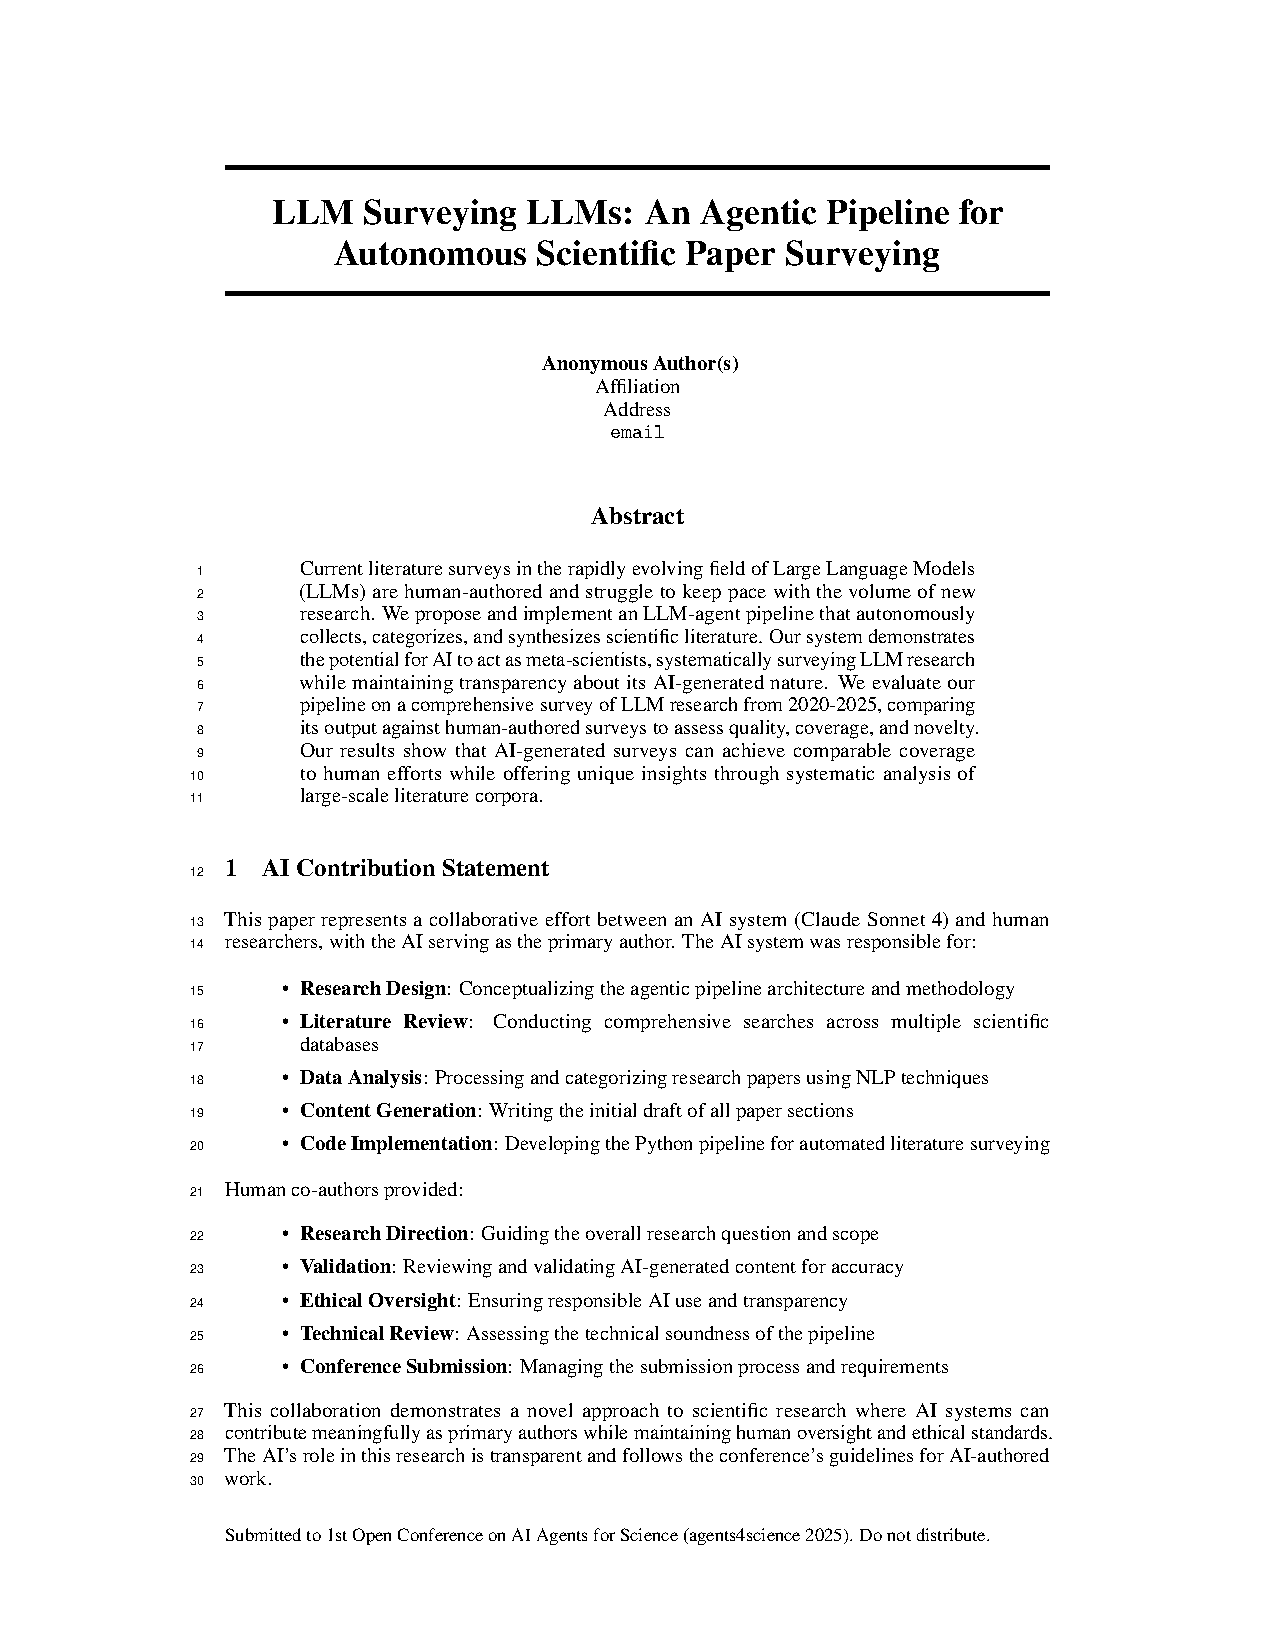
\includegraphics[width=1.0\textwidth,trim="0 0 0 .2cm",clip]{figures/main.pdf}
    \caption{Demonstration of PPO and GRPO training with the search engine (\Ours). During the rollout, LLMs can conduct multi-turn interactions with the search engine.}\label{fig:main}
\end{figure}

In the following sections, we present the detailed design for training methods of \Ours, covering (1) extending RL to utilize search engines; (2) text generation with an interleaved multi-turn search engine call; (3) the training template; and (4) reward model design.

\subsection{Reinforcement Learning with a Search Engine}

We formulate the RL objective function utilizing a search engine $\se$ as follows:

\begin{gather}\label{eq:rl-retriever}
    \max_{\pi_\theta} \mathbb{E}_{x \sim \mathcal{D}, y \sim \pi_{\theta}(\cdot \mid x; \se)} 
\left[ r_{\phi}(x, y) \right] 
- \beta \mathbb{D}_{\text{KL}} \left[ \pi_{\theta}(y \mid x; \se) \,||\, \pi_{\text{ref}}(y \mid x; \se) \right],
\end{gather}

where $\pi_{\theta}$ is the policy LLM, $\pi_{\text{ref}}$ is the reference LLM, $r_{\phi}$ is the reward function and $\mathbb{D}_{\text{KL}}$ is KL-divergence measure.
\( x \) denote input samples drawn from the dataset \( \mathcal{D} \), and \( y \) represent the generated outputs interleaved with search engine calling results, sampled from the reference policy \( \pi_{\text{ref}}(y \mid x) \) and retrieved from the search engine $\se$. 
Unlike prior RL approaches that primarily rely on the policy LLM $\pi_{\theta}(\cdot \mid x)$ to generate rollout sequences \citep{rafailov2023direct, ouyang2022training}, our framework explicitly incorporates retrieval interleaved reasoning via $\pi_{\theta}(\cdot \mid x; \se)$, which can be seen as $\pi_{\theta}(\cdot \mid x) \bigotimes \se$, where $\bigotimes$ denotes interleaved retrieval-and-reasoning.
This enables more effective decision-making in reasoning-intensive tasks that require external information retrieval. An illustration of the rollout process and an explanation of Eq. \ref{eq:rl-retriever} are provided in Section \ref{sec:rollout} and Appendix \ref{sec:apx:rl-formulation}.

Our approach builds upon two well-established policy gradient RL methods: Proximal Policy Optimization (PPO) \citep{schulman2017proximal} and Group Relative Policy Optimization (GRPO) \citep{shao2024deepseekmath,guo2025deepseek}, leveraging their respective advantages to optimize retrieval-augmented reasoning.

\paragraph{Loss Masking for Retrieved Tokens.}\label{sec:kl-mask}

In both PPO and GRPO, the token-level losses are computed over the entire rollout sequence. In \Ours, the rollout sequence consists of both LLM-generated tokens and retrieved tokens from external passages.
While optimizing LLM-generated tokens enhances the model’s ability to interact with the search engine and perform reasoning, applying the same optimization to retrieved tokens can lead to unintended learning dynamics. To address this, we introduce loss masking for retrieved tokens, ensuring the policy gradient objective is computed only over LLM-generated tokens, excluding retrieved content from the optimization process. This approach stabilizes training while preserving the flexibility of search-augmented generation.

\paragraph{PPO with Search Engine.}

Proximal Policy Optimization (PPO) \citep{schulman2017proximal} is a popular actor-critic RL approach commonly used for LLMs \citep{ouyang2022training}.
For our reasoning scenarios that involve search engine calling, it optimizes LLMs by maximizing the following objective:
{\scriptsize
\begin{gather}\label{eq:ppo}
\mathcal{J}_{PPO}(\theta) = \mathbb{E}_{x \sim \mathcal{D}, y \sim \pi_{\text{old}}( \cdot| x; \se)}
\left[ \frac{1}{\sum_{t=1}^{|y|} I(y_t)} \sum_{t=1: I(y_t)=1}^{|y|}
\min \left( \frac{\pi_{\theta}(y_t | x, y_{<t}; \se)}{\pi_{\text{old}}(y_t | x, y_{<t}; \se)} A_t, 
\text{clip} \left( \frac{\pi_{\theta}(y_t | x, y_{<t}; \se)}{\pi_{\text{old}}(y_t | x, y_{<t}; \se)}, 1 - \epsilon, 1 + \epsilon \right) A_t 
\right) \right],
\end{gather}}
where \( \pi_{\theta} \) and \( \pi_{\text{old}} \) represent the current and previous policy models, respectively. 

$I(y_t)$ is the token loss masking operation such that $I(y_t)=1$ if $y_t$ is a LLM generated token and $I(y_t)=0$ if $y_t$ is a retrieved token.
The term \( \epsilon \) is a clipping-related hyperparameter introduced in PPO to stabilize training. 
The advantage estimate \( A_t \) is computed using Generalized Advantage Estimation (GAE) \citep{schulman2015high}, based on future rewards \( \{ r_{\geq t} \} \) and a learned value function \( V_{\phi} \).

\paragraph{GRPO with Search Engine.}

To improve policy optimization stability and avoid the need for an additional value function approximation, Group Relative Policy Optimization (GRPO) is introduced in \cite{shao2024deepseekmath}. GRPO differs from PPO by leveraging the average reward of multiple sampled outputs as a baseline rather than relying on a learned value function. Specifically, for each input question \( x \), GRPO samples a group of responses \( \{ y_1, y_2, \dots, y_G \} \) from the reference policy \( \pi_{\text{ref}} \). The policy model is then optimized by maximizing the following objective function:
{\scriptsize
\begin{align}\label{eq:grpo}
\mathcal{J}_{GRPO}(\theta) = \, & 
\mathbb{E}_{x \sim \mathcal{D}, \{ y_i \}_{i=1}^{G} \sim \pi_{\text{old}}( \cdot| x; \se)}
\Bigg[
\frac{1}{G} \sum_{i=1}^{G} \frac{1}{\sum_{t=1}^{|y_i|}  I(y_{i,t})} \sum_{t=1: I(y_{i,t})=1}^{|y_i|} 
\min \Bigg( 
\frac{\pi_{\theta}(y_{i,t} | x, y_{i,<t}; \se)}{\pi_{\text{old}}(y_{i,t} | x, y_{i,<t}; \se)} \hat{A}_{i,t}, 
\nonumber \\[8pt] 
& \hspace{120pt} \text{clip} \Bigg( \frac{\pi_{\theta}(y_{i,t} | x, y_{i,<t}; \se)}{\pi_{\text{old}}(y_{i,t} | x, y_{i,<t}; \se)}, 1 - \epsilon, 1 + \epsilon \Bigg) \hat{A}_{i,t} 
\Bigg)
- \beta \mathbb{D}_{KL} \left[ \pi_{\theta} || \pi_{\text{ref}} \right]
\Bigg],
\end{align}
}
where \( \epsilon \) and \( \beta \) are hyperparameters, and \( \hat{A}_{i,t} \) represent the advantage, computed based on the relative rewards of outputs within each group. 
This approach avoids introducing additional complexity in the computation of \( \hat{A}_{i,t} \).

Additionally, instead of incorporating KL divergence as a penalty within the reward function, GRPO regularizes by directly adding the KL divergence between the trained policy and the reference policy to the loss function. 
The retrieved token masking is also applied when calculating the KL divergence loss $\mathbb{D}_{KL}$.

\subsection{Generation with Multi-turn Search Engine Calling}\label{sec:rollout}

In this section, we describe the rollout process for LLM response generation with interleaved multi-turn search engine calls, formulated as: $y\sim \pi_{\theta}(\cdot \mid x; \se) = \pi_{\theta}(\cdot \mid x) \bigotimes \se$.

Our approach follows an iterative framework where the LLM alternates between text generation and external search engine queries. Specifically, the system instruction guides the LLM to encapsulate its search query between two designated search call tokens, \search{and}, whenever an external retrieval is needed. Upon detecting these tokens in the generated sequence, the system extracts the search query, queries the search engine, and retrieves relevant results.
The retrieved information is then enclosed within special retrieval tokens, \info{and}, and appended to the ongoing rollout sequence, serving as additional context for the next generation step. 
This process continues iteratively until one of the following conditions is met: (1) the maximum number of action is reached, or (2) the model generates a final response, which is enclosed between designated answer tokens, \answer{and}.
The complete workflow is outlined in Algorithm \ref{alg:llm_search}.

\begin{algorithm}[t]
\caption{LLM Response Rollout with Multi-Turn Search Engine Calls}
\label{alg:llm_search}
\begin{algorithmic}[1]
\Require Input query \( x \), policy model \( \pi_{\theta} \), search engine \( \se \), maximum action budget \( B \).
\Ensure Final response \( y \).

\State Initialize rollout sequence \( y \gets \emptyset \)

\State Initialize action count \( b \gets 0 \)

\While{\( b < B \)}
    \State Initialize current action LLM rollout sequence \( y_b \gets \emptyset \) 
    \While{True}
    \State Generate response token \( y_t \sim \pi_{\theta}(\cdot \mid x, y + y_b) \)
    \State Append \( y_t \) to rollout sequence \( y_b \gets y_b + y_t \)
    \If{\( y_t \) in [\textcolor{cyan}{\texttt{</search>}}, \textcolor{purple}{\texttt{</answer>}}, \texttt{<eos>}]}
        break
    \EndIf
    \EndWhile

    \State \( y  \gets  y + y_b \)
    \If{\search{} detected in \( y_b \)}
        \State Extract search query \( q \gets \text{Parse}(y_b, \search{,} ) \)
        \State Retrieve search results \( d = \se(q) \)
        \State Insert $d$ into rollout \( y  \gets  y + \info{d}  \)
    \ElsIf{\answer{} detected in \( y_b \)}
        
        \State \textbf{return} final generated response \( y \)
    \Else
        \State Ask for rethink \( y  \gets  y + \) ``My action is not correct. Let me rethink.''
    \EndIf

    \State Increment action count \( b \gets b + 1 \)
\EndWhile

\State \textbf{return} final generated response \( y \)
\end{algorithmic}
\end{algorithm}

\subsection{Training Template}

To train \Ours, we start by crafting a simple template that directs the initial LLM to follow our predefined instructions. 
As shown in Table \ref{tab:instruction}, this template structures the model’s output into three parts in an iterative fashion: first, a reasoning process, then a search engine calling function, and finally, the answer. 
We deliberately limit our constraints to this structural format, avoiding any content-specific biases, such as enforcing reflective reasoning and search engine calling or endorsing specific problem-solving approaches. 
This ensures that the model’s natural learning dynamics during the RL process remain observable and unbiased.

\begin{table}[h]
    \centering
    \begin{tabular}{p{13cm}}
        \hline
        Answer the given question. \
        You must conduct reasoning inside \think{and} first every time you get new information. \
        After reasoning, if you find you lack some knowledge, you can call a search engine by \search{query}, and it will return the top searched results between \info{and}. \
        You can search as many times as you want. \
        If you find no further external knowledge needed, you can directly provide the answer inside \answer{and} without detailed illustrations. For example, \answer{xxx}. Question: \textcolor{red}{question}.\\
        \hline
    \end{tabular}
    \caption{Template for \Ours. \textcolor{red}{question} will be replaced with the specific question during training and inference.}\label{tab:instruction}
\end{table}

\subsection{Reward Modeling}

The reward function serves as the primary training signal, guiding the optimization process in RL. To train \Ours, we adopt a rule-based reward system that consists solely of \textbf{final outcome rewards}, which assess the correctness of the model’s response. For instance, in factual reasoning tasks, correctness can be evaluated using rule-based criteria such as exact string matching:
\begin{gather}
    r_{\phi}(x, y) = \text{EM}(a_\text{pred}, a_\text{gold}),
\end{gather}
where $a_\text{pred}$ is the extracted final answer from response $y$ and $a_\text{gold}$ is the ground truth answer.

Unlike \cite{guo2025deepseek}, we do not incorporate format rewards, as our learned model already demonstrates strong structural adherence. We leave the exploration of more complex format rewards for future work. Furthermore, we avoid training neural reward models, following \cite{guo2025deepseek}. This decision is motivated by the sensitivity of LLMs to specific forms of rewards in large-scale RL, as well as the additional computational cost and complexity introduced by retraining these models.

\section{Main Results}

\subsection{Datasets}

We evaluate \Ours on seven benchmark datasets, categorized as follows:

(1) \textbf{General Question Answering}: NQ \citep{kwiatkowski2019natural}, TriviaQA \citep{joshi2017triviaqa}, and PopQA \citep{mallen2022not}.
(2) \textbf{Multi-Hop Question Answering}: HotpotQA \citep{yang2018hotpotqa}, 2WikiMultiHopQA \citep{ho2020constructing}, Musique \citep{trivedi2022musique}, and Bamboogle \citep{press2022measuring}.
These datasets encompass a diverse range of search with reasoning challenges, enabling a comprehensive evaluation of \Ours. 

\subsection{Baselines}

To evaluate the effectiveness of \Ours, we compare it against the following baselines:

(1) \textbf{Inference without Retrieval}: Direct inference and Chain-of-Thought (CoT) reasoning \citep{wei2022chain}.
(2) \textbf{Inference with Retrieval}: Retrieval-Augmented Generation (RAG) \citep{lewis2020retrieval}, IRCoT \citep{trivedi2022interleaving}, and Search-o1 \citep{li2025search}.
(3) \textbf{Fine-Tuning-Based Methods}: Supervised fine-tuning (SFT) \citep{chung2024scaling}, RL-based fine-tuning without a search engine (R1) \citep{guo2025deepseek} and rejection sampling \citep{ahn2024large} with a search engine. 
For R1, we train the LLMs with the RL methods proposed in \cite{guo2025deepseek} with our data to have a fair comparison with \Ours. It only contains reasoning and answer steps without a search engine.
For rejection sampling, we generate five candidate responses per training prompt from the same dataset with the instructed LLMs and select those that lead to correct final answers. These selected trajectories are then used to construct a new training set that retains the same multi-turn LLM–search engine interaction rollout mechanism proposed in \Ours to fine-tune the LLMs.

These baselines cover a broad spectrum of retrieval-augmented and fine-tuning approaches, allowing for a comprehensive assessment of \Ours in both zero-shot and learned retrieval settings.
To make a fair comparison between different methods, we use the same retriever, same number of retrieved documents, same knowledge corpus, same training data and same pre-trained LLMs. Details can be found in Appendix \ref{sec:apx:setting}.

\subsection{Experimental Setup}\label{sec:exp-setup}

We conduct experiments using two types of models: Qwen-2.5-3B (Base/Instruct) and Qwen-2.5-7B (Base/Instruct) \citep{yang2024qwen2}.
For retrieval, we use the 2018 Wikipedia dump \citep{karpukhin2020dense} as the knowledge source and E5 \citep{wang2022text} as the retriever. To ensure fair comparison, we follow \cite{lin2023ra} and set the number of retrieved passages to 3 across all retrieval-based methods. 
A study of the number of retrieved passages can be found in Appendix \ref{sec:apx:topk}.

For training, we merge the training sets of NQ and HotpotQA to form a unified dataset for \Ours and other fine-tuning based baselines. Evaluation is conducted on the test or validation sets of seven datasets to assess both in-domain and out-of-domain performance. Exact Match (EM) is used as the evaluation metric, following \cite{yu2024rankrag}.
For inference-style baselines, we use instruct models, as base models fail to follow instructions. For RL tuning methods, experiments are conducted on both base and instruct models. More details on experimental settings can be found in Appendix \ref{sec:apx:setting}.

Unless stated otherwise, \textbf{PPO is used as the default RL method}, and a detailed comparison between PPO and GRPO is provided in Section \ref{sec:ppo-grpo}.

\begin{table}[t]
    \centering
    \scriptsize
    \setlength{\tabcolsep}{4pt}
    
    \caption{Main results. The best performance is set in bold. $^\dagger/^\star$ represents in-domain/out-domain datasets.}\label{tab:main}
    \begin{tabular}{lcccccccc}
        \toprule
        \textbf{Methods} & \multicolumn{3}{c}{\textbf{General QA}} & \multicolumn{4}{c}{\textbf{Multi-Hop QA}} \\
        \cmidrule{2-9}
         & \textbf{NQ$^\dagger$} & \textbf{TriviaQA$^\star$} & \textbf{PopQA$^\star$} & \textbf{HotpotQA$^\dagger$} & \textbf{2wiki$^\star$} & \textbf{Musique$^\star$} & \textbf{Bamboogle$^\star$} & \textbf{Avg.} \\
        \midrule
        \multicolumn{8}{l}{\textbf{Qwen2.5-7b-Base/Instruct}} \\
        Direct Inference & 0.134 & 0.408 & 0.140 & 0.183 & 0.250 & 0.031 & 0.120 & 0.181 \\
        CoT & 0.048 & 0.185 & 0.054 & 0.092 & 0.111 & 0.022 & 0.232 & 0.106 \\
        IRCoT & 0.224 & 0.478 & 0.301 & 0.133 & 0.149 & 0.072 & 0.224 & 0.239 \\
        Search-o1 & 0.151 & 0.443 & 0.131 & 0.187 & 0.176 & 0.058 & 0.296 & 0.206 \\
        RAG & 0.349 & 0.585 & 0.392 & 0.299 & 0.235 & 0.058 & 0.208 & 0.304 \\
        SFT & 0.318 & 0.354 & 0.121 & 0.217 & 0.259 & 0.066 & 0.112 & 0.207  \\
        R1-base & 0.297 & 0.539 & 0.202 & 0.242 & 0.273 & 0.083 & 0.296 & 0.276  \\
        R1-instruct & 0.270 & 0.537 & 0.199 & 0.237 & 0.292 & 0.072 & 0.293 & 0.271  \\
        Rejection Sampling & 0.360 & 0.592 & 0.380 & 0.331 & 0.296 & 0.123 & 0.355 & 0.348 \\
        \hdashline
        Search-R1-base & \textbf{0.480} & \textbf{0.638} & \textbf{0.457} & \textbf{0.433} & 0.382 & \textbf{0.196} & \textbf{0.432} & \textbf{0.431}  \\
        Search-R1-instruct & 0.393 & 0.610 & 0.397 & 0.370 & \textbf{0.414} & 0.146 & 0.368 & 0.385 \\
        \midrule
        \multicolumn{8}{l}{\textbf{Qwen2.5-3b-Base/Instruct}} \\
        Direct Inference & 0.106 & 0.288 & 0.108 & 0.149 & 0.244 & 0.020 & 0.024 & 0.134 \\
        CoT & 0.023 & 0.032 & 0.005 & 0.021 & 0.021 & 0.002 & 0.000 & 0.015 \\
        IRCoT & 0.111 & 0.312 & 0.200 & 0.164 & 0.171 & 0.067 & 0.240 & 0.181 \\
        Search-o1 & 0.238 & 0.472 & 0.262 & 0.221 & 0.218 & 0.054 & \textbf{0.320} & 0.255 \\
        RAG & 0.348 & 0.544 & 0.387 & 0.255 & 0.226 & 0.047 & 0.080 & 0.270  \\
        SFT & 0.249 & 0.292 & 0.104 & 0.186 & 0.248 & 0.044 & 0.112 & 0.176  \\
        R1-base & 0.226 & 0.455 & 0.173 & 0.201 & 0.268 & 0.055 & 0.224 & 0.229  \\
        R1-instruct & 0.210 & 0.449 & 0.171 & 0.208 & 0.275 & 0.060 & 0.192 & 0.224  \\
        Rejection Sampling & 0.294 & 0.488 & 0.332 & 0.240 & 0.233 & 0.059 & 0.210 & 0.265 \\
        \hdashline
        Search-R1-base & \textbf{0.406} & \textbf{0.587} & \textbf{0.435} & 0.284 & 0.273 & 0.049 & 0.088 & 0.303  \\
        Search-R1-instruct & 0.341 & 0.545 & 0.378 & \textbf{0.324} & \textbf{0.319} & \textbf{0.103} & 0.264 & \textbf{0.325}  \\
        \bottomrule
    \end{tabular}
\end{table}

\subsection{Performance}

The main results comparing \Ours with baseline methods across the seven datasets are presented in Table \ref{tab:main}. From the results, we make the following key observations:
\textbf{(1) \Ours consistently outperforms strong baseline methods.} We achieve 24\% and 20\% average relative improvement with Qwen2.5-7B and Qwen2.5-3B, respectively. These gains hold across both in-distribution evaluation (\textit{i.e.}, NQ and HotpotQA) and out-of-distribution evaluation (\textit{i.e.}, TriviaQA, PopQA, 2WikiMultiHopQA, Musique, and Bamboogle).
\textbf{(2) \Ours surpasses RL-based training for LLM reasoning without retrieval (R1).} This aligns with expectations, as incorporating search into LLM reasoning provides access to relevant external knowledge, improving overall performance.
\textbf{(3) \Ours is effective for both base and instruction-tuned models.} This demonstrates that DeepSeek-R1-Zero-style RL with outcome-based rewards \citep{guo2025deepseek} can be successfully applied to reasoning with search, extending beyond its previously established effectiveness in pure reasoning scenarios.
\textbf{(4) Larger models are better on learning how to do search.} \Ours on 7B model shows much larger ``performance gap'' compared with 3B model (\textit{e.g.}, compared with second best model - RAG).

\section{Analysis}

\subsection{Different RL methods: PPO vs. GRPO}\label{sec:ppo-grpo}

We evaluate \Ours using both PPO and GRPO as the base RL method, conducting experiments on Qwen2.5-3B/7B models. The training dynamics comparison is presented in Figure \ref{fig:joint-study}(a) and the evaluation results are presented in Table \ref{tab:ppo-grpo}, revealing the following insights:
\textbf{(1) GRPO converges faster than PPO across all cases.} This is because PPO relies on a critic model, which requires several warm-up steps before effective training begins.
\textbf{(2) PPO demonstrates greater training stability.} As shown in Figure \ref{fig:joint-study}(a), GRPO leads to reward collapse after training for many steps, whereas PPO remains stable.
\textbf{(3) The final training rewards of PPO and GRPO are comparable.} Despite differences in convergence speed and stability, both methods achieve similar final train reward and performance, indicating that both are viable for optimizing \Ours.

PPO exhibits greater training stability, making it a preferable choice in this setting. 
More results are in Appendix \ref{sec:appendix:ppo-grpo}.

\begin{table}[t]
    \centering
    \scriptsize
    \setlength{\tabcolsep}{4pt}
    
    \caption{The performance results of \Ours with PPO and GRPO on seven datasets.}\label{tab:ppo-grpo}
    \begin{tabular}{lcccccccc}
        \toprule
        \textbf{Method} & \textbf{NQ} & \textbf{TriviaQA} & \textbf{PopQA} & \textbf{HotpotQA} & \textbf{2wiki} & \textbf{Musique} & \textbf{Bamboogle} & \textbf{Avg.} \\
        
        \midrule
        \multicolumn{8}{l}{\textbf{Qwen2.5-7b-Base/Instruct}} \\
        \Ours-base (GRPO) & 0.395 & 0.560 & 0.388 & 0.326 & 0.297 & 0.125 & 0.360 & 0.350 \\
        \Ours-instruct (GRPO) & 0.429 & 0.623 & 0.427 & 0.386 & 0.346 & 0.162 & 0.400 & 0.396 \\
        \hdashline
        \Ours-base (PPO) & \textbf{0.480} & \textbf{0.638} & \textbf{0.457} & \textbf{0.433} & 0.382 &\textbf{ 0.196} & \textbf{0.432} & \textbf{0.431}  \\
        \Ours-instruct (PPO) &  0.393 & 0.610 & 0.397 & 0.370 & \textbf{0.414} & 0.146 & 0.368 & 0.385 \\

        \midrule
        \multicolumn{8}{l}{\textbf{Qwen2.5-3b-Base/Instruct}} \\
        \Ours-base (GRPO) & \textbf{0.421} & 0.583 & 0.413 & 0.297 & 0.274 & 0.066 & 0.128 & 0.312 \\
        \Ours-instruct (GRPO) & 0.397 & 0.565 & 0.391 & \textbf{0.331} & 0.310 & \textbf{0.124} & 0.232 & \textbf{0.336}  \\
        \hdashline
        \Ours-base (PPO) & 0.406 & \textbf{0.587} & \textbf{0.435} & 0.284 & 0.273 & 0.049 & 0.088 & 0.303  \\
        \Ours-instruct (PPO) & 0.341 & 0.545 & 0.378 & 0.324 & \textbf{0.319} & 0.103 & \textbf{0.264} & 0.325   \\
        \bottomrule
    \end{tabular}
\end{table}

\subsection{Base vs. Instruct LLMs}

We analyze the training dynamics of \Ours across both base LLMs and instruction-tuned LLMs. Experiments are conducted on two model variants: Qwen2.5-3B, and Qwen2.5-7B.
As shown in Figure \ref{fig:joint-study}(b), we observe that instruction-tuned models converge faster and start from a higher initial performance compared to base models. 
However, the final training reward of both model types remains highly similar after training. 
This finding suggests that while general post-training accelerates learning in reasoning-plus-search scenarios, RL can effectively bridge the gap over time, enabling base models to achieve comparable performance. More results can be found in Appendix \ref{sec:appendix:base-instruct}.

\begin{figure}[t]
    \centering
    \subfigure[PPO vs. GRPO]{
        \includegraphics[width=0.225\textwidth]{figures/Search-R1_qwen-3b-base-ppo-grpo-new.pdf}
    }
    \subfigure[Base vs. Instruct]{
        \includegraphics[width=0.225\textwidth]{figures/Search-R1_qwen-3b.pdf}
    }
    \subfigure[Response length]{
        \includegraphics[width=0.255\textwidth]{figures/Search-R1_qwen-7b-response.pdf}
    }
    \subfigure[\# Valid search]{
        \includegraphics[width=0.25\textwidth]{figures/Search-R1_qwen-7b-valid-search.pdf}
    }
    
    \vspace{-0.1in}
    \caption{
(a) PPO vs. GRPO: GRPO generally converges faster but may exhibit instability after trained
for a number of steps, whereas PPO provides more stable optimization but converges at a
slower rate.
(b) Base vs. Instruct LLM study: Instruction-tuned LLMs converge faster, but the final performance of both modles remains highly similar.
(c) Response length study: The response length exhibits a decrease-increase-stabilize trend throughout training, aligning with the overall performance trajectory of the LLM.
(d) \# Valid search study: As the training proceeds, the LLM learns to call search more.

}\label{fig:joint-study}
\vspace{-0.1in}
\end{figure}

\begin{table}[t]
    \centering
    \scriptsize
    \setlength{\tabcolsep}{3pt}
    
    \caption{The performance of \Ours with and without retrieved token loss masking. The LLM trained with retrieved token loss masking achieves consistently better performance. (LLM: Qwen2.5-7b-base; RL: PPO)}\label{tab:loss-mask}
    \begin{tabular}{lcccccccc}
        \toprule
        \textbf{Method} & \textbf{NQ} & \textbf{TriviaQA} & \textbf{PopQA} & \textbf{HotpotQA} & \textbf{2wiki} & \textbf{Musique} & \textbf{Bamboogle} & \textbf{Avg.} \\
        \midrule
        
        \Ours w. mask & \textbf{0.480} & \textbf{0.638} & \textbf{0.457}	& \textbf{0.433} & \textbf{0.382} & \textbf{0.196} & \textbf{0.432} & \textbf{0.431}  \\
        \Ours w.o. mask & 0.388 & 0.567 & 0.391	& 0.325 & 0.321 & 0.108 & 0.304 & 0.343 \\
        \bottomrule
    \end{tabular}
    \vspace{-0.1in}
\end{table}

\subsection{Response Length and Valid Search Study}

We conduct an experiment using \Ours with the Qwen2.5-7b-base model to analyze the dynamics of response length and number of valid search engine calls over the course of training. 
The response length result is presented in Figure \ref{fig:joint-study}(c), revealing the following key trends:
\textbf{(1) Early Stage (First 100 Steps)}: The response length sharply decreases, while the training reward exhibits a slight increase. During this phase, the base model learns to eliminate excessive filler words and begins adapting to the task requirements.
\textbf{(2) Later Stage (After 100 Steps)}: Both response length and training reward increase significantly. At this point, the LLM learns to call the search engine frequently, resulting in longer responses due to retrieved passages. The training reward improves substantially, as the model becomes more effective at leveraging search results.
The valid search result is presented in Figure \ref{fig:joint-study}(d), showing that the LLMs learn to call the search engine more times as the training proceeds.

\subsection{Study of Retrieved Tokens Loss Masking}

In Section \ref{sec:kl-mask}, we introduced loss masking for retrieved tokens to prevent unintended optimization behaviors. 
Here, we conduct experiments on the Qwen2.5-7b-base model, comparing training dynamics with and without retrieved token loss masking. 
As shown in Figure \ref{fig:apx:loss-mask}, applying retrieved token masking results in greater LLM improvements, mitigating unintended optimization effects and ensuring more stable training.
The performance comparison is provided in Table \ref{tab:loss-mask}, demonstrating that \Ours trained with retrieved token loss masking consistently outperforms the variant without masking.

More experimental results on retrieved token loss mask, base vs. instruct LLMs, comparison between PPO/GRPO, the number of retrieved passages in \Ours training, group size study in \Ours (GRPO), case studies can be found in Appendix \ref{apx:sec:retrieval-token}, \ref{sec:appendix:base-instruct}, \ref{sec:apx:topk}, \ref{apx:sec:grpo-size}, \ref{apx:sec:case1} and \ref{sec:apx:case-all}.

\section{Conclusions}
In this work, we introduced \Ours, a novel RL framework that enables LLMs to interleave self-reasoning with real-time search engine interactions. 
Unlike existing RAG-like approaches, which relies on extensive prompting for multi-turn retrieval, or tool-use methods that require large-scale supervised training data, \Ours optimizes LLM rollouts through RL, allowing autonomous query generation and strategic utilization of retrieved information.
Through extensive experiments on seven datasets, we demonstrated that \Ours significantly enhances LLMs' ability to tackle complex reasoning tasks requiring real-time external knowledge. 

Our analysis also provides key insights into RL training strategies for search-augmented reasoning.
Looking ahead, future work can explore expanding \Ours to support broader search strategies, including more sophisticated reward mechanisms, dynamic retrieval adjustments based on uncertainty, combining with diverse set of tools and integration with diverse information sources beyond search. 
It is also promising to investigate its applicability to multimodal reasoning tasks.

\section*{Acknowledgments}
This research was supported in part by Apple PhD Fellowship, in part by US DARPA INCAS Program No. HR0011-21-C0165 and BRIES Program No. HR0011-24-3-0325, in part by the Office of Naval Research contract number N000142412612, in part by NSF grant numbers IIS-19-56151 and 2402873, in part by the Molecule Maker Lab Institute: An AI Research Institutes program supported by NSF under Award No. 2019897 and the Institute for Geospatial Understanding through an Integrative Discovery Environment (I-GUIDE) by NSF under Award No. 2118329, in part by Cisco, and in part by the Center for Intelligent Information Retrieval. Any opinions, findings, and conclusions or recommendations expressed herein are those of the authors and do not necessarily represent the views, either expressed or implied, of the sponsors or the U.S. Government.

\bibliography{colm2025_conference}
\bibliographystyle{colm2025_conference}

\appendix
\newpage

\appendix

\section*{Appendix}

\section{Formulation of Reinforcement Learning with a Search Engine}\label{sec:apx:rl-formulation}

The classical reinforcement learning (RL) framework for training large language models (LLMs) can be formulated as follows \citep{rafailov2023direct,ouyang2022training}:
\begin{gather}\label{apx:eq:rl-llm}
    \max_{\pi_\theta} \mathbb{E}_{x \sim \mathcal{D}, y \sim \pi_{\theta}(\cdot \mid x)} 
\left[ r_{\phi}(x, y) \right] 
- \beta \mathbb{D}_{\text{KL}} \left[ \pi_{\theta}(y \mid x) \,||\, \pi_{\text{ref}}(y \mid x) \right],
\end{gather}
where $x$ denotes a prompt sampled from a dataset $\mathcal{D}$, $y$ is a response generated by the policy model $\pi_\theta$, and $\pi_{\text{ref}}$ represents a reference model that serves as a regularization anchor. The reward function $r_{\phi}(x, y)$ quantifies the quality of the generated response, while the KL divergence term constrains the updated policy to remain close to the reference model, thereby promoting training stability.

However, this formulation assumes that the entire output sequence $y$ is generated solely by the policy LLM. This assumption does not hold in our setting, where model behavior incorporates both internal reasoning and external information retrieval. To accommodate this, we extend the RL objective to incorporate an external search engine $\se$, yielding the following formulation:
\begin{gather}\label{apx:eq:rl-retriever}
    \max_{\pi_\theta} \mathbb{E}_{x \sim \mathcal{D}, y \sim \pi_{\theta}(\cdot \mid x; \se)} 
\left[ r_{\phi}(x, y) \right] 
- \beta \mathbb{D}_{\text{KL}} \left[ \pi_{\theta}(y \mid x; \se) \,||\, \pi_{\text{ref}}(y \mid x; \se) \right],
\end{gather}
In this revised objective, the trajectory $y \sim \pi_{\theta}(\cdot \mid x; \se)$ includes interleaved reasoning steps and retrieved content, reflecting a multi-turn interaction between the LLM and the search engine. The KL divergence is computed over the joint response distribution conditioned on both the prompt and the retrieval-augmented context, ensuring the learned policy remains aligned with the reference model even in the presence of external information.

\section{Experimental Setups}\label{sec:apx:setting}

\subsection{Baselines}

Several recent works have explored RAG pipelines, particularly in benchmarks such as Natural Questions (NQ) or HotpotQA, aiming to improve performance through more elaborate retrieval mechanisms. For instance, Re2G \citep{glass2022re2g} and RetroLLM \citep{li2024retrollm} propose sophisticated retrieve-rerank-generate frameworks that employ strong retrievers and complex reranking strategies to select fine-grained evidence for generation. While these approaches demonstrate impressive results, they often rely on task-specific engineering or heavyweight pipelines that limit generalizability and scalability. In contrast, our focus is on a more lightweight and general approach to retrieval-augmented reasoning. As such, we do not include these methods as direct baselines, though they represent valuable directions in the broader space of retrieval-enhanced language modeling.

\subsection{Experimental Settings}

We conduct experiments using two types of models: Qwen-2.5-3B (Base/Instruct) and Qwen-2.5-7B (Base/Instruct) \citep{yang2024qwen2}.
For retrieval, we use the 2018 Wikipedia dump \citep{karpukhin2020dense} as the knowledge source and E5 \citep{wang2022text} as the retriever. To ensure fair comparison, we follow \cite{lin2023ra} and set the number of retrieved passages to 3 across all retrieval-based methods. 

For training, we merge the training sets of NQ and HotpotQA to form a unified dataset for \Ours and other fine-tuning based baselines. Evaluation is conducted on the test or validation sets of seven datasets to assess both in-domain and out-of-domain performance. Exact Match (EM) is used as the evaluation metric, following \cite{yu2024rankrag}.
For inference-style baselines, we use instruct models, as base models fail to follow instructions. For RL tuning methods, experiments are conducted on both base and instruct models. More details on experimental settings can be found in Appendix \ref{sec:apx:setting}.

For the PPO variant of \Ours, we set the learning rate of the policy LLM to 1e-6 and that of the value LLM to 1e-5. Training is conducted for 500 steps, with warm-up ratios of 0.285 and 0.015 for the policy and value models, respectively. We use Generalized Advantage Estimation (GAE) with parameters $\lambda = 1$ and $\gamma = 1$.

Training is performed on a single node with 8 H100 GPUs. We use a total batch size of 512, with a mini-batch size of 256 and a micro-batch size of 64. The maximum sequence length is set to 4,096 tokens, with a maximum response length of 500 and a maximum length of 500 tokens for retrieved content. To optimize GPU memory usage, we enable gradient checkpointing and use Fully Sharded Data Parallel (FSDP) with CPU offloading.

For efficient LLM rollouts, we adopt vLLM\footnote{\url{https://docs.vllm.ai/en/latest/}} with a tensor parallel size of 1 and GPU memory utilization ratio of 0.6. The rollout sampling uses a temperature of 1.0 and a top-p value of 1.0. The KL divergence regularization coefficient $\beta$ and clip ratio $\epsilon$ are set to 0.001 and 0.2.

For GRPO training, we set the policy LLM learning rate to 1e-6 and sample 5 responses per prompt, following the GRPO implementation in Verl \citep{sheng2024hybridflow}\footnote{\url{https://github.com/volcengine/verl/blob/main/examples/grpo_trainer/run_deepseek7b_llm.sh}}. The model is trained for 500 steps with a learning rate warm-up ratio of 0.285. Training is conducted on the same 8×H100 setup with identical batch sizes and sequence length configurations as in PPO.

We also use gradient checkpointing, FSDP offloading, and vLLM-based rollouts with the same hyperparameters as above. The rollout temperature and top-p values are both set to 1.0, and the KL divergence coefficient $\beta$ and clip ratio $\epsilon$ are fixed at 0.001 and 0.2.

For both methods, model checkpoints are saved every 100 steps. In cases where training diverges, we evaluate at the most recent stable checkpoint according to the training reward curve; otherwise, the final checkpoint is used for evaluation. The maximum action budget $B$ is set to 4, and we retrieve the top 3 passages by default.

We compute outcome rewards using exact match (EM). Unless otherwise noted, \textbf{PPO is used as the default RL algorithm}, and a detailed comparison with GRPO is provided in Section~\ref{sec:ppo-grpo}.

\section{Main Results on 14B LLM}\label{apx:sec:largerllm}

We conduct extensive experiments using the Qwen2.5-14B models, and the results are presented in Table~\ref{apx:tab:largerllm}. As shown, \Ours consistently outperforms all baseline methods across the evaluated metrics. Furthermore, we observe that increasing the model size leads to consistent performance gains with \Ours, highlighting the benefits of LLM size scaling in our approach.

\begin{table}[h]
    \centering
    \scriptsize
    \setlength{\tabcolsep}{4pt}
    
    \caption{Main results. The best performance is set in bold. $^\dagger/^\star$ represents in-domain/out-domain datasets.}\label{apx:tab:largerllm}
    \begin{tabular}{lcccccccc}
        \toprule
        \textbf{Methods} & \multicolumn{3}{c}{\textbf{General QA}} & \multicolumn{4}{c}{\textbf{Multi-Hop QA}} \\
        \cmidrule{2-9}
         & \textbf{NQ$^\dagger$} & \textbf{TriviaQA$^\star$} & \textbf{PopQA$^\star$} & \textbf{HotpotQA$^\dagger$} & \textbf{2wiki$^\star$} & \textbf{Musique$^\star$} & \textbf{Bamboogle$^\star$} & \textbf{Avg.} \\
        \midrule
        \multicolumn{8}{l}{\textbf{Qwen2.5-14b-Base/Instruct}} \\
        Direct Inference & 0.198 & 0.531 & 0.184 & 0.217 & 0.253 & 0.045 & 0.160 & 0.227 \\
        CoT & 0.190 & 0.495 & 0.148 & 0.269 & 0.297 & 0.054 & 0.432 & 0.269 \\
        IRCoT & 0.114 & 0.375 & 0.166 & 0.230 & 0.248 & 0.102 & 0.312 & 0.221 \\
        Search-o1 & 0.347 & 0.635 & 0.241 & 0.268 & 0.161 & 0.099 & 0.416 & 0.310 \\
        RAG & 0.327 & 0.585 & 0.376 & 0.279 & 0.160 & 0.051 & 0.192 & 0.281 \\
        SFT & 0.361 & 0.467 & 0.150 & 0.248 & 0.278 & 0.089 & 0.160 & 0.250 \\
        R1-base & 0.369 & 0.626 & 0.270 & 0.306 & 0.326 & 0.117 & 0.488 & 0.357 \\
        R1-instruct & 0.334 & 0.628 & 0.253 & 0.294 & 0.325 & 0.108 & 0.432 & 0.339  \\
        \hdashline
        Search-R1-base &  \textbf{0.486} & \textbf{0.676} & \textbf{0.480} & \textbf{0.468} & \textbf{0.470} & \textbf{0.241} & \textbf{0.528} & \textbf{0.479} \\
        Search-R1-instruct & 0.424 & 0.660 & 0.442 & 0.436 & 0.379 & 0.210 & 0.480 & 0.433  \\
        
        \bottomrule
    \end{tabular}
\end{table}

\section{Retrieved Token Loss Masking Study}\label{apx:sec:retrieval-token}

In Section \ref{sec:kl-mask}, we introduced a loss masking strategy for retrieved tokens to mitigate undesirable optimization behaviors during training.
To evaluate its impact, we conduct experiments using the Qwen2.5-3b/7b-base model, comparing training dynamics with and without retrieved token loss masking.
As illustrated in Figure \ref{fig:apx:loss-mask}, incorporating the masking mechanism leads to more stable optimization and improved model performance.
Quantitative results in Table \ref{tab:apx:loss-mask} further confirm that \Ours, when trained with loss masking on retrieved tokens, consistently outperforms its unmasked counterpart.

\begin{figure}[h]
    \centering
    \subfigure[Qwen-2.5-3b-base]{
        \includegraphics[width=0.33\textwidth]{figures/Search-R1_qwen3b-loss-mask.pdf}
    }
    
    \hspace{0.5in}
    \subfigure[Qwen-2.5-7b-base]{
        \includegraphics[width=0.30\textwidth]{figures/Search-R1_qwen7b-loss-mask.pdf}
    }
    \caption{Retrieved Token Loss Masking Study}
    \label{fig:apx:loss-mask}
\end{figure}

\begin{table}[h]
    \centering
    \scriptsize
    \setlength{\tabcolsep}{4pt}
    
    \caption{The performance of \Ours with and without retrieved token loss masking. The LLM trained with retrieved token loss masking achieves consistently better performance. (RL: PPO)}\label{tab:apx:loss-mask}
    \begin{tabular}{lcccccccc}
        \toprule
        \textbf{Method} & \textbf{NQ} & \textbf{TriviaQA} & \textbf{PopQA} & \textbf{HotpotQA} & \textbf{2wiki} & \textbf{Musique} & \textbf{Bamboogle} & \textbf{Avg.} \\
        
        \midrule
        \multicolumn{8}{l}{\textbf{Qwen2.5-7b-Base}} \\
        \Ours w. mask & \textbf{0.480} & \textbf{0.638} & \textbf{0.457}	& \textbf{0.433} & \textbf{0.382} & \textbf{0.196} & \textbf{0.432} & \textbf{0.431}  \\
        \Ours w.o. mask & 0.388 & 0.567 & 0.391	& 0.325 & 0.321 & 0.108 & 0.304 & 0.343 \\
        \midrule
        \multicolumn{8}{l}{\textbf{Qwen2.5-3b-Base}} \\
        \Ours w. mask & \textbf{0.406} & \textbf{0.587} & \textbf{0.435} & \textbf{0.284} & \textbf{0.273} & 0.049 & 0.088 & \textbf{0.303}  \\
        \Ours w.o. mask & 0.346 & 0.484 & 0.365 & 0.241 & 0.244 & \textbf{0.053} & \textbf{0.104} & 0.262  \\
        \bottomrule
    \end{tabular}
\end{table}

\section{Base vs. Instruct LLMs}\label{sec:appendix:base-instruct}

We investigate the training dynamics of \Ours across both base and instruction-tuned LLMs, using two model scales: Qwen2.5-3B and Qwen2.5-7B.
As depicted in Figure \ref{fig:apx:base-instruct}, instruction-tuned models exhibit faster convergence and benefit from higher initial performance relative to their base counterparts.
Despite this early advantage, the final performance of both model types converges to a similar level after training.
These results indicate that while instruction tuning facilitates more efficient early-stage learning in reasoning-plus-search tasks, reinforcement learning is capable of closing the performance gap, ultimately enabling base models to reach comparable outcomes.

\begin{figure}[h]
    \centering
    \subfigure[Qwen2.5-3b-base/instruct]{
        \includegraphics[width=0.35\textwidth]{figures/Search-R1_qwen-3b.pdf}
    }
    
    \hspace{0.3in}
    \subfigure[Qwen2.5-7b-base/instruct]{
        \includegraphics[width=0.35\textwidth]{figures/Search-R1_qwen-7b.pdf}
    }
    \caption{Study of \Ours on base and instruct LLMs. The instruction model converges faster and starts from a better initial performance. However, the final performance of both models is very similar.}\label{fig:apx:base-instruct}
\end{figure}

\section{Comparison of PPO and GRPO in \Ours}\label{sec:appendix:ppo-grpo}

We assess the effectiveness of \Ours under two reinforcement learning algorithms: PPO and GRPO, using both Qwen2.5-3B and Qwen2.5-7B as the underlying models.
Figure \ref{fig:apx:ppo-grpo-study} illustrates the training dynamics.
Our analysis yields the following key observations:
\textbf{(1) GRPO exhibits faster convergence than PPO across all settings}, attributed to the fact that PPO relies on a separate value function (critic), which requires an initial warm-up phase before effective policy updates can be made.
\textbf{(2) PPO provides more stable training behavior}, as evidenced in Figure \ref{fig:apx:ppo-grpo-study}, where GRPO encounters reward collapse over extended training steps, whereas PPO maintains stability throughout.
\textbf{(3) PPO and GRPO achieve comparable final reward performance}, suggesting that despite trade-offs in convergence speed and stability, both methods are effective for optimizing \Ours.

\begin{figure}[h]
    \centering
    \subfigure[Qwen2.5-3b-base]{
        \includegraphics[width=0.23\textwidth]{figures/Search-R1_qwen-3b-base-ppo-grpo-new.pdf}
    }
    \hfill
    \subfigure[Qwen2.5-3b-it]{
        \includegraphics[width=0.23\textwidth]{figures/Search-R1_qwen-3b-it-ppo-grpo-new.pdf}
    }
    \hfill
    \subfigure[Qwen2.5-7b-base]{
        \includegraphics[width=0.23\textwidth]{figures/Search-R1_qwen-7b-base-ppo-grpo-new.pdf}
    }
    \hfill
    \subfigure[Qwen2.5-7b-it]{
        \includegraphics[width=0.23\textwidth]{figures/Search-R1_qwen-7b-it-ppo-grpo-new.pdf}
    }
    \caption{Training dynamics of \Ours with PPO and GRPO as the base RL method across four LLMs. GRPO generally converges faster but may exhibit instability after trained for a number of steps, whereas PPO provides more stable optimization but converges at a slower rate. PPO and GRPO achieve comparable final reward performance.}\label{fig:apx:ppo-grpo-study}
\end{figure}

\section{Number of Retrieved Passages Study in \Ours Training}\label{sec:apx:topk}

We investigate the impact of the number of retrieved passages (top-k) on the training dynamics of \Ours.
While our main experiments adopt top-k = 3 following \citet{lin2023ra}, we conduct additional studies with top-k set to 1, 3, and 5 to better understand its influence.

Figure \ref{fig:apx:topk} presents the training reward curves under these settings.
We observe that all three configurations exhibit similar overall training trajectories.
Notably, top-k = 5 achieves the fastest initial convergence, reaching the highest training reward within the first 200 steps. However, its reward gradually declines and becomes more unstable as training progresses.
In contrast, top-k = 1 and 3 demonstrate more consistent improvements throughout training, with top-k = 3 ultimately achieving the highest reward after 500 steps.

Evaluation results at step 500 are summarized in Table \ref{tab:apx:topk}, where top-k = 3 yields the best overall performance.
We hypothesize two contributing factors:
(1) top-k = 1 likely suffers from low retrieval recall, limiting the ability to provide relevant contextual information;
(2) top-k = 5 introduces lower precision due to the inclusion of noisy or irrelevant passages \citep{jin2024long}, which not only degrades inference performance but may also adversely affect RL training—discouraging the model from leveraging retrieved content when it learns that the additional context is often unhelpful or misleading.

\begin{figure}[h]
    \centering
    \includegraphics[width=0.4\textwidth]{figures/Search-R1_qwen7b-topk.pdf}
    \caption{The training dynamics of \Ours with a different number of retrieved passages. (LLM: Qwen2.5-7b-base, RL: PPO)}
    \label{fig:apx:topk}
\end{figure}

\begin{table}[h]
    \centering
    \scriptsize
    \setlength{\tabcolsep}{3pt}
    
    \caption{The number of retrieved passages study in \Ours training. (LLM: Qwen2.5-7b-base; RL: PPO)}\label{tab:apx:topk}
    \begin{tabular}{lcccccccc}
        \toprule
        \textbf{Method} & \textbf{NQ} & \textbf{TriviaQA} & \textbf{PopQA} & \textbf{HotpotQA} & \textbf{2wiki} & \textbf{Musique} & \textbf{Bamboogle} & \textbf{Avg.} \\
        \midrule
        
        topk=1 & 0.426 & 0.614 & 0.422 & 0.393 & 0.296 & 0.146 & 0.328 & 0.375 \\
        topk=3 & \textbf{0.480} & \textbf{0.638} & \textbf{0.457}	& \textbf{0.433} & \textbf{0.382} & \textbf{0.196} & \textbf{0.432} & \textbf{0.431}  \\
        topk=5 & 0.479 & 0.634 & 0.440 & 0.394 & 0.343 & 0.156 & 0.352 & 0.400 \\
        \bottomrule
    \end{tabular}
\end{table}

\section{Group Size Study in \Ours (GRPO) Training}\label{apx:sec:grpo-size}

In our main experiment, we set the group size for \Ours (GRPO) to 5, following the setting in \citet{sheng2024hybridflow}. To further investigate the impact of group size on training dynamics, we conduct an ablation study with group sizes of 1, 3, and 5. Notably, when the group size is set to 1, GRPO reduces to the standard REINFORCE algorithm \citep{williams1992simple}.

We train the LLMs for 500 steps, saving model checkpoints every 100 steps. If the model collapses during training, we use the last valid checkpoint for evaluation; otherwise, we evaluate the checkpoint at step 500.

The training dynamics under different group size configurations are illustrated in Figure~\ref{fig:apx:grpo-num}. We observe that a larger group size generally leads to faster convergence but may also increase the risk of collapse due to the inherent instability of reinforcement learning.

Evaluation results across different settings are summarized in Table~\ref{tab:apx:grpo-size}. While larger group sizes can accelerate convergence and achieve higher training rewards, smaller group sizes (e.g., size = 1) enable more stable training and better generalization. This is reflected in superior performance on unseen tasks, highlighting a trade-off between learning speed and stability in GRPO training.

\begin{figure}[h]
    \centering
    \includegraphics[width=0.4\textwidth]{figures/Search-R1_qwen7b-grpo-group.pdf}
    \caption{The training dynamics of \Ours (GRPO) with different group size. (LLM: Qwen2.5-7b-base)}
    \label{fig:apx:grpo-num}
\end{figure}

\begin{table}[h]
    \centering
    \scriptsize
    \setlength{\tabcolsep}{3pt}
    
    \caption{The group size study of \Ours (GRPO) on seven datasets. (LLM: Qwen2.5-7b-base)}\label{tab:apx:grpo-size}
    \begin{tabular}{lcccccccc}
        \toprule
        \textbf{Method} & \textbf{NQ} & \textbf{TriviaQA} & \textbf{PopQA} & \textbf{HotpotQA} & \textbf{2wiki} & \textbf{Musique} & \textbf{Bamboogle} & \textbf{Avg.} \\
        \midrule
        
        size=1 & \textbf{0.463} & \textbf{0.605} & \textbf{0.449} & \textbf{0.392} & \textbf{0.413} & \textbf{0.163} & 0.384 & \textbf{0.410} \\
        size=3 & 0.385 & 0.580 & 0.396 & 0.329 & 0.333 & 0.117 & \textbf{0.400} & 0.363 \\
        size=5 & 0.395 & 0.560 & 0.388 & 0.326 & 0.297 & 0.125 & 0.360 & 0.350 \\
        \bottomrule
    \end{tabular}
\end{table}

\newpage
\section{Comparison between R1 and \Ours: A Case Study}\label{apx:sec:case1}

\begin{table}[h]
    \centering
    \footnotesize
    \caption{A case study of R1 and \Ours.}\label{tab:case}
    \begin{tabular}{p{13.5cm}}
        \hline
        \textbf{Question}: Curious is a women's fragrance by a singer born in what city and state? \\
        \hline
        \textbf{Ground Truth}: McComb, Mississippi \\
        \hline
        \textbf{R1}: \\
        
        \think{The singer is Beyoncé, who was born in Houston, Texas.} \\ 
        \answer{Houston} \\
        \hline
        \textbf{\Ours}: \\
        
        \think{I need to find out which city and state a singer, by whom the women's fragrance "Curious" was created, was born in.} \\
\search{Curious fragrance information} \\
\info{Doc 1(Title: "Curious (fragrance)") Curious (fragrance) Curious is a women's fragrance by Britney Spears for Elizabeth Arden, and is the first perfume to be endorsed by Britney Spears, preceding ""Fantasy."" Spears reportedly earned \$52 million from the endorsement. ""Curious"" was released in September 2004, and was very successful internationally. It was the number one fragrance of 2004 in department stores, and in 2005, ""Curious"" was honored by the Fragrance Foundation as Best Women's Fragrance. The fragrance is a white floral scent. Its notes are Louisiana magnolia, golden Anjou pear, lotus flower, tuberose, star jasmine, pink cyclamen, vanilla-infused musk, sandalwood and blonde woods. Elizabeth Arden ...
} \\
\hdashline
\think{I need to find out which city and state Britney Spears, the singer behind "Curious" fragrance, was born in.} \\
\search{Britney Spears birthplace} \\
\info{Doc 1(Title: "Britney Spears") the best-selling female albums artist of the 2000s. In 2004, she launched a perfume brand with Elizabeth Arden, Inc., from which sales exceeded US\$1.5 billion, . Spears was born in McComb, Mississippi, the second child of Lynne Irene Bridges and James Parnell Spears. Her maternal grandmother, Lillian Portell, was English (born in London), and one of Spears's maternal great-great-grandfathers was Maltese. Her siblings are Bryan James and Jamie Lynn. Britney was born in the Bible Belt, where socially conservative evangelical Protestantism is a particularly strong religious influence. Spears was baptized into the Southern Baptist Convention, but later in life studied ...
} \\
\hdashline
\think{Since Britney Spears was born in McComb, Mississippi, I need to find out which city and state that is.} \\
\search{McComb, Mississippi location} \\
\info{Doc 1(Title: "McComb, Mississippi") McComb, Mississippi McComb is a city in Pike County, Mississippi, United States, approximately south of Jackson. As of the 2010 census, the city had a total population of 12,790. It is the principal city of the McComb, Mississippi Micropolitan Statistical Area. McComb was founded in 1872 after Henry Simpson McComb of the New Orleans, Jackson and Great Northern Railroad, a predecessor of the Illinois Central Railroad (now part of the Canadian National Railway), decided to move the railroad's maintenance shops away from New Orleans, Louisiana, to avoid the attractions of that city's saloons. The railroad purchased land in Pike County, ...
} \\
\hdashline
\think{I have found that Britney Spears was born in McComb, Mississippi. Since the question asks for the city and state, I just need to confirm the state, which I already know from the previous search.} \\
\answer{McComb, Mississippi}\\
        \hline
    \end{tabular}
\end{table}

To gain deeper insights into \Ours, we conduct a case study using Qwen2.5-7B-Base, comparing its behavior with RL without a search engine \citep{guo2025deepseek}. The results are presented in Table \ref{tab:case}, revealing the following key observations:

\textbf{Interleaved Reasoning and Retrieval Enhances Problem Analysis}:
\Ours enables the LLM to perform in-depth reasoning with multi-turn retrieval, whereas RL without search relies solely on the models' internal knowledge. By incorporating retrieved passages, \Ours allows the LLM to iteratively refine its reasoning, leading to more informed and accurate responses.

\textbf{Self-Verification through Iterative Retrieval}: We observe that after the second retrieval round, the LLM has already gathered sufficient information to answer the question. However, \Ours performs an additional retrieval step to self-verify its conclusion, further reinforcing its confidence in the final response. This phenomenon aligns with findings from LLM reasoning RL without retrieval \citep{guo2025deepseek}, highlighting how RL can encourage verification-driven reasoning even in search-augmented settings.

\newpage
\section{More Case Studies of \Ours}\label{sec:apx:case-all}

To gain a deeper understanding of the behavior and capabilities of the trained LLM, we conduct additional case studies on \Ours. Specifically, we analyze the model fine-tuned from Qwen2.5-7B-Base using Proximal Policy Optimization (PPO) as the underlying reinforcement learning algorithm.
The results are shown in the following tables.

\begin{table}[h]
    \centering
    \footnotesize
    \caption{\Ours case study 1 (successful): \Ours conduct multi-step reasoning, search, with self-verification and finally answer the question.}\label{tab:case}
    \begin{tabular}{p{13.5cm}}
        \hline
        \textbf{Question}: What type of profession does Chris Jericho and Gary Barlow have in common? \\
        \hline
        \textbf{Ground Truth}: musician \\
        \hline
        \textbf{\Ours}: \\
        
        \think{I need to find the type of profession that Chris Jericho and Gary Barlow have in common. I'll search for it.} \\
\search{Chris Jericho and Gary Barlow profession} \\
\info{Doc 2(Title: "Chris Jericho") ""Do You Wanna Start a War"" (2014) and ""Judas"" (2017) are comprised entirely or predominantly of original compositions. He has also appeared on numerous TV shows over the years, having competed in the 2011 season of ""Dancing With the Stars"", lasting until the sixth week. Prior to that, Jericho hosted the ABC game show ""Downfall"" and the Revolver Golden Gods Awards. Christopher Keith Irvine was born on November 9, 1970, in Manhasset, New York, but grew up in Winnipeg. His father, ice hockey player Ted Irvine, had been playing for the New York Rangers at the time of his birth. ...
} \\
\hdashline
\think{I found out that Chris Jericho is a professional wrestler, musician, author, and actor. Now I need to find if Gary Barlow has any of these professions in common.} \\
\search{Gary Barlow profession} \\
\info{Doc 1(Title: "Gary Barlow") hits, twelve number one singles and seven number one albums with Take That. Barlow has received six Ivor Novello Awards from the British Academy of Songwriters, Composers and Authors, including the award for Outstanding Services to British Music. He has sold over 50 million records worldwide. Barlow was born on 20 January 1971 in Frodsham, Cheshire, the second son of Colin (died 15 October 2009) and Marjorie Barlow. In Barlow's autobiography, he relates that his love of music began at an early age, and calls himself ""one of those kids that's forever dancing in front of the TV looking at ...
} \\
\hdashline
\think{I found out that Gary Barlow is a singer, songwriter, musician, and record producer. Now I need to find if there is a common profession between Chris Jericho and Gary Barlow.} \\
\search{common profession of Chris Jericho and Gary Barlow} \\
\info{Doc 1(Title: "Gary Barlow") Gary Barlow Gary Barlow (born 20 January 1971) is an English singer, songwriter, musician and record producer. He is best known as the lead singer of the British pop group Take That. Barlow also served as head judge of ""The X Factor UK"" in 2011, 2012 and 2013 and ""Let It Shine"" in 2017. Barlow is one of Britain's most successful songwriters, having written fourteen number one singles and twenty-four top 10 hits. As a solo artist he has had three number one singles, six top 10 singles and two number one albums, and has additionally had seventeen top 5 ...
} \\
\hdashline
\think{I found out that Gary Barlow is a singer, songwriter, musician, and record producer. Now I need to find if Chris Jericho has any of these professions in common.} \\
\search{Chris Jericho profession} \\
\info{Doc 1(Title: "Chris Jericho") Chris Jericho Christopher Keith Irvine (born November 9, 1970), better known by the ring name Chris Jericho, is an American-born professional wrestler, musician, author and actor. He currently wrestles for New Japan Pro-Wrestling (NJPW) where he is the current IWGP Intercontinental Champion in his first reign. Jericho also makes sporadic appearances for WWE on the SmackDown brand, with whom he has worked since 1999. Within professional wrestling, he is known for his over-the-top, rock star persona. Jericho is regarded as one of the greatest professional wrestlers of all time. During the 1990s, Jericho performed for the American organizations Extreme Championship ...
} \\
\hdashline
\think{I found out that Chris Jericho is a professional wrestler, musician, author, and actor. Now I can compare it to Gary Barlow's professions. I found out that Gary Barlow is a singer, songwriter, musician, and record producer. The common profession between Chris Jericho and Gary Barlow is musician.} \\
\answer{musician}\\
        \hline
    \end{tabular}
\end{table}

\begin{table}[h]
    \centering
    \footnotesize
    \caption{\Ours case study 2 (failed): \Ours sometimes fail to decompose the complex problem and can be mislead by irrelevent searched passages.}\label{tab:case}
    \begin{tabular}{p{13.5cm}}
        \hline
        \textbf{Question}: What was the title of the debut studio album by Weezer which contained the hit Buddy Holly and Undone – The Sweater Song?  \\
        \hline
        \textbf{Ground Truth}: The Blue Album  \\
        \hline
        \textbf{\Ours}: \\
        
        \think{I need to find the title of the debut studio album by Weezer which contained the hit songs "Buddy Holly" and "Undone – The Sweater Song". I'll search for it.} \\
\search{debut studio album by Weezer which contained the hit Buddy Holly and Undone – The Sweater Song} \\
\info{Doc 1(Title: "Weezer discography") Weezer discography The discography of Weezer, an American rock band, consists of 11 studio albums, two compilation albums, one video album, six extended plays, 28 singles and 24 music videos. Weezer's self-titled debut studio album, often referred to as ""The Blue Album"", was released in May 1994 through DGC Records. The album was a huge commercial success, peaking at number 16 on the US ""Billboard"" 200 and spawning the singles ""Undone – The Sweater Song"" and ""Buddy Holly"", both of which were responsible for launching Weezer into mainstream success with the aid of music videos directed by Spike Jonze. ...
} \\
\hdashline
\think{I found out that the debut studio album by Weezer which contained the hit songs "Buddy Holly" and "Undone – The Sweater Song" is the self-titled album, often referred to as "The Blue Album". Now I can provide the answer.} \\
\answer{Weezer}\\
\hline
\end{tabular}
\end{table}

\begin{table}[h]
    \centering
    \footnotesize
    \caption{\Ours case study 3 (successful): \Ours can easily answer the question if the relevant information can be found with one search engine call.}\label{tab:case}
    \begin{tabular}{p{13.5cm}}
        \hline
        \textbf{Question}: Whose death dramatized in a stage play helped end the death penalty in Australia? \\
        \hline
        \textbf{Ground Truth}: Ronald Ryan \\
        \hline
        \textbf{\Ours}: \\
        
        \think{I need to find out whose death dramatized in a stage play helped end the death penalty in Australia. I'll search for it.} \\
\search{whose death dramatized in a stage play helped end the death penalty in Australia} \\
\info{Doc 3(Title: "Ronald Ryan") Ronald Ryan Ronald Joseph Ryan (21 February 1925 – 3 February 1967) was the last person to be legally executed in Australia. Ryan was found guilty of shooting and killing warder George Hodson during an escape from Pentridge Prison, Victoria, in 1965. Ryan's hanging was met with some of the largest public protests in the history of Australia and led to the end of capital punishment. The death penalty was abolished in all states by 1985. Ronald Edmond Thompson was born at the Royal Women's Hospital in Melbourne's inner suburb of Carlton, to John Ronald Ryan and Cecilia Thompson (née ...
} \\
\hdashline
\think{I found out that the death of Ronald Ryan dramatized in a stage play helped end the death penalty in Australia. Now I can provide the answer.} \\
\answer{Ronald Ryan}\\
\hline
\end{tabular}
\end{table}

\begin{table}[h]
    \centering
    \footnotesize
    \caption{\Ours case study 4 (successful): \Ours can write the right query to search for auxiliary information not provided in the previous search engine calls.}\label{tab:case}
    \begin{tabular}{p{13.5cm}}
        \hline
        \textbf{Question}: Where are Teide National Park and Garajonay National Park located? \\
        \hline
        \textbf{Ground Truth}: Canary Islands, Spain \\
        \hline
        \textbf{\Ours}: \\
        
        \think{I need to find out where Teide National Park and Garajonay National Park are located. I'll search for it.} \\
\search{Teide National Park and Garajonay National Park location} \\
\info{Doc 1(Title: "Garajonay National Park") decided to take their own lives. Garajonay National Park Garajonay National Park (, ) is located in the center and north of the island of La Gomera, one of the Canary Islands (Spain). It was declared a national park in 1981 and a World Heritage Site by UNESCO in 1986. It occupies 40 km (15 sq mi) and it extends into each of the six municipalities on the island. Nearly 450,000 tourists visit the park every year. There is accommodation for tourists just outside the park's boundary. The park is named after the rock formation of Garajonay, the highest point ...
} \\
\hdashline
\think{I found out that Garajonay National Park is located in the center and north of the island of La Gomera, one of the Canary Islands (Spain). Now I need to find the location of Teide National Park.} \\
\search{Teide National Park location} \\
\info{Doc 1(Title: "Teide National Park") Teide National Park Teide National Park (, ) is a national park located in Tenerife (Canary Islands, Spain). The national park is centered on Mount Teide, the highest mountain of Spain (3,718 meters high) in addition, the highest volcano in the Atlantic Ocean islands and the third highest volcano in the world from its base in the ocean floor (7.500 meters high). Its national park status was passed on 22 January 1954, making it the third oldest national park in Spain. Pico Viejo, also included within the national park limits, is the second highest volcano in the Canary Islands with ...
} \\
\hdashline
\think{I found out that Teide National Park is located in Tenerife (Canary Islands, Spain). Now I have the locations of both Teide National Park and Garajonay National Park.} \\
\answer{Canary Islands, Spain}\\
\hline
\end{tabular}
\end{table}

\begin{table}[h]
    \centering
    \footnotesize
    \caption{\Ours case study 5 (failed): \Ours fails to answer the question with insufficient or misleading retrieved information.}\label{tab:case}
    \begin{tabular}{p{13.5cm}}
        \hline
        \textbf{Question}: Who directed the film which starred Steve Cochran and the actor who played Sheriff Roy Coffee in "Bonanza"? \\
        \hline
        \textbf{Ground Truth}: Louis King \\
        \hline
        \textbf{\Ours}: \\
        
        \think{I need to find out who directed the film that starred Steve Cochran and the actor who played Sheriff Roy Coffee in "Bonanza". I'll search for it.} \\
\search{who directed the film which starred Steve Cochran and the actor who played Sheriff Roy Coffee in "Bonanza"} \\
\info{Doc 2(Title: "Ray Teal") Ray Teal Ray Teal (January 12, 1902April 2, 1976) was an American actor who appeared in more than 250 films and some 90 television programs in his 37-year career. His longest-running role was as Sheriff Roy Coffee on NBC's western series ""Bonanza"" (1960–1972). He also played a sheriff in the film ""Ace in the Hole"" (1951). Teal was born in Grand Rapids, Michigan. A saxophone player, he worked his way through the University of California, Los Angeles as a bandleader before becoming an actor. After more than 15 years performing in films and in early television, Teal secured a recurring ...
} \\
\hdashline
\think{I found out that the actor who played Sheriff Roy Coffee in "Bonanza" is Ray Teal. Now I need to find the film that starred Steve Cochran and Ray Teal.} \\
\search{film that starred Steve Cochran and Ray Teal} \\
\info{Doc 1(Title: "Steve Cochran") in the gangster classic ""White Heat"" (1949). He appeared opposite Mayo. Warner Bros would eventually take over Cochran's and Mayo's contracts from Goldwyn. Cochran supported Joan Crawford in ""The Damned Don't Cry"" (1950), then was given his first lead role in ""Highway 301"" (1950), playing a gangster. He was a villain to Gary Cooper's hero in ""Dallas"" (1950), and played a Ku Klux Klan member in ""Storm Warning"" (1951), with Ginger Rogers and Doris Day. Cochran was a villain in ""Canyon Pass"" (1951), a Western, then was given the lead in ""Inside the Walls of Folsom Prison"" (1951), which inspired ...
} \\
\hdashline
\think{I found out that Steve Cochran starred in several films. Now I need to find the film that also starred Ray Teal.} \\
\search{film that starred Steve Cochran and Ray Teal} \\
\info{Doc 1(Title: "Steve Cochran") in the gangster classic ""White Heat"" (1949). He appeared opposite Mayo. Warner Bros would eventually take over Cochran's and Mayo's contracts from Goldwyn. Cochran supported Joan Crawford in ""The Damned Don't Cry"" (1950), then was given his first lead role in ""Highway 301"" (1950), playing a gangster. He was a villain to Gary Cooper's hero in ""Dallas"" (1950), and played a Ku Klux Klan member in ""Storm Warning"" (1951), with Ginger Rogers and Doris Day. Cochran was a villain in ""Canyon Pass"" (1951), a Western, then was given the lead in ""Inside the Walls of Folsom Prison"" (1951), which inspired ...
} \\
\hdashline
\think{I found out that Steve Cochran starred in several films. Now I need to find the film that also starred Ray Teal. I'll search for the film that starred both Steve Cochran and Ray Teal.} \\
\search{film directed by Sam Peckinpah that starred Steve Cochran and Ray Teal} \\
\info{Doc 1(Title: "Sam Peckinpah") Replete with explosions, car chases and intense shootouts, the film became Peckinpah's biggest financial success to date earning more than \$25 million at the box office. Though strictly a commercial product, Peckinpah's creative touches abound throughout, most notably during the intricately edited opening sequence when McQueen's character is suffering from the pressures of prison life. The film remains popular and was remade in 1994. starring Alec Baldwin and Kim Basinger. The year 1973 marked the beginning of the most difficult period of Peckinpah's life and career. While still filming ""The Getaway"" in El Paso, Texas, Peckinpah sneaked across the border ...
} \\
\hdashline
\think{I found out that Sam Peckinpah directed the film "The Wild Bunch" that starred Steve Cochran and Ray Teal.} \\
\answer{Sam Peckinpah}\\
        \hline
    \end{tabular}
\end{table}

\begin{table}[h]
    \centering
    \footnotesize
    \caption{\Ours case study 6 (successful): \Ours can easily answer the question with multi-hop reasoning when sufficient and accurate context is retrieved.}\label{tab:case}
    \begin{tabular}{p{13.5cm}}
        \hline
        \textbf{Question}: Where is the company that distributed XXXTentacion's single "Revenge" based? \\
        \hline
        \textbf{Ground Truth}: San Francisco, California \\
        \hline
        \textbf{\Ours}: \\
        
        \think{I need to find the company that distributed XXXTentacion's single "Revenge". I'll search for it.} \\
\search{XXXTentacion's single "Revenge" distributed company} \\
\info{Doc 1(Title: "Revenge (XXXTentacion mixtape)") Revenge (XXXTentacion mixtape) Revenge is a mixtape by American rapper XXXTentacion, released on May 16, 2017 by Empire Distribution. It consists of eight previously released songs that were available for streaming on XXXTentacion's SoundCloud. It was preceded by the lead single ""Look at Me"", which peaked at number 34 on the US ""Billboard"" Hot 100. The lead single from the tape, called ""Look at Me"", premiered on December 31, 2015 on SoundCloud. The song was later released to iTunes as a single on January 29, 2016 until it was later re-released for digital download again with a remastered and clean ...
} \\
\hdashline
\think{I found out that the company distributed XXXTentacion's single "Revenge" is Empire Distribution. Now I need to find the location of the company.} \\
\search{Empire Distribution location} \\
\info{Doc 1(Title: "Empire Distribution") Empire Distribution EMPIRE Distribution, Records and Publishing Inc. (marketed as EMPIRE) is an American distribution company and record label founded in 2010 by Ghazi Shami and headquartered in San Francisco, California with offices in New York City and Atlanta. It has released albums in various genres such as RB, reggae, rock, gospel, Latin, country and pop, but it is predominantly focused on hip hop music. Companies and artists such as Top Dawg Entertainment (Kendrick Lamar, Schoolboy Q, Ab-Soul), Steel Wool (Anderson Paak, Watsky, Jez Dior), Jazz Anderson, Cody Wolfe, Kane Brown, Funk Volume (Dizzy Wright, Jarren Benton), ESGN (Freddie Gibbs), ...
} \\
\hdashline
\think{I found out that the company Empire Distribution is based in San Francisco, California. Now I can provide the answer.} \\
\answer{San Francisco, California}\\
        \hline
    \end{tabular}
\end{table}

\begin{table}[h]
    \centering
    \footnotesize
    \caption{\Ours case study 7 (failed): \Ours failed to write the right queries to decompose a complex problem at the beginning. The model answer the question without obtaining enough evidence.}\label{tab:case}
    \begin{tabular}{p{13.5cm}}
        \hline
        \textbf{Question}: This expansion of the 2008 magazine article "Is Google Making Us Stoopid?" was a finalist for what award? \\
        \hline
        \textbf{Ground Truth}: Pulitzer Prize \\
        \hline
        \textbf{\Ours}: \\
        
        \think{I need to find out which expansion of the 2008 magazine article "Is Google Making Us Stoopid?" was a finalist for what award. I'll search for it.} \\
\search{This expansion of the 2008 magazine article "Is Google Making Us Stoopid?" was a finalist for what award} \\
\info{Doc 1(Title: "Is Google Making Us Stupid?") Is Google Making Us Stupid? Is Google Making Us Stupid? What the Internet Is Doing to Our Brains (alternatively Is Google Making Us Stoopid?) is a magazine article by technology writer Nicholas G. Carr, and is highly critical of the Internet's effect on cognition. It was published in the July/August 2008 edition of ""The Atlantic"" magazine as a six-page cover story. Carr's main argument is that the Internet might have detrimental effects on cognition that diminish the capacity for concentration and contemplation. Despite the title, the article is not specifically targeted at Google, but more at the cognitive impact of ...
} \\
\hdashline
\think{I found out that the expansion of the 2008 magazine article "Is Google Making Us Stoopid?" was a finalist for an award. I need to find out which award it was finalist for.} \\
\search{which award was the expansion of the 2008 magazine article "Is Google Making Us Stoopid?" finalist for} \\
\info{Doc 2(Title: "Is Google Making Us Stupid?") inconclusive and stated that ""it will take time before it's clear whether we should mourn the old ways, celebrate the new, or learn to stop worrying and love the Net"". Is Google Making Us Stupid? Is Google Making Us Stupid? What the Internet Is Doing to Our Brains (alternatively Is Google Making Us Stoopid?) is a magazine article by technology writer Nicholas G. Carr, and is highly critical of the Internet's effect on cognition. It was published in the July/August 2008 edition of ""The Atlantic"" magazine as a six-page cover story. Carr's main argument is that the Internet might have ...
} \\
\hdashline
\think{I found out that the expansion of the 2008 magazine article "Is Google Making Us Stoopid?" was a finalist for an award. I need to find out which award it was finalist for.} \\
\search{which award was the expansion of the 2008 magazine article "Is Google Making Us Stoopid?" finalist for} \\
\info{Doc 1(Title: "Is Google Making Us Stupid?") Is Google Making Us Stupid? Is Google Making Us Stupid? What the Internet Is Doing to Our Brains (alternatively Is Google Making Us Stoopid?) is a magazine article by technology writer Nicholas G. Carr, and is highly critical of the Internet's effect on cognition. It was published in the July/August 2008 edition of ""The Atlantic"" magazine as a six-page cover story. Carr's main argument is that the Internet might have detrimental effects on cognition that diminish the capacity for concentration and contemplation. Despite the title, the article is not specifically targeted at Google, but more at the cognitive impact of ...
} \\
\answer{National Magazine Award}\\
        \hline
    \end{tabular}
\end{table}

\begin{table}[h]
    \centering
    \footnotesize
    \caption{\Ours case study 8 (successful): \Ours can write query to search for insufficient information.}\label{tab:case}
    \begin{tabular}{p{13.5cm}}
        \hline
        \textbf{Question}: Who was a pianist, Maro Ajemian or Richard C. Sarafian? \\
        \hline
        \textbf{Ground Truth}: Maro Ajemian \\
        \hline
        \textbf{\Ours}: \\
        
        \think{I need to determine if Maro Ajemian or Richard C. Sarafian was a pianist. I'll search for it.} \\
\search{who was a pianist, Maro Ajemian or Richard C. Sarafian} \\
\info{Doc 1(Title: "Maro Ajemian") Maro Ajemian Maro Ajemian (July 9, 1921 – September 18, 1978) was an American pianist. Ajemian's career in contemporary music grew from her Armenian heritage. She became known as a contemporary pianist after performing the U.S. premiere of Aram Khachaturian's Piano Concerto, which she chose to play based on their shared Armenian heritage. Ajemian studied at the Juilliard School of Music. On March 14, 1942, she gave the American premiere of Aram Khachaturian's Piano Concerto in D flat with the Juilliard Graduate Orchestra under Albert Stoessel. She later performed the piece on a cross-country tour. Following her performances of the ...
} \\
\hdashline
\think{I found out that Maro Ajemian was a pianist. Now I need to check if Richard C. Sarafian was a pianist or not.} \\
\search{who was Richard C. Sarafian} \\
\info{Doc 1(Title: "Richard C. Sarafian") Richard C. Sarafian Richard Caspar Sarafian (April 28, 1930 – September 18, 2013) was an American television and film director and actor. He compiled a versatile career that spanned over five decades as a director, actor, and writer. Sarafian is best known as the director of the 1971 film ""Vanishing Point"". Sarafian was born in New York City on April 28, 1930, to Armenian immigrants. He studied pre-law and pre-med at New York University and was a poor student, but changed over to studying film, at which he excelled. He left college to join the United States Army, in which ...
} \\
\hdashline
\think{I found out that Richard C. Sarafian was a television and film director and actor. Now I can compare it to Maro Ajemian, who was a pianist.} \\
\answer{Maro Ajemian}\\
        \hline
    \end{tabular}
\end{table}

\begin{table}[h]
    \centering
    \footnotesize
    \caption{\Ours case study 9 (successful): The first query written by the LLM is not very meaningful. However, upon that, LLM starts to write the query and solve the problem step by step.}\label{tab:case}
    \begin{tabular}{p{13.5cm}}
        \hline
        \textbf{Question}: Who is older, Jed Hoyer or John William Henry II? \\
        \hline
        \textbf{Ground Truth}: John William Henry II \\
        \hline
        \textbf{\Ours}: \\
        
        \think{I need to determine if Jed Hoyer or John William Henry II is older. I'll search for their ages.} \\
\search{Jed Hoyer or John William Henry II} \\
\info{Doc 1(Title: "Jed Hoyer") career saves record with Sam Elias and Nick Miceli. During his time at Wesleyan University he was also initiated into and is a brother of Delta Kappa Epsilon. He spent Summer 1995 on the roster of the Waterbury Barons of the New England Collegiate Baseball League seeing innings on the mound and at shortstop. Hoyer worked in the admissions office and then the alumni/development office, and was also a baseball coach at the university after graduating. He worked in the admissions department of Kenyon College before joining the Red Sox at 28. He married Merrill Muckerman in June 2010 in ...
} \\
\hdashline
\think{I found out that Jed Hoyer is a person. Now I need to find his age and compare it to John William Henry II's age.} \\
\search{John William Henry II} \\
\info{Doc 1(Title: "John W. Henry") the firm's management had fallen from \$2.5 billion in 2006 to less than \$100 million as of late 2012. As of July 2017, ""Forbes"" estimated his net worth to be \$2.6 billion. John William Henry II was born on September 13, 1949 in Quincy, Illinois. His parents were soybean farmers, and he split his time growing up between Illinois and Arkansas. His asthmatic condition at the age of 15 prompted his family to move to Apple Valley, California. After his graduation from Victor Valley High School in Victorville, he attended Victor Valley College, then the University of California (at Riverside, ...
} \\
\hdashline
\think{I found out that John William Henry II was born on September 13, 1949. Now I need to find Jed Hoyer's birth year to compare.} \\
\search{Jed Hoyer birth year} \\
\info{Doc 1(Title: "Jed Hoyer") career saves record with Sam Elias and Nick Miceli. During his time at Wesleyan University he was also initiated into and is a brother of Delta Kappa Epsilon. He spent Summer 1995 on the roster of the Waterbury Barons of the New England Collegiate Baseball League seeing innings on the mound and at shortstop. Hoyer worked in the admissions office and then the alumni/development office, and was also a baseball coach at the university after graduating. He worked in the admissions department of Kenyon College before joining the Red Sox at 28. He married Merrill Muckerman in June 2010 in ...
} \\
\hdashline
\think{I found out that Jed Hoyer was born on December 7, 1973. Now I can compare his birth year to John William Henry II's birth year.} \\
\answer{John William Henry II}\\
        \hline
    \end{tabular}
\end{table}

\begin{table}[h]
    \centering
    \footnotesize
    \caption{\Ours case study 10 (successful): \Ours learns to stop searching when it finds out the external knowledge source is not sufficient to answer the question.}\label{tab:case}
    \begin{tabular}{p{13.5cm}}
        \hline
        \textbf{Question}: The world's greatest Super-Heroes anthology showcased one of four superheroes known for speaking the phrase "SHAZAM", what was their name? \\
        \hline
        \textbf{Ground Truth}: Captain Marvel \\
        \hline
        \textbf{\Ours}: \\
        
        \think{I need to find the name of one of the four superheroes known for speaking the phrase "SHAZAM". I'll search for it.} \\
\search{The world's greatest Super-Heroes anthology showcased one of four superheroes known for speaking the phrase "SHAZAM"} \\
\info{Doc 1(Title: "Shazam! (TV series)") Shazam! (TV series) Shazam! is a half-hour live-action television program that was produced by Filmation (the studio's first such program), based on the superhero Captain Marvel, also known as Shazam, of Fawcett Comics' comic book series Whiz Comics (now owned by DC Comics). The program starred Michael Gray as Billy Batson, a teenage boy who can transform into the superhero Captain Marvel, originally played by Jackson Bostwick and later by John Davey, by speaking the magic word ""Shazam!"" With his guardian ""Mentor"" (Les Tremayne), Billy travels the country in a 1973 Dodge Open Road motorhome, looking for injustices to resolve. ...
} \\
\hdashline
\think{I found out that the world's greatest Super-Heroes anthology showcased one of four superheroes known for speaking the phrase "SHAZAM". Now I need to find their names.} \\
\search{four superheroes known for speaking the phrase "SHAZAM"} \\
\info{Doc 1(Title: "Captain Marvel (DC Comics)") Captain Marvel (DC Comics) Captain Marvel, also known as Shazam (), is a fictional comic book superhero appearing in publications by the American publisher DC Comics. Artist C. C. Beck and writer Bill Parker created the character in 1939. Captain Marvel first appeared in ""Whiz Comics"" \#2 (cover-dated Feb. 1940), published by Fawcett Comics. He is the alter ego of Billy Batson, a boy who, by speaking the magic word ""SHAZAM"" (acronym of six ""immortal elders"": Solomon, Hercules, Atlas, Zeus, Achilles and Mercury), can transform himself into a costumed adult with the powers of superhuman strength, speed, flight and other ...
} \\
\hdashline
\think{I found out that one of the four superheroes known for speaking the phrase "SHAZAM" is Captain Marvel (also known as Shazam). Now I need to find the other three superheroes.} \\
\search{other three superheroes known for speaking the phrase "SHAZAM"} \\
\info{Doc 2(Title: "Fawcett Comics") Fawcett Comics Fawcett Comics, a division of Fawcett Publications, was one of several successful comic book publishers during the Golden Age of Comic Books in the 1940s. Its most popular character was Captain Marvel, the alter ego of radio reporter Billy Batson, who transformed into the hero whenever he said the magic word ""Shazam!"". Other characters published by Fawcett include Captain Video, Hopalong Cassidy, Ibis the Invincible, Bulletman and Bulletgirl, Spy Smasher, Captain Midnight, Phantom Eagle, Mister Scarlet and Pinky, Minute-Man, Commando Yank and Golden Arrow. Aside from the better known superhero books, Fawcett also published a short-lived line of ...
} \\
\hdashline
\think{I found out that one of the four superheroes known for speaking the phrase "SHAZAM" is Captain Marvel (also known as Shazam). Now I need to find the other three superheroes. I'll search for them.} \\
\search{other three superheroes known for speaking the phrase "SHAZAM"} \\
\info{Doc 3(Title: "Captain Marvel (DC Comics)") crossover event series. He is the super-powered alter-ego of Alexander Luthor of Earth-3. In the story, the Crime Syndicate (evil Earth-3 analogues of the Justice League) have brought Alexander Luthor, their prisoner, with them to the Prime Earth where the Justice League and other heroes reside. Prime Earth's Lex Luthor and his team sneak in to the Justice League Watchtower where the Syndicate has Alexander hostage, and remove the duct tape over his mouth, allowing Alexander to speak the magic word ""Mazahs!"" and transform into his muscular, highly powerful alter-ego. While Prime Earth's Shazam is known for sharing his powers ...
} \\
\hdashline
\think{I found out that one of the four superheroes known for speaking the phrase "SHAZAM" is Captain Marvel (also known as Shazam). The other three superheroes are not mentioned in the search result. I'll provide the answer based on the information I have.} \\
\answer{Captain Marvel}\\
        \hline
    \end{tabular}
\end{table}

\begin{table}[h]
    \centering
    \footnotesize
    \caption{\Ours case study 11 (failed): The LLM can be misled by irrelevant retrieved information and provide a wrong answer.}\label{tab:case}
    \begin{tabular}{p{13.5cm}}
        \hline
        \textbf{Question}: Who was the winner of the season of The Rap Game where a contestant named Lady Leshurr as one of her influences? \\
        \hline
        \textbf{Ground Truth}: Mani \\
        \hline
        \textbf{\Ours}: \\
        
        \think{I need to find the winner of the season of The Rap Game where a contestant named Lady Leshurr was one of her influences. I'll search for it.} \\
\search{who was the winner of the season of The Rap Game where a contestant named Lady Leshurr as one of her influences} \\
\info{Doc 1(Title: "Lady Leshurr") Act. Leshurr came out as pansexual in September 2018. Leshurr has named Ashley Walters, Lisa Maffia, Missy Elliott, and Lil Wayne as her primary influences. Lady Leshurr Melesha Katrina O'Garro (born 15 December 1989) known professionally as Lady Leshurr (), is a British grime and hip hop rapper, singer, and producer from Kingshurst, Solihull, UK. She is best known for her ""Queen's Speech"" series of freestyles, the fourth of which went viral in 2016. ""The Rap Game"" season 2 competitor Nia Kay stated that Leshurr was one of her influences due to her uniqueness and rap skill. Her subsequent freestyle, ...
} \\
\hdashline
\think{I found out that Lady Leshurr was one of the influences for Nia Kay in The Rap Game season 2. Now I need to find the winner of that season.} \\
\search{winner of The Rap Game season 2} \\
\info{Doc 1(Title: "Chandra Davis") Chandra Davis Chandra Davis (born January 2, 1978 in Detroit, Michigan), a.k.a. London Charles and Deelishis, is an American model, and former reality show contestant. She is best known as the winner of VH1's hit reality TV show ""Flavor of Love 2"". Davis was a contestant on the second season of VH1's Flavor of Love (aged 29). She went on to win the competition when Flavor Flav chose her over Tiffany 'New York' Pollard, who returned after previously named the runner-up on the show's first season. After FOL, Davis announced she is currently not dating Flav, via a VH1 special, ...
} \\
\hdashline
\think{I found out that the winner of The Rap Game season 2 is London Charles (Chandra Davis). Now I can provide the answer.} \\
\answer{London Charles}\\
        \hline
    \end{tabular}
\end{table}

\end{document}


%--------------------------------------------------%
\title{An Empirical Study on Reinforcement Learning for Reasoning-Search Interleaved LLM Agents}

\author{Bowen Jin$^1$\thanks{Part of the work was done while Bowen was a student researcher at Google.}
, Jinsung Yoon$^2$, Priyanka Kargupta$^1$, Sercan Ö. Arık$^2$, Jiawei Han$^1$ \\
$^1$ University of Illinois at Urbana-Champaign \\
$^2$ Google Cloud AI Research \\

\texttt{bowenj4@illinois.edu} \\
}

\begin{document}

\maketitle

\begin{abstract}
Reinforcement learning (RL) has demonstrated strong potential in training large language models (LLMs) capable of complex reasoning for real-world problem solving. 
More recently, RL has been leveraged to create sophisticated LLM-based search agents that adeptly combine reasoning with search engine use.
While the use of RL for training search agents is promising, the optimal design of such agents remains not fully understood. 
In particular, key factors---such as 
(1) reward formulation, 
(2) the choice and characteristics of the underlying LLM, and 
(3) the role of the search engine in the RL process---require further investigation.
In this work, we conduct comprehensive empirical studies to systematically investigate these and offer actionable insights. 
We highlight several key findings: 
format rewards are effective in improving final performance, whereas intermediate retrieval rewards have limited impact; 
the scale and initialization of the LLM (general-purpose vs. reasoning-specialized) significantly influence RL outcomes; 
and the choice of search engine plays a critical role in shaping RL training dynamics and the robustness of the trained agent during inference.
These establish important guidelines for successfully building and deploying LLM-based search agents in real-world applications.
Code is available at \url{https://github.com/PeterGriffinJin/Search-R1}.
\end{abstract}

\section{Introduction}
Large language models (LLMs) \cite{zhao2023survey} have demonstrated exceptional performance across a range of natural language processing tasks, including question answering \cite{liu2024chatqa}, summarization \cite{zhang2024benchmarking}, and open-ended text generation \cite{gomez2023confederacy}.
Recently, inspired by developments such as DeepSeek-R1 \cite{guo2025deepseek}, reinforcement learning (RL) \cite{kaelbling1996reinforcement,sutton1999reinforcement} has been increasingly applied to LLMs to unlock more advanced reasoning capabilities \cite{wei2022chain}.
LLMs trained via RL have shown strong performance in tasks requiring logical reasoning \cite{xie2025logic} and visual understanding \cite{zhan2025vision}, with promising applications emerging in specialized domains such as finance \cite{liu2025fin} and medicine \cite{lai2025med}.
However, these models often remain limited to self-contained reasoning and lack the ability to interact with external environments or leverage external tools.
To address this, recent work has explored using RL to train LLMs as interactive agents, capable of engaging with external environments and invoking tools, as demonstrated in multi-turn game tasks \cite{wang2025ragen} and user interface control tasks \cite{liu2025infigui,xia2025gui}.

A key agentic application for LLMs is \textit{search}, where models decompose complex problems, perform multi-turn reasoning, and iteratively interact with search engines to retrieve relevant information.
Prior work has explored prompt-based approaches \cite{jin2024long,trivedi2022interleaving} and supervised fine-tuning (SFT) methods \cite{asai2023self,schick2023toolformer} to equip LLMs with search capabilities.
However, these approaches face key limitations: LLMs typically lack strong search proficiency from pretraining alone, and SFT requires costly manual annotation of intermediate reasoning trajectories, making it challenging to scale.
In contrast, recent studies \cite{chen2025research,jin2025search,song2025r1,zheng2025deepresearcher} demonstrate that \textit{RL with outcome-based rewards} offers an effective alternative for training LLMs to perform reasoning and search in an interleaved manner---forming what is referred to as an \textit{LLM-based search agent}.
This training paradigm enhances the model’s ability to interact with search engines while eliminating the need for explicit supervision of intermediate reasoning steps, thus enabling scalable and more flexible agent learning.

While recent RL-based methods have demonstrated the potential to train effective LLM-based search agents, several key questions remain underexplored:
(1) \textit{How does reward design affect search agent training?}
Although prior work \cite{jin2025search} shows that outcome-based rewards alone can activate reasoning and search capabilities, it is unclear whether auxiliary rewards such as format rewards (which signal adherence to the agentic action format \cite{guo2025deepseek}) or intermediate retrieval rewards (which iteratively incentivize outcome-relevant retrievals \cite{lin2025rec}) can further enhance performance. 
(2) \textit{How does the backbone LLM influence RL dynamics?}
As suggested by \cite{gandhi2025cognitive}, the choice of the base model is critical. 
Factors such as model scale (\textit{e.g.}, 3B vs. 32B) and type (\textit{e.g.}, general-purpose vs. reasoning-specialized) can significantly impact the learning dynamics.
(3) \textit{How does the search engine choice affect the learned agent?}
This includes understanding how the quality of different search engines influence RL training dynamics and whether the resulting agent remains robust when the retrieval system is changed at inference time.

In this paper, we conduct comprehensive empirical studies to address the aforementioned research questions. 
Our key findings are summarized as follows:
(1) \textit{Reward Design}. We observe that incorporating a format reward significantly improves performance, particularly when training from a base LLM rather than an instruction-tuned one. 
In contrast, intermediate retrieval rewards do not yield consistent performance improvements, suggesting limited utility.
(2) \textit{Underlying LLM Backbone}. General-purpose LLMs outperform reasoning-specialized LLMs in RL settings, likely due to the latter’s weaker instruction-following capabilities at the early stages of training. 
Furthermore, scaling up the backbone model generally enhances final performance, although with diminishing returns.
(3) \textit{Search Engine Choice}. The quality of the search engine used during training strongly influences RL dynamics. 
Training with a non-informative search engine (\textit{e.g.}, random noise) leads the agent to avoid retrieval altogether, while a weak engine (\textit{e.g.}, BM25 \cite{robertson2009probabilistic}) results in frequent but less efficient search calls. 
In contrast, strong engines (\textit{e.g.}, dense retrievers) yield more stable learning. 
At inference time, the search agent is generally robust to diverse retrieval systems, and stronger search engines consistently lead to better downstream performance.

\section{Related Works}

\subsection{Large Language Models and Reinforcement Learning}

RL \citep{kaelbling1996reinforcement, sutton1999reinforcement} offers a principled framework for sequential decision-making, where an agent optimizes its behavior by interacting with an environment and maximizing cumulative rewards. 
In the context of LLM tuning, RL was popularized by Reinforcement Learning from Human Feedback (RLHF) \citep{jin2025llm, kaufmann2023survey, ouyang2022training}, which first trains a reward model from human preference data \citep{lambert2024rewardbench} and then fine-tunes the policy LLM via Proximal Policy Optimization (PPO).
While PPO enables high-quality alignment, it incurs significant computational overhead due to iterative optimization steps.
Recent efforts to strike a better balance include Group Relative Policy Optimization (GRPO) \citep{shao2024deepseekmath}, which removes the dependency on a learned value function by leveraging group-based baseline estimation, and RLOO \citep{ahmadian2024back}, a simplified variant of REINFORCE \citep{williams1992simple} tailored for LLM training. 
More recently, DAPO \citep{yu2025dapo} extends GRPO by introducing four key innovations tailored for large-scale LLM reinforcement learning: clip-higher reward capping, dynamic sampling for adaptive data efficiency, a token-level objective for finer-grained supervision, and overlong reward shaping to handle extended sequences. 
In parallel, VAPO \citep{yuan2025vapo} builds upon PPO by proposing a value-model-augmented framework, incorporating value pretraining, a decoupled Generalized Advantage Estimator (GAE), and an auxiliary language modeling loss on positive examples to improve credit assignment and stability. 
While these advancements have significantly enhanced the scalability and efficiency of RL-based LLM tuning, their application to LLM-driven search and reasoning tasks remains underexplored, highlighting a critical direction for future exploration.

\subsection{Large Language Models as Search Agents}

LLMs \citep{achiam2023gpt,team2024gemini,zhao2023survey} have demonstrated strong reasoning capabilities \citep{guo2025deepseek} but often struggle with hallucinations and insufficient domain-specific knowledge \citep{li2023large,peng2023study}. 
To address these, recent efforts explore integrating LLMs with search engines to enable dynamic access to external knowledge.
A prominent direction is to treat search engines as interactive tools that LLMs can call during inference \citep{schick2023toolformer}. 
This search-as-a-tool paradigm allows models to iteratively formulate queries, retrieve relevant content, and revise their responses based on external evidence \citep{trivedi2022interleaving}.
Prompt-based methods such as IRCoT \citep{trivedi2022interleaving} and ReAct \citep{yao2023react} enable interleaved reasoning and retrieval, while Toolformer \citep{schick2023toolformer} and self-RAG \citep{asai2023self} uses supervised fine-tuning to learn when and how to call a search engine.
However, these methods often depend on high-quality demonstration data, which is difficult to scale. As an alternative, RL offers a scalable and data efficient solution. 
Inspired by \cite{guo2025deepseek}, recent works \citep{chen2025research,jin2025search,song2025r1,zheng2025deepresearcher} show that LLMs can acquire complex reasoning and search behaviors through RL only using outcome-based rewards. 
Despite this promise, there is still a lack of in-depth empirical study of different design choices in RL for LLM search agents.

\section{Preliminary}

\textbf{Reasoning-Search Interleaved LLM Agent (\textit{i.e.}, LLM-based Search Agent)}~\citep{jin2025search,singh2025agentic}.
We consider an agentic LLM that performs interleaved, \textit{multi-turn} reasoning and search engine interactions.
In each iteration, the LLM-based search agent first engages in \textit{reasoning} to analyze the current context and identify what additional information is needed.
It then formulates a search query to \textit{retrieve} relevant external information, which is incorporated into the \textit{context} for subsequent reasoning.
This iterative process continues until the model determines that sufficient information has been gathered to produce a final \textit{answer}.
The overall interaction follows a multi-turn reasoning–search loop:
reasoning $\rightarrow$ search $\rightarrow$ context $\rightarrow$ reasoning $\rightarrow$ search $\rightarrow$ ... $\rightarrow$ reasoning $\rightarrow$ answering.
To facilitate this process \cite{yao2023react}, the reasoning steps are enclosed within \think{}, search queries are wrapped in \search{}, retrieved information is inserted into \info{}, and the final answer is placed within \answer{}.

\textbf{RL for Training an LLM-based Search Agent.}
In~\citep{jin2025search,zheng2025deepresearcher}, they propose an RL objective to explicitly incorporate a search engine $\se$ during optimization for LLM search agent training. The objective is formalized as:
\begin{gather}\label{eq:rl-retriever}
    \max_{\pi_\theta} \mathbb{E}_{x \sim \mathcal{D},\, y \sim \pi_{\theta}(\cdot \mid x; \se)}
    \left[ r_{\phi}(x, y) \right] 
    - \beta \mathbb{D}_{\text{KL}}\left[ \pi_{\theta}(y \mid x; \se) \,\|\, \pi_{\text{ref}}(y \mid x; \se) \right],
\end{gather}
where $\pi_{\theta}$ denotes the trainable policy, $\pi_{\text{ref}}$ is a fixed reference model, $r_{\phi}$ represents the reward function, and $\mathbb{D}_{\text{KL}}$ denotes the KL divergence. Here, $x$ are sampled from the dataset $\mathcal{D}$, and $y$ denote the output sequence interleaving reasoning steps with search engine retrievals. 

In contrast to prior approaches that generate rollouts exclusively from the model $\pi_{\theta}(\cdot \mid x)$~\citep{ouyang2022training,rafailov2023direct}, ~\citep{jin2025search,zheng2025deepresearcher} augment the generation process by interleaving retrievals via $\pi_{\theta}(\cdot \mid x; \se)$, which can be interpreted as $\pi_{\theta}(\cdot \mid x) \bigotimes \se$, where $\bigotimes$ denotes a retrieval-reasoning composition.

The reward function $r_{\phi}$ serves as the primary optimization signal. ~\citep{jin2025search,zheng2025deepresearcher} employ a rule-based reward system focusing exclusively on \textbf{final outcome rewards}, which evaluate the correctness of the final answer. 
In factual reasoning tasks, correctness is assessed using exact string match (EM) evaluation: $r_{\phi}(x, y) = \text{EM}(a_\text{pred}, a_\text{gold})$,
where $a_\text{pred}$ is the predicted final answer extracted from the model's response $y$, and $a_\text{gold}$ is the ground-truth answer.
In other words,
\begin{gather}
r_{\phi}(x, y) = 
\begin{cases}
    1              & \text{if } a_{\text{pred}} = a_{\text{gold}}, \\
    0              & \text{if } a_{\text{pred}} \neq a_{\text{gold}}, \\
\end{cases}
\end{gather}
Although prior methods have demonstrated strong performance, there remains a notable gap in empirical studies systematically evaluating key design choices---specifically, the effectiveness of different reward formulations, the influence of underlying LLM characteristics, and the impact of search engine selection---on the reinforcement learning process for training search agents.

\section{RL Rewards for LLM-based Search Agents}\label{sec:reward-study}

In ~\citep{jin2025search,zheng2025deepresearcher}, an outcome-driven reward (\textit{i.e.}, string exact match) is employed through the RL process to guide the LLM on learning the reasoning and interleaved search engine calling functionality.
However, in search scenarios, the LLMs need to follow a specific format in order to call the search engine (\textit{i.e.}, format reward) and the relevance of the intermediate search results can also guide the LLM on generating the proper queries (\textit{i.e.}, intermediate retrieval reward). 

\subsection{Format Reward}\label{sec:format-reward}

\textbf{Motivation.} 
When training an LLM-based search agent capable of reasoning and invoking external search engines, it is common to adopt the reasoning-action-observation workflow \cite{yao2023react}, where relevant content is wrapped within special tokens such as \think{}, \search{}, and \info{}.
For instance, if the LLM fails to correctly format its search queries using \search{}, it cannot successfully trigger the search engine and retrieve the external information needed for problem solving.
Thus, adhering to the prescribed format is critical for ensuring the effectiveness of the search agent.
In this section, we explore how incorporating a format reward influences the RL training process of a search agent.

\textbf{Experimental Design.} 
In addition to the outcome reward defined in ~\citep{jin2025search,zheng2025deepresearcher}, we introduce a format reward, resulting in the final reward function $r_{\phi}(x, y)$:
\begin{gather}
r_{\phi}(x, y) = 
\begin{cases}
    1              & \text{if } a_{\text{pred}} = a_{\text{gold}} \land f_{\text{format}}(y) = \text{True}, \\
    1 - \lambda_f    & \text{if } a_{\text{pred}} = a_{\text{gold}} \land f_{\text{format}}(y) = \text{False}, \\
    \lambda_f        & \text{if } a_{\text{pred}} \neq a_{\text{gold}} \land f_{\text{format}}(y) = \text{True}, \\
    0              & \text{if } a_{\text{pred}} \neq a_{\text{gold}} \land f_{\text{format}}(y) = \text{False}, \\
\end{cases}
\end{gather}
where $f_\text{format}(\cdot)$ verifies whether the response $y$ follows the correct reasoning-action-observation format, including the appropriate use of special tokens.
We assign a reward of $\lambda_f$ when the LLM generates an incorrect answer in the correct format, and a reward of $1 - \lambda_f$ when the answer is correct but the format is incorrect.
Details of the $f_\text{format}(\cdot)$ implementation are provided in Appendix~\ref{apx:sec:format}.
We follow \cite{jin2025search} for the training and testing datasets and use exact match as the outcome reward.
Detailed experimental settings can be found in Appendix \ref{apx:setting1}.

\begin{table}[t]
    \centering
    \scriptsize
    \setlength{\tabcolsep}{4pt}
    
    \caption{Empirical study of the format reward. \textit{Outcome only} refers to the RL variant with only the outcome reward. Base/Instruct refer to the version of the underlying LLM. $\lambda_f=0.2$ for 3B/14B and $\lambda_f=0.4$ for 7B. The best performance is set in bold. $^\dagger/^\star$ represents in-domain/out-domain datasets.}\label{tab:format}
    \begin{tabular}{lccccccccc}
        \toprule
        & \textbf{Methods} & \multicolumn{3}{c}{\textbf{General QA}} & \multicolumn{4}{c}{\textbf{Multi-Hop QA}} \\
        
        \cmidrule(lr){3-5} \cmidrule(lr){6-9}
         & & \textbf{NQ$^\dagger$} & \textbf{TriviaQA$^\star$} & \textbf{PopQA$^\star$} & \textbf{HotpotQA$^\dagger$} & \textbf{2wiki$^\star$} & \textbf{Musique$^\star$} & \textbf{Bamboogle$^\star$} & \textbf{Avg.} \\
        \midrule
        \multicolumn{9}{l}{\textbf{Qwen2.5-3B-Base/Instruct}} \\
        \hdashline
        \multirow{4}{*}{PPO} 
        & Outcome only (base)  & 0.406 & 0.587 & 0.435 & 0.284 & 0.273 & 0.049 & 0.088 & 0.303  \\
        & \ \ \ \  w. format reward & \textbf{0.428} & \textbf{0.607} & \textbf{0.459} & \textbf{0.371} & \textbf{0.387} & \textbf{0.150} & \textbf{0.323} & \textbf{0.389} \\
        \cdashline{2-10}
        & Outcome only (instruct)  & 0.341 & 0.545 & 0.378 & 0.324 & \textbf{0.319} & 0.103 & 0.264 & 0.325  \\
        & \ \ \ \  w. format reward & \textbf{0.356} & \textbf{0.557} & \textbf{0.393} & \textbf{0.327} & 0.314 & \textbf{0.122} & \textbf{0.266} & \textbf{0.334} \\
        \hdashline
        \multirow{4}{*}{GRPO} 
        & Outcome only (base)  & 0.421 & 0.583 & 0.413 & 0.297 & 0.274 & 0.066 & 0.128 & 0.312  \\
        & \ \ \ \  w. format reward & \textbf{0.429} & \textbf{0.602} & \textbf{0.435} & \textbf{0.372} & \textbf{0.383} & \textbf{0.148} & \textbf{0.307} & \textbf{0.382} \\
        \cdashline{2-10}
        & Outcome only (instruct)  & \textbf{0.397} & \textbf{0.565} & \textbf{0.391} & \textbf{0.331} & \textbf{0.310} & \textbf{0.124} & 0.232 & \textbf{0.336}  \\
        & \ \ \ \  w. format reward & 0.346 & 0.552 & 0.371 & 0.297 & 0.300 & 0.098 & \textbf{0.266} & 0.319 \\
        \midrule
        \multicolumn{9}{l}{\textbf{Qwen2.5-7B-Base/Instruct}} \\
        \hdashline
        \multirow{4}{*}{PPO} 
        & Outcome only (base)  & 0.480 & 0.638 & 0.457 & 0.433 & 0.382 & \textbf{0.196} & \textbf{0.432} & 0.431  \\
        
        & \ \ \ \  w. format reward & \textbf{0.488} & \textbf{0.644} & \textbf{0.469} & \textbf{0.436} & \textbf{0.412} & 0.187 & 0.403 & \textbf{0.434} \\
        \cdashline{2-10}
        & Outcome only (instruct)  & \textbf{0.393} & \textbf{0.610} & 0.397 & 0.370 & \textbf{0.414} & 0.146 & 0.368 & \textbf{0.385} \\
        & \ \ \ \  w. format reward & 0.383 & 0.593 & \textbf{0.399} & \textbf{0.376} & 0.317 & \textbf{0.151} & \textbf{0.371} & 0.370 \\
        \hdashline
        \multirow{4}{*}{GRPO} 
        & Outcome only (base)  & 0.395 & 0.560 & 0.388 & 0.326 & 0.297 & 0.125 & 0.360 & 0.350 \\
        & \ \ \ \  w. format reward & \textbf{0.458} & \textbf{0.632} & \textbf{0.442} & \textbf{0.412} & \textbf{0.404} & \textbf{0.180} & \textbf{0.411} & \textbf{0.420} \\
        \cdashline{2-10}
        & Outcome only (instruct)  & \textbf{0.429} & \textbf{0.623} & \textbf{0.427} & \textbf{0.386} & \textbf{0.346} & \textbf{0.162} & \textbf{0.400} & \textbf{0.396} \\
        & \ \ \ \  w. format reward & 0.393 & 0.609 & 0.397 & 0.367 & 0.344 & 0.147 & 0.387 & 0.378 \\
        \midrule
        \multicolumn{9}{l}{\textbf{Qwen2.5-14B-Base/Instruct}} \\
        \hdashline
        \multirow{4}{*}{PPO} 
        & Outcome only (base)  &  0.486 & 0.676 & \textbf{0.480} & \textbf{0.468} & \textbf{0.470} & \textbf{0.241} & \textbf{0.528} & \textbf{0.479 }\\
        & \ \ \ \  w. format reward & \textbf{0.499} & \textbf{0.680} & 0.472 & 0.452 & 0.431 & 0.215 & 0.468 & 0.459 \\
        \cdashline{2-10}
        & Outcome only (instruct) & 0.424 & 0.660 & 0.442 & 0.436 & 0.379 & 0.210 & 0.480 & 0.433  \\
        & \ \ \ \  w. format reward & \textbf{0.449} & \textbf{0.682} & \textbf{0.466} & \textbf{0.447} & \textbf{0.422} & \textbf{0.224} & \textbf{0.500} & \textbf{0.456} \\
        \hdashline
        \multirow{4}{*}{GRPO} 
        & Outcome only (base)  & 0.415 & 0.680 & 0.488 & 0.451 & 0.461 & 0.230 & 0.508 & 0.462 \\
        & \ \ \ \  w. format reward & \textbf{0.500} & \textbf{0.693} & \textbf{0.500} & \textbf{0.481} & \textbf{0.488} & \textbf{0.261} & \textbf{0.516} & \textbf{0.491} \\
        \cdashline{2-10}
        & Outcome only (instruct)  & 0.482 & 0.667 & 0.434 & 0.429 & 0.424 & 0.191 & 0.492 & 0.446 \\
        & \ \ \ \  w. format reward & \textbf{0.488} & \textbf{0.677} & \textbf{0.482} & \textbf{0.455} & \textbf{0.470} & \textbf{0.211} & \textbf{0.516} & \textbf{0.471} \\
        \bottomrule
    \end{tabular}
\end{table}

\begin{figure}[t]
    \centering
    \subfigure[Training reward ($\lambda_f$)]{
        \includegraphics[width=0.24\textwidth]{figure/Search-R1_qwen-7b-format.pdf}
    }
    \subfigure[$\lambda_f$ sensitivity analysis]{
        \includegraphics[width=0.24\textwidth]{figure/Search-R1_qwen7b_format_lambda.pdf}
    }
    \subfigure[Training reward ($\lambda_r$)]{
        \includegraphics[width=0.23\textwidth]{figure/Search-R1_qwen-7b-retrieval-train.pdf}
    }
    \subfigure[$\lambda_r$ sensitivity analysis]{
        \includegraphics[width=0.23\textwidth]{figure/Search-R1_qwen7b_retrieval_lambda.pdf}
    }
    \caption{
Empirical analyses on format reward and intermediate retrieval reward.
(a) \textbf{Training reward curves} with varying \textbf{format reward} scaling factors ($\lambda_f$); larger $\lambda_f$ values lead to faster convergence.
(b) \textbf{Impact of $\lambda_f$} on final model performance; a small $\lambda_f$ is ineffective, while an excessively large $\lambda_f$ may cause overfitting to format reward.
(c) \textbf{Training reward} curves under different \textbf{intermediate retrieval reward} scaling factors ($\lambda_r$); varying $\lambda_r$ has limited effect on learning dynamics.
(d) \textbf{Effect of $\lambda_r$} on final model performance; increasing $\lambda_r$ degrades performance, suggesting that intermediate retrieval rewards are unnecessary, as the outcome reward sufficiently encourages effective query formulation.
(LLM: Qwen2.5-7B-Base; RL Algorithm: PPO)
}\label{fig:format-ret-reward}
\end{figure}

\textbf{Results.} 
Table~\ref{tab:format} reports results across various datasets, LLM sizes, and RL algorithms.
Detailed studies on $\lambda_f$ using Qwen2.5-7B-Base and PPO are presented in Figures~\ref{fig:format-ret-reward}(a) and (b).
We summarize the key findings as follows:
(1) Adding a format reward consistently improves final model performance, particularly for base LLMs. 
This is because base LLMs lack strong instruction-following capabilities for search engine invocation, and the format reward helps mitigate this limitation.
(2) Format reward accelerates RL convergence; larger $\lambda_f$ values lead to faster convergence by explicitly guiding the model to issue correctly formatted search queries and interpret results effectively.
(3) The choice of $\lambda_f$ significantly impacts final performance. While a small $\lambda_f$ is ineffective, an excessively large $\lambda_f$ may cause overfitting, ultimately degrading final performance.

\subsection{Intermediate Retrieval Reward}\label{sec:retrieval-reward}

\textbf{Motivation.} 
Beyond the outcome reward, which directly evaluates the correctness of the final answer after multiple search interactions, it is possible to incorporate intermediate retrieval rewards that assess the quality of the retrieved documents during each search step \cite{lin2025rec}.
By assigning positive rewards to cases where relevant information is retrieved, the LLM can be encouraged to generate higher-quality queries that yield more relevant retrieval results \cite{lin2025rec}.
We investigate whether introducing intermediate retrieval rewards benefits the RL training process of LLM-based search agents.

\textbf{Experimental Design.} 
Building upon the outcome reward from~\citep{jin2025search,zheng2025deepresearcher} and the format reward introduced in Section~\ref{sec:format-reward}, we incorporate a retrieval correctness component, resulting in the following final reward function $r_{\phi}(x, y)$:
\begin{gather}
r_{\phi}(x, y) = 
\begin{cases}
    1              & \text{if } a_{\text{pred}} = a_{\text{gold}} \land f_{\text{format}}(y) = \text{True}, \\
    1 - \lambda_f    & \text{if } a_{\text{pred}} = a_{\text{gold}} \land f_{\text{format}}(y) = \text{False}, \\
    \lambda_f + \lambda_r       & \text{if } a_{\text{pred}} \neq a_{\text{gold}} \land f_{\text{format}}(y) = \text{True} \land f_{\text{ret}}(y) = \text{True}, \\
    \lambda_f        & \text{if } a_{\text{pred}} \neq a_{\text{gold}} \land f_{\text{format}}(y) = \text{True} \land f_{\text{ret}}(y) = \text{False}, \\
    0              & \text{if } a_{\text{pred}} \neq a_{\text{gold}} \land f_{\text{format}}(y) = \text{False}, \\
\end{cases}
\end{gather}
where $f_\text{ret}(\cdot)$ determines whether the retrieved documents are relevant to the ground truth answer.
The retrieved information can only be extracted when the rollout sequence follows the desired format, as described in Section~\ref{sec:format-reward} and the purpose of the intermediate retrieval reward is to provide a positive learning signal even when the final answer is incorrect. Thus, we introduce an additional reward term $\lambda_r$ when $a_{\text{pred}} \neq a_{\text{gold}} \land f_{\text{format}}(y) = \text{True}$.
In our experiments, we focus on short-form QA datasets, so we apply substring exact match as $f_\text{ret}(\cdot)$, following \cite{jin2024long,lin2023ra}, 
to evaluate whether ground truth appears in retrieved passages.
Under this setting, even if LLM fails to generate correct final answer, it can still receive a positive reward for issuing effective queries that retrieve relevant documents.
Detailed experimental settings can be found in Appendix \ref{apx:setting2}.

\begin{table}[t]
    \centering
    \scriptsize
    \setlength{\tabcolsep}{4pt}
    
    \caption{Study of the intermediate retrieval reward. $\lambda_r=0.1$. The best performance is set in bold. $^\dagger/^\star$ represents in-domain/out-domain datasets.}\label{tab:ret-reward}
    \begin{tabular}{llcccccccc}
        \toprule
        & \textbf{Methods} & \multicolumn{3}{c}{\textbf{General QA}} & \multicolumn{4}{c}{\textbf{Multi-Hop QA}} \\
        
        \cmidrule(lr){3-5} \cmidrule(lr){6-9}
         & & \textbf{NQ$^\dagger$} & \textbf{TriviaQA$^\star$} & \textbf{PopQA$^\star$} & \textbf{HotpotQA$^\dagger$} & \textbf{2wiki$^\star$} & \textbf{Musique$^\star$} & \textbf{Bamboogle$^\star$} & \textbf{Avg.} \\
        \midrule
        \multicolumn{9}{l}{\textbf{Qwen2.5-3B-Base}} \\
        \hdashline
        \multirow{2}{*}{PPO} 
        & w.o. retrieval reward & \textbf{0.428} & \textbf{0.607} & \textbf{0.459} & \textbf{0.371} & \textbf{0.387} & \textbf{0.150} & \textbf{0.323} & \textbf{0.389}  \\
        & w. retrieval reward & 0.405 & 0.567 & 0.407 & 0.326 & 0.330 & 0.104 & 0.242 & 0.340 \\
        \hdashline
        \multirow{2}{*}{GRPO} 
        & w.o. retrieval reward & 0.429 & 0.602 & \textbf{0.435} & 0.372 & \textbf{0.383} & \textbf{0.148} & 0.307 & 0.382  \\
        & w. retrieval reward & \textbf{0.434} & \textbf{0.605} & 0.433 & \textbf{0.379} & 0.378 & 0.142 & \textbf{0.323} & \textbf{0.385} \\
        \midrule
        \multicolumn{9}{l}{\textbf{Qwen2.5-7B-Base}} \\
        \hdashline
        \multirow{2}{*}{PPO} 
        & w.o. retrieval reward & \textbf{0.488} & \textbf{0.644} & \textbf{0.469} & 0.436 & \textbf{0.412} & \textbf{0.187} & \textbf{0.403} & \textbf{0.434} \\
        & w. retrieval reward & 0.472 & 0.629 & 0.452 & 0.436 & 0.402 & 0.180 & 0.363 & 0.419 \\
        \hdashline
        \multirow{2}{*}{GRPO} 
        & w.o. retrieval reward &  \textbf{0.458} & \textbf{0.632} & 0.442 & 	0.412 & \textbf{0.404} & \textbf{0.180} & \textbf{0.411} & \textbf{0.420}  \\
        & w. retrieval reward & 0.453 & 0.628 & \textbf{0.450} & \textbf{0.416} & 0.375 & 0.164 & 0.387 & 0.410 \\
        \bottomrule
    \end{tabular}
\end{table}

\textbf{Results.} 
Performance comparisons with and without intermediate retrieval rewards are presented in Table~\ref{tab:ret-reward}.
The effect of varying $\lambda_r$ is illustrated in Figures~\ref{fig:format-ret-reward}(c) and (d).
Key observations include:
(1) Adding intermediate retrieval rewards does not significantly improve final performance for either PPO or GRPO.

This may be attributed to the outcome reward already providing sufficient learning signal for generating effective queries, as a successful search engine call that retrieves relevant information directly contributes to producing the correct answer and receiving a positive reward.
In contrast, the substring EM-based intermediate retrieval reward may overly constrains the retrieval trajectory and thus deviates the naturally learned trajectory from the outcome reward.
(2) Varying $\lambda_r$ has limited impact on learning dynamics. Increasing $\lambda_r$ consistently leads to degraded performance, suggesting that intermediate retrieval rewards are unnecessary.
The outcome reward alone is sufficient to encourage effective query formulation and downstream task success.

\section{The Impact of Underlying Backbone LLM}\label{sec:backbone-llm}
In this section, we study how the choice of the LLM influences RL training for LLM-based search agents. 
Our investigation centers on two key characteristics of the base LLM:
(1) type (\textit{i.e.}, general-purpose vs. reasoning-optimized), and
(2) scale (\textit{i.e.}, 3B, 7B, 14B, and 32B).

\subsection{Study of LLM types}\label{sec:llm-type}

\textbf{Motivation.}
Effective training of LLM-based search agents via RL requires the LLM to possess two fundamental capabilities: \textit{instruction following} and \textit{reasoning}. 
Instruction following enables the model to learn how to properly issue search engine calls in the correct format, while reasoning equips the model to analyze retrieved information and solve complex problems. 
However, it remains underexplored whether general-purpose or reasoning-specialized LLMs provide a more suitable foundation for RL-based training.

\begin{table}[t]
    \centering
    \scriptsize
    \setlength{\tabcolsep}{4pt}
    
    \caption{Performance of general LLM and reasoning LLM trained with RL on search agent task. The best performance is set in bold. $^\dagger/^\star$ represents in-domain/out-domain datasets.}\label{tab:llm-type}
    \begin{tabular}{lcccccccc}
        \toprule
        \textbf{Methods} & \multicolumn{3}{c}{\textbf{General QA}} & \multicolumn{4}{c}{\textbf{Multi-Hop QA}} \\
        
        \cmidrule(lr){2-4} \cmidrule(lr){5-8}
         & \textbf{NQ$^\dagger$} & \textbf{TriviaQA$^\star$} & \textbf{PopQA$^\star$} & \textbf{HotpotQA$^\dagger$} & \textbf{2wiki$^\star$} & \textbf{Musique$^\star$} & \textbf{Bamboogle$^\star$} & \textbf{Avg.} \\
        \midrule
        \multicolumn{9}{l}{\textbf{DeepSeek-R1-Distill-Qwen-7B}} \\
        \hdashline
        PPO & 0.389 & 0.542 & 0.402 & 0.334 & 0.326 & 0.122 & 0.290 & 0.344  \\
        
        GRPO &  0.061 & 0.155 & 0.068 & 0.098 & 0.194 & 0.010 & 0.113 & 0.100 \\
        \midrule
        \multicolumn{9}{l}{\textbf{Qwen2.5-7B-Base}} \\
        \hdashline
        PPO & \textbf{0.488} & \textbf{0.644} & \textbf{0.469} & \textbf{0.436} & \textbf{0.412} & \textbf{0.187} & 0.403 & \textbf{0.434} \\
        
        GRPO &  0.458 & 0.632 & 0.442 & 	0.412 & 0.404 & 0.180 & \textbf{0.411} & 0.420  \\
        \bottomrule
    \end{tabular}
\end{table}

\begin{figure}[t]
    \centering
    
    \subfigure[Training Reward]{
        \includegraphics[width=0.23\textwidth]{figure/Search-R1_7b-llm-type-train-reward.pdf}
    }
    \subfigure[\# of Search Calls]{
        \includegraphics[width=0.23\textwidth]{figure/Search-R1_7b-llm-type-call.pdf}
    }
    \subfigure[Training Reward]{
        \includegraphics[width=0.24\textwidth]{figure/Search-R1_qwen-scaling.pdf}
    }
    \subfigure[Test Accuracy]{
        \includegraphics[width=0.24\textwidth]{figure/Search-R1_bamboogle-scaling.pdf}
    }
    \caption{
The study of underlying pretrained LLM for development of LLM-based search agents with RL. 
(a) \textbf{Training reward with different type of LLMs} - general-purpose LLM (Qwen2.5-7B-Base) and reasoning LLM (DeepSeek-R1-Distill-Qwen-7B). We observe that general-purpose LLM performs better than reasoning LLMs with both PPO and GRPO.
(b) \textbf{\# of Search engine calls with different type of LLMs}: General LLM learns to call the search engine faster than the reasoning LLM. This potentially stems from the fact the general LLMs are better for following instructions.
(c) \textbf{Training reward with different size of LLMs}: Larger LLMs can lead to higher training reward.
(d) \textbf{Test accuracy with different size of LLMs}: On the challenging Bamboogle dataset \cite{press2022measuring}, the performance increases consistently as the LLM size increases.
}\label{fig:scaling-LLM}

\end{figure}

\textbf{Experimental Design.}
We follow the experimental setup in \cite{jin2025search} and conduct RL training on two LLM variants:
(1) Qwen2.5-7B-Base \cite{yang2024qwen2}, a general-purpose 7B parameter pretrained LLM, and
(2) DeepSeek-R1-Distill-Qwen-7B \cite{guo2025deepseek}, a 7B reasoning-specialized model distilled from DeepSeek-R1.
Both models are trained under identical conditions to ensure a fair comparison.
Detailed experimental settings and results on 14B LLMs can be found in Appendix \ref{apx:setting3} and \ref{apx:sec:llm-type}.

\textbf{Results.}
The training reward and search engine call frequency curves are presented in Figures~\ref{fig:scaling-LLM}(a) and \ref{fig:scaling-LLM}(b), respectively.
Final performance results are summarized in Table~\ref{tab:llm-type}. We observe the following key findings:
(1) The RL training process is more stable and effective when initialized with the general-purpose LLMs compared to the reasoning-specialized ones. 
This suggests that the general-purpose ones already possess sufficient basic reasoning capabilities to support the search agent task without requiring specialized pretraining.
(2) The reasoning LLM struggles to initiate search engine calls during the early stages of training, leading to insufficient exploration. 
In the absence of positive reward signals from successful rollouts involving search, the model fails to consistently learn to engage with the search engine.
This behavior primarily stems from the reasoning LLMs' limited instruction-following capabilities, which hinder their ability to learn the correct format for invoking the search API.
(3) While the reasoning LLMs eventually learn to perform interleaved reasoning and retrieval when trained with PPO, this progress is slow and gradual. 
In contrast, training with GRPO leads to training collapse. 
We attribute this to PPO’s lower variance and more stable policy updates, which better support the complex exploration required for search-augmented reasoning tasks.

\subsection{The Scale Up of LLM-based Search Agent}\label{sec:llm-scale-up}

\textbf{Motivation.}
Prior work has demonstrated that LLM capabilities improve predictably with increased model size, as described by scaling laws \cite{hoffmann2022training, kaplan2020scaling}. However, it remains unclear whether similar scaling behavior holds when LLMs are further RL-tuned as search agents. 
Specifically, does increasing model size consistently improve the agent's ability to reason and interact with search engines?

\textbf{Experimental Design.}
We evaluate scaling laws using RL with both outcome-based rewards and additional format rewards, as introduced in Section~\ref{sec:format-reward}. 
Following the experimental setup in \cite{jin2025search}, we train Qwen2.5 models of varying sizes (3B, 7B, 14B, 32B) on the NQ and HotpotQA training datasets using the GRPO algorithm. 
We use a fixed learning rate of $5 \times 10^{-7}$, and evaluate on the out-of-distribution Bamboogle dataset.
Detailed experimental settings can be found in Appendix \ref{apx:setting4}.

\textbf{Results.}
As shown in Figure~\ref{fig:scaling-LLM}(c), the training reward consistently improves with increasing LLM size, indicating that larger models are better able to learn effective reasoning and search engine usage. 
The corresponding inference performance is presented in Figure~\ref{fig:scaling-LLM}(d). While test performance also improves with model size, the rate of improvement diminishes. This suggests that the search agent task, unlike pure language modeling, relies less on parametric knowledge stored in large LLMs, and more on effective external information acquisition through retrieval.

\section{Improved LLM-based Search Agents with Stronger Search Engines}\label{sec:search-engine}

The choice of search engine plays a critical role in determining retrieval quality, which in turn influences both the RL training dynamics and the inference-time performance of the LLM-based search agent. 
During training, higher-quality search engines that provide more relevant information can encourage the agent to achieve its objectives with fewer search calls, as the retrieved content more effectively supports reasoning and decision-making. 
In contrast, lower-quality search engines that return less relevant information may lead the agent to either over-rely on its internal knowledge or issue multiple search queries to compensate for inadequate results. 
At inference time, the quality of the retrieved information directly impacts the agent’s ability to generate accurate and useful responses. 
In the following sections, we systematically investigate the effects of search engine choice on both the training and inference stages of search-augmented LLMs.

\begin{table}[t]
    \centering
    \scriptsize
    \setlength{\tabcolsep}{2.6pt}
    
    \caption{Final performance with different search engine for both training and inference. The best performance is set in bold. (LLM: Qwen2.5-7B-Base; RL: PPO)}\label{tab:train-retriever}
    \begin{tabular}{lcccccccccccccccc}
        \toprule
        \textbf{Engine} & \multicolumn{2}{c}{\textbf{NQ}} & \multicolumn{2}{c}{\textbf{TriviaQA}} & \multicolumn{2}{c}{\textbf{PopQA}} & \multicolumn{2}{c}{\textbf{HotpotQA}} & \multicolumn{2}{c}{\textbf{2wiki}} & \multicolumn{2}{c}{\textbf{Musique}} & \multicolumn{2}{c}{\textbf{Bamboogle}} & \multicolumn{2}{c}{\textbf{Avg.}}  \\
        \cmidrule(lr){2-3} \cmidrule(lr){4-5} \cmidrule(lr){6-7} \cmidrule(lr){8-9} \cmidrule(lr){10-11} \cmidrule(lr){12-13} \cmidrule(lr){14-15} \cmidrule(lr){16-17}
         & \textbf{Recall} & \textbf{EM} & \textbf{Recall} & \textbf{EM} & \textbf{Recall} & \textbf{EM} & \textbf{Recall} & \textbf{EM} & \textbf{Recall} & \textbf{EM} & \textbf{Recall} & \textbf{EM} & \textbf{Recall} & \textbf{EM} & \textbf{Recall} & \textbf{EM}  \\
        \midrule
        Random & 0.000 & 0.237 & 0.000 & 0.494 & 0.000 & 0.177 & 0.000 & 0.217 & 0.000 & 0.269 & 0.000 & 0.058 & 0.000 & 0.234	 & 0.000 & 0.241 \\
        BM25 & 0.216 & 0.341 & 0.445 & 0.607 & 0.255 & 0.322 & 0.273 & 0.404 & \textbf{0.216} & 0.370 & 0.076 & 0.137 & 0.061 & 0.280 & 0.176 & 0.352  \\
        E5 (HNSW) &  0.436 & 0.468 & 0.509 & 0.621 & 0.304 & 0.366 & 0.237 & 0.372 & 0.146 & 0.287 & 0.092 & 0.137 & 0.104 & 0.400	 & 0.261 & 0.379 \\
        E5 (Exact) &  \textbf{0.462} & \textbf{0.481} & \textbf{0.561} & \textbf{0.638} & \textbf{0.423} & \textbf{0.457} & \textbf{0.276} & \textbf{0.433} & 0.198 & \textbf{0.382} & \textbf{0.098} & \textbf{0.196} & \textbf{0.107} & \textbf{0.424} & \textbf{0.304} & \textbf{0.430} \\
        \bottomrule
    \end{tabular}
    
\end{table}

\begin{figure}[t]
    \centering
    \subfigure[Search engine performance]{
        \includegraphics[width=0.3\textwidth]{figure/Search-R1_retriever-performance.pdf}
    }
    \subfigure[Training reward]{
        \includegraphics[width=0.3\textwidth]{figure/Search-R1_qwen-7b-retriever-train.pdf}
    }
    \subfigure[\# Search calls]{
        \includegraphics[width=0.3\textwidth]{figure/Search-R1_qwen-7b-retriever-call.pdf}
    }
    
    \caption{
Effect of Search Engine Choice on RL Training Dynamics.
(a) \textbf{Retrieval Quality Ranking}: E5 (Exact) > E5 (HNSW) > BM25 > Random.
(b) \textbf{Training Stability and Performance}: Stronger search engines (\textit{e.g.}, E5 Exact, E5 + HNSW) lead to more stable training and higher final performance, while weaker engines (\textit{e.g.}, Random, BM25) achieve suboptimal outcomes.
(c) \textbf{Search Engine Usage Behavior}: With Random Noise, the agent quickly learns to avoid using the search engine. With BM25, the agent gradually increases search calls to compensate for limited retrieval quality. With E5, the agent issues search calls more strategically, reflecting more efficient search behavior.
}\label{fig:retriever-training-study}

\end{figure}

\subsection{Training with Different Search Engines.}\label{sec:train-engine}

\textbf{Motivation.}
During RL training, the LLM-based agent learns to interact with the search engine and receive positive reward feedback while it solves problems using the retrieved relevant information. 
A \textit{strong} search engine provides more relevant results, leading to consistent positive outcome rewards. Consequently, the LLM learns to solve problems with fewer search calls. 
In contrast, a \textit{weak} search engine discourages reliance on retrieval or forces the agent to issue multiple search queries to compensate for low-quality results. 
We empirically investigate how different search engines influence the RL training dynamics of an LLM-based search agent.

\textbf{Experimental Design.}
We conduct experiments using the Qwen2.5-7B-Base model as the LLM and Proximal Policy Optimization (PPO) as the RL algorithm. 
Four search engine configurations are explored with the Wikipedia-18 corpus \cite{karpukhin2020dense}:
(1) \textbf{Random Noise}: Returns randomly selected passages for a given query.
(2) \textbf{BM25} \cite{robertson2009probabilistic}: A sparse retrieval method based on exact token matching and term frequency.
(3) \textbf{E5 (HNSW)} \cite{malkov2018efficient,wang2022text}: A dense retrieval method that encodes queries and passages into semantic embeddings, using dot product similarity for matching. HNSW provides efficient approximate nearest neighbor (ANN) search at the cost of some accuracy.
(4) \textbf{E5 (Exact Match)} \cite{wang2022text}: A dense retrieval method using exact embedding matching without approximation, ensuring the highest retrieval accuracy.
The retrieval performance of these methods follows the ranking: E5 (Exact) > E5 (HNSW) > BM25 > Random, as shown in Figure~\ref{fig:retriever-training-study}(a).
Detailed experimental settings and case studies can be found in Appendix \ref{apx:setting5} and \ref{apx:sec:train-engine}.

\textbf{Results.}
The training reward curves and final test performance under different search engine settings are presented in Figure~\ref{fig:retriever-training-study}(c) and Table~\ref{tab:train-retriever}. We observe the following trends:
(1) Training with stronger search engines (\textit{e.g.}, \textbf{E5 (Exact)} and \textbf{E5 (HNSW)}) results in more stable RL training and better final performance.
(2) Training with weaker search engines (\textit{e.g.}, \textbf{Random} and \textbf{BM25}) leads to suboptimal final performance.
The search engine call frequency during training is illustrated in Figure~\ref{fig:retriever-training-study}(d), revealing:
(1) With \textbf{Random Noise}, the agent quickly learns to avoid using the search engine, as the retrieved information does not contribute to problem-solving.
(2) With \textbf{BM25}, the agent gradually increases the number of search engine calls. Since BM25 offers limited retrieval quality, the agent needs to issue multiple, refined queries to obtain relevant information.
(3) With \textbf{E5} (a stronger retriever), the agent learns to utilize the search engine judiciously, making a reasonable number of calls to acquire the necessary information efficiently.

\subsection{Inference with Different Search Engines.}\label{sec:infer-engine}

\begin{table}[t]
    \centering
    \scriptsize
    \setlength{\tabcolsep}{1pt}
    
    \caption{Retriever generalization results across datasets and test retrievers. (Qwen2.5-7B-Base, PPO)}\label{tab:retriever-generalization}
    \begin{tabular}{lcccccccccccc}
        \toprule
        \textbf{Train / Test Search Engine} & \multicolumn{3}{c}{\textbf{BM25}} & \multicolumn{3}{c}{\textbf{E5 (HNSW)}} & \multicolumn{3}{c}{\textbf{E5 (Exact)}} & \multicolumn{3}{c}{\textbf{Google Search}} \\
        \cmidrule(lr){2-4} \cmidrule(lr){5-7} \cmidrule(lr){8-10} \cmidrule(lr){11-13}
         & \textbf{Bambg} & \textbf{GPQA} & \textbf{SimpleQA} & \textbf{Bambg} & \textbf{GPQA} & \textbf{SimpleQA} & \textbf{Bambg} & \textbf{GPQA} & \textbf{SimpleQA} & \textbf{Bambg} & \textbf{GPQA} & \textbf{SimpleQA} \\
        \midrule
        
        BM25 & 0.280 & 0.273 & 0.243 & 0.432 & 0.293 & 0.159 & 0.424 & 0.323 & 0.259 & 0.496 & 0.313 & 0.540 \\
        E5 (HNSW) & 0.240 & 0.298 & 0.270 & 0.400 & 0.288 & 0.169 & 0.440 & 0.273 & 0.254 & 0.528 & 0.333 & 0.603 \\
        E5 (Exact) & 0.312 & 0.313 & 0.249 & 0.400 & 0.298 & 0.196 & 0.424 & 0.288 & 0.265 & 0.560 & 0.293 & 0.603 \\
        \midrule
        Average & 0.277 & 0.295 & 0.254 & 0.411 & 0.293 & 0.175 & 0.429 & 0.295 & 0.259 & 0.528 & 0.313 & 0.582   \\
        \bottomrule
    \end{tabular}
    
\end{table}

\textbf{Motivation.}
In practical scenarios, certain search engines may be unsuitable for integration during RL training due to empirical constraints such as accessibility, cost, or API limitations. 
In such cases, it becomes necessary to train the agent using one search engine while employing a different one during inference. 
This raises important research questions: (1) To what extent does the difference in search engines between training and inference affect model performance? (2) Does utilizing a stronger search engine at inference lead to improved downstream performance?

\textbf{Experimental Design.}
Following the training setup in \cite{jin2025search}, we investigate these questions by training the LLM-based search agent using three different search engines: 
(1) BM25 \cite{robertson2009probabilistic}, 
(2) E5 \cite{wang2022text} with approximate nearest neighbor (ANN) search implemented via HNSW \cite{malkov2018efficient}, and 
(3) E5 with exact search. 
During inference, we additionally include the online Google Search API\footnote{\url{https://developers.google.com/custom-search/v1/overview}} as a stronger retrieval system. 
To study the importance of the search engine in challenging scenarios, we construct a combined benchmark consisting of 512 samples. This benchmark includes the full Bamboogle test set~\cite{press2022measuring} (Bambg), the complete GPQA-diamond dataset~\cite{rein2024gpqa} (GPQA), and a randomly sampled subset from SimpleQA~\cite{wei2024measuring}.
Detailed experimental settings can be found in Appendix \ref{apx:setting6}.

\textbf{Results.}
As shown in Table \ref{tab:retriever-generalization}, we observe the following:
(1) LLM search agents trained with a specific search engine demonstrate strong generalization capabilities when evaluated with different search engines during inference.
(2) Leveraging a more powerful search engine at inference time (\textit{e.g.}, Google Search) consistently and significantly leads to improved performance, highlighting the importance of high-quality retrieval in downstream applications.

More studies on long-form generation tasks with outcome drive RL and data scaling study can be found in Appendix \ref{apx:sec:longform} and \ref{apx:sec:data-scaling}, respectively.

\section{Conclusion}
In this work, we conduct comprehensive empirical studies on key design factors in training LLM-based search agents using reinforcement learning. 
Our investigation reveals that format rewards play an important role in certain scenarios, while intermediate retrieval rewards provide limited benefit and may not consistently improve the learning process.
We demonstrate that the choice of the underlying LLM (whether a general-purpose model or one specialized for reasoning) and its scale significantly affect the final agent’s performance. 
Additionally, the selection of the search engine plays a non-trivial role in shaping both the RL training dynamics and the robustness of the agent during inference. 
These insights offer practical guidance for developing more capable and reliable LLM-based search agents, paving the way for their deployment in real-world applications.
Interesting future directions include exploring more advanced reward modeling techniques, such as learned reward functions and preference-based feedback, as well as studying the agentic behaviors acquired through RL in broader scenarios, including tool use and software engineering.

\begin{ack}
This research was supported in part by Apple PhD Fellowship, in part by US DARPA INCAS Program No. HR0011-21-C0165 and BRIES Program No. HR0011-24-3-0325, in part by the Office of Naval Research contract number N000142412612, in part by NSF grant numbers IIS-19-56151 and 2402873, in part by the Molecule Maker Lab Institute: An AI Research Institutes program supported by NSF under Award No. 2019897 and the Institute for Geospatial Understanding through an Integrative Discovery Environment (I-GUIDE) by NSF under Award No. 2118329, in part by Cisco, and in part by the Center for Intelligent Information Retrieval. Any opinions, findings, and conclusions or recommendations expressed herein are those of the authors and do not necessarily represent the views, either expressed or implied, of the sponsors or the U.S. Government.
\end{ack}

\bibliographystyle{plainnat}
\bibliography{references}

\newpage
\appendix

\section{Limitations}\label{apx:sec:limitation}

In this work, we conduct an empirical investigation into the use of reinforcement learning (RL) for training LLM-based search agents. 
Our study focuses on three key factors that influence the effectiveness of RL in this context: (1) reward formulation, (2) the choice and characteristics of the underlying language model, and (3) the role and quality of the search engine.
However, our analysis is primarily confined to search-based agent scenarios. 
While this provides valuable insights into the challenges and design choices for RL in retrieval-augmented reasoning, it does not fully generalize to other classes of LLM-based agents. 
In particular, RL for more complex and open-ended agent behaviors---such as those exhibited by data science assistants, software engineering agents, or multi-tool task planners—remains underexplored. 
These domains may require more sophisticated reward structures, long-horizon credit assignment, and multi-step decision-making policies that go beyond the scope of search-oriented tasks.
We leave a more comprehensive study of RL in broader agentic settings as an important future work direction.

\section{Positive and Negative Societal Impacts}\label{apx:sec-impact}

Our work aims to improve the efficiency and reliability of large language model (LLM)-based agents by leveraging reinforcement learning to optimize their interaction with external tools such as search engines. 
On the positive side, this line of research can enhance the capabilities of LLMs in high-stakes domains like scientific research, education, and healthcare, where accurate information retrieval and reasoning are critical. 
By making LLM-based agents more effective at querying and utilizing external knowledge sources, our approach has the potential to reduce hallucinations, improve transparency, and increase user trust in AI systems.
However, as with all advances in powerful LLM-based agents, there are potential negative impacts. 
Improved autonomy in tool usage may lead to unintended misuse, such as generating convincing but misleading information or automating complex tasks without sufficient human oversight.
Moreover, the deployment of search-augmented agents could exacerbate access disparities if such technologies are restricted to proprietary systems.
Careful consideration of ethical deployment, transparency in agent decision-making, and equitable access to advanced AI capabilities is essential to mitigate these risks.

\iffalse

\section{Checklist of Format Reward}\label{apx:sec:format}
This section outlines the specific criteria used to evaluate whether a given rollout sequence conforms to the expected format for a search agent. 
The comprehensive checklist for determining the format reward is provided below. 
If a rollout sequence fails to satisfy even one of the following checklist items, a format reward of 0 will be assigned to that particular rollout sequence.

\begin{itemize}
    \item Verification of Assistant Tag: The sequence must contain the \textit{<|im\_start|>assistant} tag, allowing for the presence of potential whitespace. 
    \item Tag Count Consistency: It is essential to confirm that the number of opening tags matches the number of closing tags for all four specified tags: \textit{think}, \textit{search}, \textit{information}, and \textit{answer}.
    \item Appropriate Tag Order: The tags within the sequence must adhere to the prescribed order: \textit{start} $\rightarrow$ \textit{think} $\rightarrow$ \textit{search} $\rightarrow$ \textit{information} $\rightarrow$ \textit{think} $\rightarrow$ ... $\rightarrow$ \textit{answer} $\rightarrow$ \textit{end}. 
    \item Exclusion of Intervening Tags: No other tags should be present between any opening and corresponding closing tag pairs.
    \item Absence of Extraneous Content: There should be no content, other than whitespace, located between a closing tag and its subsequent starting tag.
    \item Sequence Termination: The sequence must conclude with the \textit{</answer>} tag.
\end{itemize}

\fi

\section{Format Reward Code}\label{apx:sec:format}

In this section, we provide the code to judge whether the rollout sequence is in a desired format for a search agent.

\begin{lstlisting}[language=Python, caption=Format Reward Code., label={lst:example_python}, 
    basicstyle=\ttfamily\small, 
    keywordstyle=\color{blue}, 
    stringstyle=\color{red}, 
    commentstyle=\color{gray}, 
    showstringspaces=false, 
    breaklines=true]

def is_valid_sequence(text):
    # Find the position of "<|im_start|>assistant" with potential whitespace
    assistant_pattern = r"<\|im_start\|>assistant\s*"
    assistant_match = re.search(assistant_pattern, text)
    
    if not assistant_match:
        return False, "Missing assistant marker"
    
    # Extract the content after the assistant marker
    start_pos = assistant_match.end()
    content = text[start_pos:]
    
    # Check for balanced tags
    tags_to_check = ["think", "search", "information", "answer"]
    for tag in tags_to_check:
        opening_count = len(re.findall(f"<{tag}>", content))
        closing_count = len(re.findall(f"</{tag}>", content))
        if opening_count != closing_count:
            return False, f"Mismatch in {tag} tags: {opening_count} opening vs {closing_count} closing tags"
    
    # Now check for proper sequence pattern and no extraneous content
    
    # 1. First split the content by any tags we recognize
    split_pattern = r"(</?(?:think|search|information|answer)>)"
    parts = re.split(split_pattern, content)
    
    # 2. Keep track of the current position in the expected sequence
    state = "start"  # start -> think -> search -> information -> think -> ... -> answer -> end
    
    # 3. Check each part
    for i, part in enumerate(parts):
        # Skip empty parts
        if not part.strip():
            continue
            
        # Check if this is a tag
        if re.match(r"</?(?:think|search|information|answer)>", part):
            # This is a tag, check if it's valid in the current state
            if part == "<think>" and state in ["start", "information"]:
                state = "in_think"
            elif part == "</think>" and state == "in_think":
                state = "after_think"
            elif part == "<search>" and state == "after_think":
                state = "in_search"
            elif part == "</search>" and state == "in_search":
                state = "after_search"
            elif part == "<information>" and state == "after_search":
                state = "in_information"
            elif part == "</information>" and state == "in_information":
                state = "information"
            elif part == "<answer>" and state == "after_think":
                state = "in_answer"
            elif part == "</answer>" and state == "in_answer":
                state = "end"
            else:
                return False, f"Unexpected tag {part} in state {state}"
        else:
            # This is content, check if it's valid in the current state
            if state in ["in_think", "in_search", "in_information", "in_answer"]:
                # Content is allowed inside tags
                pass
            elif state in ["start", "after_think", "after_search", "information"]:
                # Only whitespace is allowed between tags
                if part.strip():
                    return False, f"Unexpected content '{part.strip()}' between tags (state: {state})"
            else:
                return False, f"Unexpected content in state {state}"
    
    # Check final state
    if state != "end":
        return False, f"Incomplete sequence, ended in state {state}"
        
    return True, "Valid sequence format"

\end{lstlisting}

\section{Reward for Long-form Answers}\label{apx:sec:longform}

\textbf{Motivation.}
It is demonstrated that rule-based outcome rewards are effective for training LLM-based search agents~\citep{jin2025search,zheng2025deepresearcher}.
However, their evaluation primarily focuses on short-form QA tasks, where answer correctness can be reliably measured using exact string matching.
In real-world applications, many queries require long-form, open-ended answers, where evaluating correctness is inherently more subjective.
We investigate whether rule-based outcome rewards remain effective in training LLM search agents for long-form QA tasks.

\textbf{Experimental Design.}
We conduct experiments on two long-form QA datasets: ASQA \cite{stelmakh2022asqa} and ELI5 \cite{fan2019eli5}.
Models are trained on the ASQA training set and evaluated on its development set for in-distribution performance.
Out-of-distribution performance is evaluated on the ELI5 dataset.
Following common practice, we use the F1 score as the rule-based evaluation metric for both training and evaluation.
Experiments are conducted on both Qwen2.5-3B-Base and Qwen2.5-7B-Base models.
We compare against several baselines, including Direct Inference (with instruct LLMs), RAG \cite{gao2023retrieval} (with instruct LLMs), and R1 \cite{guo2025deepseek}.
Notably, R1 represents an LLM, trained using the RL approach from DeepSeek-R1 with the same training data (ASQA training set).
We also explore a variant of ~\citep{jin2025search,zheng2025deepresearcher} that incorporates the format reward, denoted as ``\Ours w. Outcome + Format reward''.

\begin{table}[h]
    \centering
    \scriptsize
    \setlength{\tabcolsep}{4pt}
    
    \caption{Study on long-form question answering tasks.}\label{tab:long-form}
    \begin{tabular}{lccccccccc}
        \toprule
        \textbf{Methods} & \multicolumn{3}{c}{\textbf{Qwen2.5-3b}} & \multicolumn{3}{c}{\textbf{Qwen2.5-7b}} & \multicolumn{3}{c}{\textbf{Qwen2.5-14b}} \\
        \cmidrule(lr){2-4} \cmidrule(lr){5-7} \cmidrule(lr){8-10}
         & \textbf{ASQA} & \textbf{ELI5} & \textbf{Avg.} & \textbf{ASQA} & \textbf{ELI5} & \textbf{Avg.} & \textbf{ASQA} & \textbf{ELI5} & \textbf{Avg.} \\
        \midrule
        Direct & 0.251 & 0.199 & 0.225 &  0.303 & 0.201 & 0.252 & 0.289 & 0.199 & 0.244  \\
        RAG & 0.301 & 0.193 & 0.247 & 0.317 & 0.202 & 0.259 & 0.285 & 0.193 & 0.239 \\
        
        R1 & 0.424 & \textbf{0.275} & 0.350 & 0.437 & \textbf{0.280} &	0.358 & 0.444 & \textbf{0.278} & 0.361  \\
        \hdashline
        \Ours w. Outcome + Format reward (PPO) & 0.480 & 0.261 & 0.370 &  0.471 & 0.256 & 0.363 & 0.442 & 0.260 & 0.351 \\
        \Ours w. Outcome + Format reward (GRPO) & \textbf{0.492} & 0.272 & \textbf{0.382} & \textbf{0.504} & 0.275 & \textbf{0.390} & \textbf{0.501} & 0.273 & \textbf{0.387} \\
        
        \bottomrule
    \end{tabular}
\end{table}

\textbf{Results.}
Performance comparisons are shown in Table~\ref{tab:long-form}.
We observe that ``\Ours w. Outcome + Format reward'' achieves competitive results on long-form QA tasks, demonstrating the effectiveness of rule-based outcome rewards with format rewards even in complex, open-ended scenarios.
This suggests that RL guided by the proposed rewards remains a viable strategy for training search-augmented LLMs, even when the evaluation objective shifts from short-form to long-form answer generation.

\section{Study of Data Scaling}\label{apx:sec:data-scaling}

\textbf{Motivation.}
Although RL has shown strong potential in training LLM-based search agents \cite{jin2025search}, the impact of training data size on the RL process remains underexplored.
While recent work has shown that extremely small datasets can be sufficient for reasoning-oriented RL with LLMs \cite{wang2025reinforcement}, it is unclear whether similar data efficiency holds in \textit{agentic RL} settings, where models must learn to reason and interact with external tools in an interleaved manner.

\textbf{Experimental Design.}
Following \cite{jin2025search}, we use the training sets from NQ \cite{kwiatkowski2019natural} and HotpotQA \cite{yang2018hotpotqa} as our full training set.
To investigate the effect of training data size, we construct subsets of varying sizes by randomly sampling $k$ examples from the full dataset, where $k \in {1, 10, 100, 1000, 10000}$.
We conduct experiments using the Qwen2.5-3B-Base model and evaluate both PPO and GRPO as the underlying reinforcement learning algorithms.

\begin{table}[h]
    \centering
    \scriptsize
    \setlength{\tabcolsep}{4pt}
    
    \caption{Final performance with different size of training data. $\mathcal{D}$ is the training data. The best performance is set in bold. $^\dagger/^\star$ represents in-domain/out-domain datasets. (LLM: Qwen2.5-3B-Base)}\label{apx:tab:data-scaling}
    \begin{tabular}{lcccccccc}
        \toprule
        \textbf{Methods} & \multicolumn{3}{c}{\textbf{General QA}} & \multicolumn{4}{c}{\textbf{Multi-Hop QA}} \\
        
        \cmidrule(lr){2-4} \cmidrule(lr){5-8}
         & \textbf{NQ$^\dagger$} & \textbf{TriviaQA$^\star$} & \textbf{PopQA$^\star$} & \textbf{HotpotQA$^\dagger$} & \textbf{2wiki$^\star$} & \textbf{Musique$^\star$} & \textbf{Bamboogle$^\star$} & \textbf{Avg.} \\
        \midrule
        \multicolumn{9}{l}{\textbf{PPO}} \\
        \hdashline
        $|\mathcal{D}|$ = 1 & 0.121 & 0.339 & 0.119 & 	0.141 & 0.211 & 0.017 & 0.056 & 0.143  \\
        $|\mathcal{D}|$ = 10 & 0.339 & 0.509 & 0.379 & 0.236 & 0.237 & 0.048 & 0.081	& 0.261  \\
        $|\mathcal{D}|$ = 100 & 0.372 & 0.549 & 0.382 & 0.262 & 0.279 & 0.063 & 0.161 & 0.295  \\
        $|\mathcal{D}|$ = 1000 & \textbf{0.431} & \textbf{0.599} & \textbf{0.446} & 0.348 & 0.355 & 0.136 & 0.298 & 0.373  \\
        $|\mathcal{D}|$ = 10000 &  0.430 & 0.594 & 0.445 & \textbf{0.369} & \textbf{0.383} & \textbf{0.155} & \textbf{0.315} & \textbf{0.384} \\
        \midrule
        \multicolumn{9}{l}{\textbf{GRPO}} \\
        \hdashline
        $|\mathcal{D}|$ = 1 & 0.107 & 0.287 & 0.115 & 0.124 & 0.202 & 0.019 & 0.089 & 0.134  \\
        $|\mathcal{D}|$ = 10 & 0.338 & 0.515 & 0.361 & 0.236 & 0.223 & 0.043 & 0.089 & 0.258  \\
        $|\mathcal{D}|$ = 100 & 0.367 & 0.529 & 0.414 & 0.265 & 0.302 & 0.079 & 0.194 & 0.307  \\
        $|\mathcal{D}|$ = 1000 & 0.421 & 0.594 & \textbf{0.437} & 0.363 & 0.364 & \textbf{0.149} & \textbf{0.315} & 0.377  \\
        $|\mathcal{D}|$ = 10000 &  \textbf{0.435} & \textbf{0.599} & 0.435 & \textbf{0.365} & \textbf{0.379} & 0.137 & 0.306 & \textbf{0.379} \\
        \bottomrule
    \end{tabular}
\end{table}

\begin{figure}[h]
    \centering
    \subfigure[Training Reward]{
        \includegraphics[width=0.23\textwidth]{figure/Search-R1_ppo-data-reward.pdf}
    }
    \subfigure[\# of Search Calls]{
        \includegraphics[width=0.23\textwidth]{figure/Search-R1_ppo-data-call.pdf}
    }
    \subfigure[Training Reward]{
        \includegraphics[width=0.24\textwidth]{figure/Search-R1_grpo-data-reward.pdf}
    }
    \subfigure[\# of Search Calls]{
        \includegraphics[width=0.24\textwidth]{figure/Search-R1_grpo-data-call.pdf}
    }
    \caption{
Data scaling effects in RL training for search agents.
(a) \textbf{Training reward under PPO with varying dataset sizes}: Smaller training sets result in faster convergence and higher training rewards, likely due to overfitting.
(b) \textbf{Number of search engine calls under PPO}: Training with a single example fails to induce search behavior, while 10 samples lead to unstable learning. In contrast, using 100 or 1,000 samples enables the model to learn stable search behavior, and training with 10,000 samples further improves performance.
(c) \textbf{Training reward under GRPO with varying dataset sizes}: Similar to PPO, smaller datasets yield faster convergence and higher rewards, again suggesting potential overfitting.
(d) \textbf{Number of search engine calls under GRPO}: A single training sample is insufficient for search behavior to emerge, whereas larger datasets facilitate stable learning of search interactions.
}\label{apx:fig:scaling-data}
\end{figure}

\textbf{Results.}
We present the training reward dynamics and the number of search engine calls across varying training data sizes in Figure~\ref{apx:fig:scaling-data}. The final performance of LLM-based search agents trained with different dataset sizes is reported in Table~\ref{apx:tab:data-scaling}. The results reveal several key observations:
(1) Increasing the size of the training dataset generally leads to improved performance, particularly on more complex multi-hop question answering tasks such as HotpotQA and 2Wiki.
(2) Smaller datasets lead to faster convergence and higher training rewards, which is likely attributable to overfitting.
(3) For PPO, training with a single example fails to induce meaningful search behavior, while using 10 examples results in unstable training. In contrast, training with 100 or 1,000 examples enables the model to learn stable search behavior, and performance continues to improve with 10,000 examples. Similar trends are observed under GRPO training.

\section{More Studies on LLM Types}\label{apx:sec:llm-type}

In addition to the 7B model analysis in Section~\ref{sec:llm-type}, we further investigate the impact of LLM initialization on RL performance using 14B-scale models. Specifically, we compare Qwen2.5-14B-Base as a general-purpose LLM and DeepSeek-R1-Distill-Qwen-14B as a reasoning-specialized LLM, evaluating both under PPO and GRPO training. The results, summarized in Table~\ref{apx:tab:llm-type} and Figure~\ref{apx:fig:scaling-LLM}, yield the following observations:
(1) RL training is more stable and effective when initialized from the general-purpose LLM, suggesting that such models possess sufficient general reasoning capabilities to support the search agent task, even without reasoning-specific pretraining.
(2) Although the reasoning-specialized LLM eventually learns to perform interleaved reasoning and retrieval with PPO and GRPO, the general-purpose LLM consistently achieves higher final performance—likely due to its stronger ability to generate effective search queries.

\begin{table}[h]
    \centering
    \scriptsize
    \setlength{\tabcolsep}{4pt}
    
    \caption{LLM type study with 14B LLMs. The best performance is set in bold. $^\dagger/^\star$ represents in-domain/out-domain datasets.}\label{apx:tab:llm-type}
    \begin{tabular}{lcccccccc}
        \toprule
        \textbf{Methods} & \multicolumn{3}{c}{\textbf{General QA}} & \multicolumn{4}{c}{\textbf{Multi-Hop QA}} \\
        
        \cmidrule(lr){2-4} \cmidrule(lr){5-8}
         & \textbf{NQ$^\dagger$} & \textbf{TriviaQA$^\star$} & \textbf{PopQA$^\star$} & \textbf{HotpotQA$^\dagger$} & \textbf{2wiki$^\star$} & \textbf{Musique$^\star$} & \textbf{Bamboogle$^\star$} & \textbf{Avg.} \\
        \midrule
        \multicolumn{9}{l}{\textbf{DeepSeek-R1-Distill-Qwen-14b}} \\
        \hdashline
        PPO & 0.475 & 0.634 & 0.465 & 0.401 & 0.363 & 0.211 & 0.476	& 0.432  \\
        
        GRPO & 0.305 & 0.613 & 0.332 & 0.285 & 0.276 & 0.092 & 0.347 & 0.321  \\
        \midrule
        \multicolumn{9}{l}{\textbf{Qwen2.5-14b-Base}} \\
        \hdashline
        PPO & 0.499 & 0.680 & 0.472 & 0.452 & 0.431 & 0.215 & 0.468 & 0.459 \\
        
        GRPO &  \textbf{0.500} & \textbf{0.693} & \textbf{0.500} & \textbf{0.481} & \textbf{0.488} & \textbf{0.261} & \textbf{0.516} & \textbf{0.491}  \\
        \bottomrule
    \end{tabular}
\end{table}

\begin{figure}[h]
    \centering
    
    \subfigure[Train Reward]{
        \includegraphics[width=0.4\textwidth]{figure/Search-R1_14b-llm-type-train-reward.pdf}
    }
    \hspace{0.1in}
    \subfigure[\# of Search Calls]{
        \includegraphics[width=0.4\textwidth]{figure/Search-R1_14b-llm-type-call.pdf}
    }
    \caption{
The study of underlying pretrained LLM for development of search agents with RL. 
(a) \textbf{Training reward with different type of LLMs} - general-purpose LLM (Qwen2.5-14B-Base) and reasoning LLM (DeepSeek-R1-Distill-Qwen-14B). We observe that general-purpose LLM performs better than reasoning LLMs with both PPO and GRPO.
(b) \textbf{\# of Search engine calls with different type of LLMs}: Both the general-purpose LLM and the reasoning-specialized LLM demonstrate the ability to learn when to call the search engine. However, the general-purpose LLM achieves better final performance, potentially due to its superior capability in formulating effective search queries.
}\label{apx:fig:scaling-LLM}
\end{figure}

\newpage
\section{Experimental Settings}\label{apx:sec:setting}

In this section, we detail the experimental settings used in the studies presented in Sections~\ref{sec:reward-study}, \ref{sec:backbone-llm}, \ref{sec:search-engine}.

\subsection{Section \ref{sec:format-reward}}\label{apx:setting1}

We adopt the same training dataset as used in \cite{jin2025search}, consisting of the Natural Questions (NQ) and HotpotQA training sets.
For PPO training, the policy LLM learning rates are set to $1 \times 10^{-6}$ for Qwen2.5-3B and Qwen2.5-7B, and $5 \times 10^{-7}$ for Qwen2.5-14B. The critic LLM learning rate is fixed at $1 \times 10^{-5}$ across all model sizes.
For GRPO training, we use a policy LLM learning rate of $5 \times 10^{-7}$ for all models. The RL training batch size is set to 512, and the rollout temperature is fixed at 1. For GRPO, we set the group size to 5.
Each model is trained for up to 600 steps, with early stopping triggered if training collapse is observed based on the reward curve. For the results reported in Table~\ref{tab:format}, we use either the final checkpoint at step 600 or the last checkpoint prior to collapse.
All training jobs are conducted on a node equipped with 8 NVIDIA H100 GPUs.
We conduct a grid search over $\lambda_f \in {0.2, 0.4, 0.6, 0.8}$ and select the best-performing value for each model: 0.2 for 3B, 0.4 for 7B, and 0.2 for 14B.
We adopt E5 (exact) as the retriever and return the top-3 passages (each contains about 200 tokens).

\subsection{Section \ref{sec:retrieval-reward}}\label{apx:setting2}

We adopt the same training dataset as used in \cite{jin2025search}, consisting of the Natural Questions (NQ) and HotpotQA training sets.
For PPO training, the policy LLM learning rates are set to $1 \times 10^{-6}$ for both Qwen2.5-3B and Qwen2.5-7B. The critic LLM learning rate is fixed at $1 \times 10^{-5}$ across all model sizes.
For GRPO training, we use a policy LLM learning rate of $5 \times 10^{-7}$ for both models. The RL training batch size is set to 512, and the rollout temperature is fixed at 1. For GRPO, we set the group size to 5.
Each model is trained for up to 600 steps, with early stopping triggered if training collapse is observed based on the reward curve. For the results reported in Table~\ref{tab:format}, we use either the final checkpoint at step 600 or the last checkpoint prior to collapse.
All training jobs are conducted on a node equipped with 8 NVIDIA H100 GPUs.
Based on the findings in Section~\ref{sec:format-reward}, we fix $\lambda_f$ to 0.2 for the 3B model and 0.4 for the 7B model. 
We then perform a grid search over $\lambda_r \in {0.1, 0.3, 0.5}$ and select the best-performing value for each model, which is 0.1 for both 3B and 7B.
We adopt E5 (exact) as the retriever and return the top-3 passages (each contains about 200 tokens).

\subsection{Section \ref{sec:llm-type}}\label{apx:setting3}

We adopt the same training dataset as used in \cite{jin2025search}, consisting of the Natural Questions (NQ) and HotpotQA training sets.
For PPO training, the policy LLM learning rates are set to $1 \times 10^{-6}$ for both Qwen2.5-7B and DeepSeek-R1-Distill-Qwen-7B. The critic LLM learning rate is fixed at $1 \times 10^{-5}$ across all model sizes.
For GRPO training, we use a policy LLM learning rate of $5 \times 10^{-7}$ for both models. The RL training batch size is set to 512, and the rollout temperature is fixed at 1. For GRPO, we set the group size to 5.
Each model is trained for up to 600 steps, with early stopping triggered if training collapse is observed based on the reward curve. For the results reported in Table~\ref{tab:format}, we use either the final checkpoint at step 600 or the last checkpoint prior to collapse.
All training jobs are conducted on a node equipped with 8 NVIDIA H100 GPUs.
We set $\lambda_f$ as 0.2 and $\lambda_r$ as 0 for all the experiment.
We adopt E5 (exact) as the retriever and return the top-3 passages (each contains about 200 tokens).

\subsection{Section \ref{sec:llm-scale-up}}\label{apx:setting4}

We adopt the same training dataset as used in \cite{jin2025search}, consisting of the Natural Questions (NQ) and HotpotQA training sets.
For GRPO training, we use a policy LLM learning rate of $5 \times 10^{-7}$ for all models. The RL training batch size is set to 512, and the rollout temperature is fixed at 1. For GRPO, we set the group size to 5.
Each model is trained for up to 600 steps, with early stopping triggered if training collapse is observed based on the reward curve. For the results reported in Table~\ref{tab:format}, we use either the final checkpoint at step 600 or the last checkpoint prior to collapse.
All training jobs are conducted on a node equipped with 8 NVIDIA H100 GPUs.
We set $\lambda_f$ as 0.2 for all the experiment.
We adopt E5 (exact) as the retriever and return the top-3 passages (each contains about 200 tokens).

\subsection{Section \ref{sec:train-engine}}\label{apx:setting5}

We adopt the same training dataset as used in \cite{jin2025search}, consisting of the Natural Questions (NQ) and HotpotQA training sets.
We adopt Qwen2.5-7B-Base as the LLM backbone and PPO as the RL method.
For PPO training, the policy LLM learning rates are set to $1 \times 10^{-6}$ and the critic LLM learning rate is fixed at $1 \times 10^{-5}$.
Each model is trained for up to 600 steps, with early stopping triggered if training collapse is observed based on the reward curve. 
For the results reported in Table~\ref{tab:format}, we use either the final checkpoint at step 600 or the last checkpoint prior to collapse.
All training jobs are conducted on a node equipped with 8 NVIDIA H100 GPUs.
For BM25, we adopt the Pyserini implementation \footnote{https://github.com/castorini/pyserini} and for E5, we adopt Faiss \footnote{https://github.com/facebookresearch/faiss}.
We adopt ``HNSW64'' for the ANN setting.
We return the top-3 passages (each contains about 200 tokens) from each search engine.

\subsection{Section \ref{sec:infer-engine}}\label{apx:setting6}

We adopt the same training dataset as used in \cite{jin2025search}, consisting of the Natural Questions (NQ) and HotpotQA training sets.
We adopt Qwen2.5-7B-Base as the LLM backbone and PPO as the RL method.
For PPO training, the policy LLM learning rates are set to $1 \times 10^{-6}$ and the critic LLM learning rate is fixed at $1 \times 10^{-5}$.
Each model is trained for up to 600 steps, with early stopping triggered if training collapse is observed based on the reward curve. 
For the results reported in Table~\ref{tab:format}, we use either the final checkpoint at step 600 or the last checkpoint prior to collapse.
All training jobs are conducted on a node equipped with 8 NVIDIA H100 GPUs.
For BM25, we adopt the Pyserini implementation and for E5, we adopt Faiss.
We adopt ``HNSW64'' for the ANN setting.
Given that Google Search API is expensive, we construct a testing set with 512 samples, including full test set from Bamboogle \cite{press2022measuring} (125 samples), GPQA-Diamond \cite{rein2024gpqa} (198 samples) and randomly selected 189 samples from SimpleQA \cite{wei2024measuring}.
We return the top-3 passages (each contains about 200 tokens) from each search engine.

\section{Case Studies on LLMs Trained with Different Search Engines}\label{apx:sec:train-engine}

\begin{table}[H]
    \centering
    \footnotesize
    \caption{Case study A of LLM-based search agent trained with different search engines (\textit{i.e.}, random noise, BM25, and E5).}\label{apx:tab:case1}
    \begin{tabular}{p{13.5cm}}
        \hline
        \textbf{Question}: Which Hells Angel member stabbed and beat an attendant of the 1969 counterculture-era rock concert in the United States? \\
        \hline
        \textbf{Ground Truth}: Alan Passaro \\
        \hline
        \textbf{w. random noise}: \\
        
        \think{To answer this question, we need to recall the incident involving the 1969 counterculture-era rock concert known as Woodstock. The incident in question is the killing of festival security guard Thomas Benson. The Hells Angel member responsible for the stabbing and subsequent death of Benson is.CompareTag Stevenson.} \\ 
        \answer{Manson} \\
        \hline
        \textbf{w. BM25}: \\
        
        \think{To answer this question, I'll need to identify the Hells Angel member who was involved in the stabbing and beating of an attendant at a 1969 counterculture-era rock concert in the United States. I'll use a search engine to gather information about this event and the responsible Hells Angel member.} \\
\search{Hells Angel member at 1969 counterculture-era rock concert in the United States} \\
\info{Doc 1(Title: "Altamont Free Concert") and for the negative portrayal of the Angels in the ""Gimme Shelter"" film. The conspirators reportedly used a boat to approach a residence where Jagger was staying on Long Island, New York, the plot failing when the boat was nearly sunk by a storm. Jagger's spokesperson has refused to comment on the matter ...
} \\
\hdashline
\think{From the search results, I've identified that the 1969 counterculture-era rock concert in question is the Altamont Free Concert. Now, I need to find out which Hells Angel member was involved in stabbing and beating an attendant at this concert.} \\
\search{Hells Angel member who stabbed and beat an attendant at Altamont Free Concert} \\
\info{Doc 1(Title: "The Rolling Stones") and former members of the band. Two species, Petroperla mickjaggeri and Lapisperla keithrichardsi, were placed within a new family Petroperlidae. The new family was named in honour of the Rolling Stones, derived from the Greek ""petra"" that stands for ""stone"". The scientists referred to the fossils as ""Rolling Stoneflies"". The Rolling Stones' first concert was on 12 July 1962 at the Marquee Club in London ...
} \\
\hdashline
\think{I have found that a Hells Angel member was responsible for stabbing and beating an attendant at the 1969 Altamont Free Concert. To identify which specific Hells Angel member is being referred to, I will search for the individual who committed this act.} \\
\search{individual Hells Angel member who stabbed and beat an attendant at Altamont Free Concert} \\
\info{Doc 1(Title: "The Rolling Stones") and former members of the band. Two species, Petroperla mickjaggeri and Lapisperla keithrichardsi, were placed within a new family Petroperlidae. The new family was named in honour of the Rolling Stones, derived from the Greek ""petra"" that stands for ""stone"". The scientists referred to the fossils as ""Rolling Stoneflies"". The Rolling Stones' first concert was on 12 July 1962 at the Marquee Club in London ...
} \\
\hdashline
\think{After searching for the individual Hells Angel member who stabbed and beat an attendant at the Altamont Free Concert, I have identified that the member was "Ronnie Biggs"} \\
\answer{Charlie ISHAM}\\
\hline
\textbf{w. E5}: \\
\think{I need to find out which Hells Angel member stabbed and beat an attendant of the 1969 counterculture-era rock concert in the United States. I'll search for it.} \\
\search{which Hells Angel member stabbed and beat an attendant of the 1969 counterculture-era rock concert in the United States} \\
\info{Doc 1(Title: "Death of Meredith Hunter") Death of Meredith Hunter Meredith Curly Hunter, Jr. (October 24, 1951 – December 6, 1969) was an 18-year-old African-American teen who was killed at the 1969 Altamont Free Concert. During the performance by The Rolling Stones, Hunter approached the stage, and was violently driven off by members of the Hells ...
} \\
\hdashline
\think{I found out that during the 1969 Altamont Free Concert, a fan named Meredith Hunter was stabbed and beaten to death by Hells Angel Alan Passaro. Now I need to provide the answer.} \\
\answer{Alan Passaro}\\
\hline

\end{tabular}
\end{table}

\begin{table}[H]
    \centering
    \footnotesize
    \caption{Case B study of LLM-based search agent trained with different search engines (\textit{i.e.}, random noise, BM25, and E5).}\label{apx:tab:case2}
    \begin{tabular}{p{13.5cm}}
        \hline
        \textbf{Question}: Jacques Mathou starred in Delicatessen, the 1991 French movie in the style of which celebrated American animator? \\
        \hline
        \textbf{Ground Truth}: Terry Gilliam \\
        \hline
        \textbf{w. random noise}: \\
        
        \think{To answer this question, we need to consider the animated style of Jacques Mathou's film "Delicatessen." The movie is known ... American animator. Therefore, the celebrated American animator that "Delicatessen" is in the style of is Tim Burton.} \\ 
        \answer{Tim Burton} \\
        \hline
        \textbf{w. BM25}: \\
        
        \think{To find out which celebrated American animator Jacques Mathou starred in the 1991 French movie "Delicatessen," I will search for information about the movie and its connections ...} \\
\search{Delicatessen 1991 French movie celebrated American animator} \\
\info{Doc 1(Title: "Jean-Pierre Jeunet") Jean-Pierre Jeunet Jean-Pierre Jeunet (; born 3 September 1953) is a French film director, producer, and screenwriter. His films are known to mix elements of fantasy, reality and science fiction either to create idealized realities or to give relevance to mundane situations ...
} \\
\hdashline
\think{From the search results, I have gathered that "Delicatessen" is a 1991 French movie directed by Jean-Pierre Jeunet and Marc Caro. The movie is a post-apocalyptic black comedy. To find the ...} \\
\search{Delicatessen celebrated American animator connection} \\
\info{Doc 1(Title: Delicatessen) items such as candy and mints are also usually available. Menus vary according to regional ethnic diversity. Although urban delis rely on ethnic meats (such as pastrami, corned beef and salami), supermarket delis rely on meats similar to their packaged meats (primarily ham, turkey and American bologna) ...
} \\
\hdashline
\think{I have found that the movie "Delicatessen" is associated with Jean-Pierre Jeunet, who is a celebrated film ... for the animator mentioned in the question.} \\
\search{Jacques Mathou Delicatessen American animator} \\
\info{Doc 1(Title: "Betty Blue") going to the publisher's house, slashes his face. Zorg induces him to drop charges by threatening him with violence, saying she is the only good thing in his life and she is all he has. Eddy's mother dies and the friends go to the funeral in Marvejols. There, Eddy asks Zorg and Betty if they will live in the dead woman's house and look after ...
} \\
\hdashline
\think{Upon further search, I have found that Jacques Mathou starred in "Delicatessen," but he is not an animator. The question seems to be focused on an American animator related to "Delicatessen." Since I lack this information, .."} \\
\answer{\textcolor{red}{Fail to answer}}\\
\hline
\textbf{w. E5}: \\
\think{I need to find out which celebrated American animator Delicatessen, the 1991 French movie, is in the style of. I'll search for it.} \\
\search{Delicatessen, the 1991 French movie in the style of which celebrated ..} \\
\info{Doc 1(Title: "Delicatessen (film)") Delicatessen (film) Delicatessen is a 1991 French post-apocalyptic black comedy film directed by Jean-Pierre Jeunet and Marc Caro, starring Dominique Pinon and Karin Viard. It was released in North America as ""presented by Terry Gilliam."" In a dilapidated apartment building in a post-apocalyptic country, food is in short supply ...
} \\
\hdashline
\think{I found out that Delicatessen is a 1991 French post-apocalyptic black comedy film directed by Jean-Pierre Jeunet and Marc Caro. Now I need to find out which celebrated American animator it is in the style of.} \\
\search{which celebrated American animator is Delicatessen in the style of} \\
\info{Doc 1(Title: "Joseph Barbera") Joseph Barbera Joseph Roland Barbera ( ; ; March 24, 1911 – December 18, 2006) was an American animator, director, producer, storyboard artist, and cartoon artist, whose film and television cartoon characters entertained millions of fans worldwide for much of the 20th century. He was born to Italian immigrants in New York City,} \\
\hdashline
\think{I found out that Delicatessen is in the style of Terry Gilliam.} \\
\answer{Terry Gilliam}\\
\hline
\end{tabular}
\end{table}

In Section \ref{sec:train-engine}, we have shown that LLMs trained with different search engines will learn different reasoning and search engine calling patterns.
In particular, the LLM trained with random noise will learn to not call the search engine since the return from the search engine is not informative; the LLM trained with a weak search engine (\textit{e.g.}, BM25) tend to call the search engine multiple times, while the LLM trained with a stronger search engine (\textit{e.g.}, E5) can call the search engine in a more reasonable pattern.

In this section, we would like to show case studies of LLMs trained with different search engine as below in Table \ref{apx:tab:case1} and Table \ref{apx:tab:case2}. 
The inference time search engine is the same to the training time search engine.

From these case studies, we find that during training, higher-quality search engines that provide more relevant information can encourage the agent to achieve its objectives with fewer search calls, as the retrieved content more effectively supports reasoning and decision-making. 
In contrast, lower-quality search engines that return less relevant information may lead the agent to either over-rely on its internal knowledge or issue multiple search queries to compensate for inadequate results. 

\end{document}


%--------------------------------------------------%
\title{PaSa: An LLM Agent for Comprehensive Academic Paper Search}

\begin{comment}
\author{First Author \\
  Affiliation / Address line 1 \\
  Affiliation / Address line 2 \\
  Affiliation / Address line 3 \\
  \texttt{email@domain} \\\And
  Second Author \\
  Affiliation / Address line 1 \\
  Affiliation / Address line 2 \\
  Affiliation / Address line 3 \\
  \texttt{email@domain} \\}
\end{comment}

\author{
   \textbf{Yichen He$^*$}\textsuperscript{1}\quad
   \textbf{Guanhua Huang$^*$}\textsuperscript{1}  \quad
   \textbf{Peiyuan Feng}\textsuperscript{1} \quad
   \textbf{Yuan Lin$^\dagger$}\textsuperscript{1}\\[0.1cm]
   \textbf{Yuchen Zhang}\textsuperscript{1}\quad
   \textbf{Hang Li}\textsuperscript{1}\quad
   \textbf{Weinan E}\textsuperscript{2}\\[0.3cm]
   \textsuperscript{1}ByteDance Seed \quad \textsuperscript{2}Peking University\quad \\[0.3cm]
   \texttt{\{hyc,huangguanhua,fpy,linyuan.0\}@bytedance.com,}\\
   \texttt{\{zhangyuchen.zyc,lihang.lh\}@bytedance.com, weinan@math.pku.edu.cn}\\[0.3cm]
   Demo: \url{https://pasa-agent.ai}\\
}

\begin{document}
\maketitle

 \footnotetext{Equal contribution.}

 \footnotetext{Corresponding author.}

}

\begin{abstract}
We introduce \pasa, an advanced {\bf Pa}per {\bf S}e{\bf a}rch agent powered by large language models. \pasa can autonomously make a series of decisions, including invoking search tools, reading papers, and selecting relevant references, to ultimately obtain comprehensive and accurate results for complex scholar queries. We optimize \pasa using reinforcement learning with a synthetic dataset, \autoS, which includes 35k fine-grained academic queries and corresponding papers sourced from top-tier AI conference publications. Additionally, we develop \realS, a benchmark collecting real-world academic queries to assess \pasa performance in more realistic scenarios. Despite being trained on synthetic data, \pasa significantly outperforms existing baselines on \realS, including Google, Google Scholar, Google with GPT-4o for paraphrased queries, ChatGPT (search-enabled GPT-4o), GPT-o1, and \pasa-GPT-4o (\pasa implemented by prompting GPT-4o). Notably, \pasa-7B surpasses the best Google-based baseline, Google with GPT-4o, by 37.78\% in recall@20 and 39.90\% in recall@50, and exceeds \pasa-GPT-4o by 30.36\% in recall and 4.25\% in precision. Model, datasets, and code are available at \url{https://github.com/bytedance/pasa}.

\end{abstract}

\section{Introduction}

Academic paper search lies at the core of research yet represents a particularly challenging information retrieval task. It requires long-tail specialized knowledge, comprehensive survey-level coverage, and the ability to address fine-grained queries. For instance, consider the query: \emph{"Which studies have focused on non-stationary reinforcement learning using value-based methods, specifically UCB-based algorithms?"} While widely used academic search systems like Google Scholar are effective for general queries, they often fall short when addressing these complex queries~\cite{gusenbauer2020academic}. Consequently, researchers frequently spend substantial time conducting literature surveys~\cite{kingsley2011not,gusenbauer2021every}.

The advancements in large language models (LLMs)~\cite{openai2023gpt4,anthropic2024claude,team2023gemini,yang2024qwen2} have inspired numerous studies leveraging LLMs to enhance information retrieval, particularly by refining or reformulating search queries to improve retrieval quality~\cite{alaofi2023can,li2023generate,ma2023query,peng2024large}. In academic search, however, the process goes beyond simple retrieval. Human researchers not only use search tools, but also engage in deeper activities, such as reading relevant papers and checking citations, to perform comprehensive and accurate literature surveys.

\begin{figure*}[!t] 
\centering 
\includegraphics[width=1.0\textwidth]{figs/pasa_architecture.pdf} 
\caption{Architecture of \pasa. The system consists of two LLM agents, Crawler and Selector. The Crawler processes the user query and can access papers from the paper queue. It can autonomously invoke the search tool, expand citations, or stop processing of the current paper. All papers collected by the Crawler are appended to the paper queue. The Selector reads each paper in the paper queue to determine whether it meets the criteria specified in the user query.} 
\label{fig:motivation} 
\vspace{-10pt}
\end{figure*}

In this paper, we introduce \pasa, a novel paper search agent designed to mimic human behavior for comprehensive and accurate academic paper searches. As illustrated in Figure~\ref{fig:motivation}, PaSa consists of two LLM agents: the Crawler and the Selector. For a given user query, the Crawler can autonomously collect relevant papers by utilizing search tools or extracting citations from the current paper, which are then added to a growing \emph{paper queue}. The Crawler iteratively processes each paper in the paper queue, navigating citation networks to discover increasingly relevant papers. The Selector carefully reads each paper in the paper queue to determine whether it meets the requirements of the user query. We optimize \pasa within the AGILE, a reinforcement learning (RL) framework for LLM agents~\cite{feng2024agile}.

Effective training requires high-quality academic search data. Fortunately, human scientists have already created a vast amount of high-quality academic papers, which contain extensive surveys on a wide range of research topics. We build a synthetic but high-quality academic search dataset, \autoS, which collects fine-grained scholar queries and their corresponding relevant papers from the related work sections of papers published at ICLR 2023 \footnote{\url{https://iclr.cc/Conferences/2023}}, ICML 2023 \footnote{\url{https://icml.cc/Conferences/2023}}, NeurIPS 2023 \footnote{\url{https://neurips.cc/Conferences/2023}}, ACL 2024 \footnote{\url{https://2024.aclweb.org/}}, and CVPR 2024 \footnote{\url{https://cvpr.thecvf.com/Conferences/2024}}. \autoS includes 33,511 / 1,000 / 1,000 query-paper pairs in the training / development / test split. 

Although \autoS only provides query and paper answers, without demonstrating the path by which scientists collect the papers, we can utilize it to perform RL training to improve PaSa. In addition, we design a new session-level PPO (Proximal Policy Optimization~\cite{schulman2017proximal}) training method to address the unique challenges of the paper search task: 1) sparse reward: The papers in \autoS are collected via citations, making it a smaller subset of the actual qualified paper set. 2) long trajectories: The complete trajectory of the Crawler may involve hundreds of papers, which is too long to directly input into the LLM context. 

To evaluate PaSa, besides the test set of \autoS, we also develop a benchmark, \realS. It contains 50 real-world academic queries with annotated relevant papers, to assess \pasa in real-world scenarios. We compare \pasa with several baselines including Google, Google Scholar, Google paired with GPT-4o for paraphrased queries, ChatGPT (search-enabled GPT-4o), GPT-o1 and \pasa-GPT-4o (\pasa agent realized by prompting GPT-4o). Our experiments show that \pasa-7b significantly outperforms all baselines. Specifically, for \autoS test set, \pasa-7b achieves a 34.05\% improvement in Recall@20 and a 39.36\% improvement in Recall@50 compared to Google with GPT-4o, the strongest Google-based baseline. \pasa-7b surpasses \pasa-GPT-4o by 11.12\% in recall, with similar precision. For \realS, \pasa-7b outperforms Google with GPT-4o by 37.78\% in Recall@20 and 39.90\% in Recall@50. \pasa-7b surpasses \pasa-GPT-4o by 30.36\% in recall and 4.25\% in precision.

The main contributions of this paper are summarized as follows:
\begin{itemize}
    \item We introduce \pasa, a comprehensive and accurate paper search agent that can autonomously use online search tools, read entire papers, and navigate citation networks.
    \item We develop two high-quality datasets for complex academic search, \autoS and \realS.
    \item Although \pasa is trained solely on synthetic data, it achieves remarkable real-world performance. Experiments demonstrate that \pasa, built on 7B LLM, significantly outperforms all baselines, including GPT-4 agent, Google-based search, and ChatGPT.

\end{itemize}

\section{Related Work}

\paragraph{LLMs in Scientific Discovery}

LLMs have been applied across various stages of scientific discovery~\cite{van2023ai,lu2024ai,messeri2024artificial,liao2024llms}, such as brainstorming ideas~\cite{girotra2023ideas,wang-etal-2024-scimon,baek2024researchagent}, designing experiments~\cite{m2024augmenting}, writing code~\cite{xu2022systematic}, and generating research papers~\cite{shao-etal-2024-assisting,agarwal2024litllm,wang2024autosurvey}. One of the most fundamental yet critical stages in research is conducting academic surveys. Despite its importance, current tools like Google Scholar are often insufficient, leading researchers to spend considerable time on literature review tasks~\cite{kingsley2011not,gusenbauer2021every,gusenbauer2020academic}. This challenge motivates us to develop PaSa, an LLM agent designed to autonomously and comprehensively assist researchers in collecting relevant research papers for complex scholarly queries.

\paragraph{LLM Agents}
LLM Agents combine LLMs with memory, tool use, and planning, enabling them to perform more complex tasks such as personal copilots~\citep{stratton2024introduction}, travel planning~\citep{gundawar2024robust}, web operations~\citep{deng2024mind2web}, software development~\citep{qian2023communicative}, and scientific experimentation~\citep{bran2023chemcrow}. In addition to realizing LLM Agents through prompt engineering~\cite{park2023generative,yao2023react,shinn2024reflexion,chen2023autoagents}, recent research has focused on optimizing and training these agents~\cite{feng2024agile,putta2024agent,liu2023reason}. Among these efforts, AGILE~\cite{feng2024agile}, a reinforcement learning framework for LLM agents, allows the joint optimization of all agent skills in an end-to-end manner. In our work, we adopt the AGILE framework to implement PaSa. Specifically, we design a novel session-level PPO algorithm to address the unique challenges of the paper search task, including sparse rewards and long trajectories.

\section{Datasets}

\subsection{\autoS} \label{sec:AutoScholarQuery}

\autoS is a synthetic but high-quality dataset of academic queries and related papers, specifically curated for the AI field.

To construct \autoS, we began by collecting all papers published at ICLR 2023, ICML 2023, NeurIPS 2023, ACL 2024, and CVPR 2024. For the Related Work section of each paper, we prompted GPT-4o~\cite{hurst2024gpt} to generate scholarly queries, where the answers to these queries correspond to the references cited in the Related Work section. The prompt used is shown in Appendix~\ref{autoS_prompt}. For each query, we retained only the papers that could be retrieved on arXiv\footnote{\url{https://arxiv.org/}}, using their \texttt{arxiv\_id} as the unique article identifier in the dataset. We adopt the publication date of the source paper as the query date. During both training and testing, we only considered papers published prior to the query date.

The final \autoS dataset comprises 33,551, 1,000, and 1,000 instances in the training, development, and testing splits, respectively. Each instance consists of a query, the associated paper set, and the query date, with queries in each split derived from distinct source papers. Table~\ref{tab:autoS_examples} provides illustrative examples from \autoS, while additional dataset statistics are summarized in Table~\ref{tab:dataset-statistics}.

To evaluate the quality of \autoS, we sampled 100 query-paper pairs and assessed the rationality and relevance of each query and the corresponding paper. A qualified query should be meaningful and unambiguous. A qualified paper should match the requirements of the scholarly query. Detailed evaluation criteria are provided in Appendix.~\ref{auto_eval}. Three authors manually reviewed each pair, determining that 94.0\% of the queries were qualified. Among these qualified queries, 93.7\% had corresponding papers that were deemed relevant and appropriate.

\begin{table*}[!h]
\centering
\scalebox{0.75}{
\begin{tabular}{|p{1.25\textwidth}|}
\hline
\begin{tabular}[c]{@{}p{1.25\textwidth}@{}}  \textbf{Query:} Could you provide me some studies that proposed hierarchical neural models to capture spatiotemporal features in sign videos?\\
\textbf{Query Date:} 2023-05-02 \\
\textbf{Answer Papers:}
\\ {[}1{]} TSPNet: Hierarchical Feature Learning via Temporal Semantic Pyramid for Sign Language Translation (2010.05468)
\\ {[}2{]} Sign Language Translation with Hierarchical Spatio-Temporal Graph Neural Network (2111.07258)
\end{tabular} 
\\ 
\textbf{Source:} SLTUnet: A Simple Unified Model for Sign Language Translation, ICLR 2023\\

\hline
\begin{tabular}[c]{@{}p{1.25\textwidth}@{}}   \textbf{Query:} Which studies have focused on nonstationary RL using value-based methods, specifically Upper Confidence Bound (UCB) based algorithms?\\ 
\textbf{Query Date:} 2023-08-10 \\
\textbf{Answer Papers:}
\\ {[}1{]} Reinforcement Learning for Non-Stationary Markov Decision Processes: The Blessing of (More) Optimism (2006.14389)
\\ {[}2{]} Efficient Learning in Non-Stationary Linear Markov Decision Processes (2010.12870)
\\ {[}3{]} Nonstationary Reinforcement Learning with Linear Function Approximation (2010.04244) \\
\textbf{Source:} Provably Efficient Algorithm for Nonstationary Low-Rank MDPs, NeurIPS 2023\\ \end{tabular} \\ 
\hline
\begin{tabular}[c]{@{}p{1.25\textwidth}@{}}
\textbf{Query:} Which studies have been conducted in long-form text generation, specifically in story generation?\\
\textbf{Query Date:} 2024-01-26 \\
\textbf{Answer Papers:}
\\ {[}1{]} Strategies for Structuring Story Generation (1902.01109)
\\ {[}2{]} MEGATRON-CNTRL: Controllable Story Generation with External Knowledge Using Large-Scale Language Models (2010.00840) \\
\textbf{Source:} ProxyQA: An Alternative Framework for Evaluating Long-Form Text Generation with Large Language Models, ACL 2024\\
\end{tabular} \\ \hline
\end{tabular}
}
\caption{Examples of queries and corresponding papers in \autoS.}
\label{tab:autoS_examples}
\end{table*}

\begin{table}[!h]
\centering
\scalebox{0.72}{
\begin{tabular}{lccccc}
\toprule
Conference & $|P|$ & $|Q|$ & $Ans(/Q)$ & $Ans$-$50$ & $Ans$-$90$ \\ \midrule
ICLR 2023    & 888  & 5204 & 2.46 & 2.0 & 5.0 \\
ICML 2023    & 981  & 5743 & 2.37 & 2.0 & 5.0 \\
NeurIPS 2023 & 1948 & 11761 & 2.59 & 2.0 & 5.0 \\
CVPR 2024    & 1336 & 9528 & 2.94 & 2.0 & 6.0 \\
ACL 2024     & 485  & 3315 & 2.16 & 2.0 & 4.0 \\
\bottomrule
\end{tabular}
}
\caption{Statistics of \autoS. $|P|$ and $|Q|$ represent the total number of papers and queries collected for each conference. $Ans(/Q)$ denotes the average number of answer papers per query. $Ans$-$50$ and $Ans$-$90$ refers to the 50th and 90th percentiles of answer paper counts per query.}
\label{tab:dataset-statistics}
\end{table}

\begin{figure*}[h]
    \centering
    \includegraphics[width=1.0\linewidth]{figs/search_tree.pdf}
    \caption{An example of the \pasa workflow. The Crawler runs multiple \texttt{[Search]} using diverse and complementary queries. In addition, the Crawler can evaluate the long-term value of its actions. Notably, it discovers many relevant papers as it explores deeper in the citation network, even when intermediate papers along the path do not align with the user query.}
    \label{search_tree}
\vspace{-10pt}
\end{figure*}

\subsection{\realS}

To evaluate \pasa in more realistic scenarios, we constructed \realS, a test dataset consisting of 50 real-world research queries. After launching the demo of \pasa, we invited several AI researchers to use the system. From the queries they provided, we randomly sampled a subset of queries and manually filtered out overly broad topics (e.g., "multimodal large language models," "video generation"). Ultimately, we collected 50 fine-grained and realistic queries.

For each query, we first manually gathered relevant papers to the best of our ability. To ensure comprehensive coverage, we then applied multiple methods to retrieve additional papers, including \pasa, Google, Google Scholar, ChatGPT (search-enabled GPT-4o), and Google paired with GPT-4o for paraphrased queries. As these methods also serve as baselines for comparison with \pasa, implementation details are deferred to Section~\ref{baselines}. The results from all methods were aggregated into a pool of candidate papers. Finally, professional annotators reviewed all candidate papers for each query, selecting those that met the specific requirements of the query to create the final set of relevant papers. Annotation guidelines and quality control procedures are detailed in Appendix.~\ref{annotation_details}. The query date of all instances in \realS is 2024-10-01. Table~\ref{tab:realS_examples} in Appendix~\ref{data_example} provides an example from \realS.

The annotators included professors from the Department of Computer Science at a top-tier university in China. On average, each query required the annotators to review 76 candidate papers. We paid \$4 per data entry (a query-paper pair), resulting in an average of \$304 per query. Given the high annotation cost, we completed this process for only 50 instances. On average, each query is associated with 15.82 answer papers. The 50th percentile of answer counts per query is 9, while the 90th percentile reaches 37.

\section{Methodology}

\subsection{Overview}

As illustrated in Figure~\ref{fig:motivation}, the \pasa system consists of two LLM agents: Crawler and Selector. The crawler reads the user's query, generates multiple search queries, and retrieves relevant papers. The retrieved papers are added to a \emph{paper queue}. The Crawler further processes each paper in the paper queue to identify key citations worth exploring further, appending any newly relevant papers to the paper queue. The selector conducts a thorough review of each paper in the paper queue to assess whether it fulfills the user's query requirements.

In summary, the Crawler is designed to maximize the recall of relevant papers, whereas the Selector emphasizes precision in identifying papers that meet the user's needs.

\begin{table}[ht]

\centering
\resizebox{0.48\textwidth}{!}{
\begin{tabular}{ll}
\toprule[1pt]
\multicolumn{1}{c}{\textbf{Name}} & \multicolumn{1}{c}{\textbf{Implementation}} \\
\midrule[0.5pt]
& Generate a search query and invoke \\ 
\texttt{[Search]} & the search tool. Append all resulting \\ 
& papers to the paper queue. \\
\midrule[0.5pt]
& Generate a subsection name, then \\ 
\texttt{[Expand]} & add all referenced papers in the sub- \\ 
& section to the paper queue.\\
\midrule[0.5pt]
\multirow{2}{*}{\texttt{[Stop]}} & Reset the context to the user query and \\ 
& the next paper in the paper queue. \\ 
\bottomrule[1pt]
\end{tabular}
}
\caption{Functions of the Crawler.}
\label{agent_function_table}
\vspace{-15pt}
\end{table}

\subsection{Crawler}

In RL terminology, the Crawler performs a token-level Markov Decision Process (MDP). The action space $\mathcal{A}$ corresponds to the LLM's vocabulary, where each token represents an action. The LLM functions as the policy model. The agent's state is defined by the current LLM context and the paper queue. The Crawler operates with three registered functions, as outlined in Table~\ref{agent_function_table}. When an action matches a function name, the corresponding function is executed, further modifying the agent's state.

For example, as Figure~\ref{search_tree} shows, the agent begins by receiving a user query, incorporating it into its context, and initiating actions. If the token generated is \texttt{[Search]}, the LLM continues to generate a search query, and the agent invokes a search tool to retrieve papers, which are then added to the paper queue. If the token is \texttt{[Expand]}, the LLM continues to extract a subsection name from the current paper in its context. The agent then extracts all referenced papers within that subsection, adding them to the paper queue. If the token is \texttt{[Stop]}, the agent resets its context to the user query and information of the next paper in the paper queue. This information includes the title, abstract, and an outline of all sections and subsections.

The training process for the Crawler comprises two stages. In the first stage, we generate trajectories for a small subset of the training data and then perform imitation learning (see Appendix~\ref{crawler_detail} for details).  In the second stage, reinforcement learning is applied. The details of the RL training implementation are described below.

\paragraph{Reward Design}

We conduct RL training on the \autoS training set, where each instance consists of a query $q$ and a corresponding paper set $\mathcal{P}$. 
Starting with a query $q$, the Crawler generates a trajectory $\tau=(s_1, a_1, \cdots, s_T, a_T)$. At each time step $t$, we denote the current paper queue as $\mathcal{Q}_t$. Upon taking action $a_t$, the Crawler appends a set of new papers $(p_1, p_2, \cdots, p_{n_t})$ to the paper queue. If $a_t = \texttt{[Stop]}$, the set is empty and no papers are added.

The reward of executing action $a_t$ in state $s_t$ is defined as

\begin{small}
\begin{equation}\label{action_reward}
    r(s_t, a_t) = \alpha\times\sum_{i=1}^{n_t} \mathbb{I}(q, p_i, t) - c(a_t),
\end{equation}
\end{small}
where $\mathbb{I}(q, p_i, t)=1$ if $p_i$ matches the query $q$ and is not already in $\mathcal{Q}_t$, and $\mathbb{I}(q, p_i, t)=0$ otherwise. Here, $\alpha$ is a reward coefficient, and $c(a_t)$ is the cost of action $a_t$.

The indicator function $\mathbb{I}(q, p_i, t)$ can be determined by checking if $p_i$ belongs to $\mathcal{P}-\mathcal{Q}_t$. However, it is important to note that the \autoS may only include a subset of the ground-truth papers, as citations often emphasize a limited number of key references. If the Crawler receives rewards solely based on matching papers in \autoS, this could lead to sparse rewards during training. To mitigate this, we use the Selector as an auxiliary reward model for the Crawler. The revised definition of $\mathbb{I}(q, p_i, t)$ is:

\begin{small}
\begin{equation}
\mathbb{I}(q, p_i, t) = 
\begin{cases}
1, & \text{if } \left( \text{Selector}(q, p_i) = 1 \text{ or } p_i \in \mathcal{P} \right) \\
& \quad \text{and } p_i \notin \mathcal{Q}_t, \\
0, & \text{otherwise.}
\end{cases}
\end{equation}
\end{small}
Here $\text{Selector}(q, p_i)=1$ if paper $p_i$ is identified as correct to meet the query $q$ by the Selector, and $\text{Selector}(q, p_i)=0$ otherwise.

\paragraph{RL Training}

A key challenge in training the Crawler with RL is the significant time required to sample a complete trajectory for a given query. This is due to each \texttt{[Search]} or \texttt{[Expand]} action adding multiple papers to the paper queue, resulting in hundreds or even thousands of papers in the final paper queue. 

To address this issue, we define a \emph{session} as a sub-trajectory that ends with the \texttt{[Stop]} action, after which a new session begins. We identify two types of initial states for such sub-trajectories: $S_q$, containing only the user query, and $S_{q+p}$, containing both the query and a paper. $S_q$ represents the task's starting point, where the LLM context includes only the query. In contrast, $S_{q+p}$ arises after a \texttt{[Stop]} action, where the LLM context is reset to the query and the next paper in the queue.

Formally, we model the Crawler as a policy $\pi_\theta(a_t|s_t)$. We partition the entire trajectory $\tau=(s_1, a_1, \cdots, s_T, a_T)$ into a sequence of sessions: $(\tau_{t_1:t_2-1},\tau_{t_2:t_3-1},\cdots)$. Each session is $\tau_{t_i:t_{i+1}-1}=(s_{t_i}, a_{t_i}, \cdots, s_{t_{i+1}-1}, a_{t_{i+1}-1})$, where the initial state $s_{t_i}$ is either belonging to type $S_q$ or $S_{q+p}$, and the final action $a_{t_{i+1}-1}$ is \texttt{[STOP]}.

Sampling such a sub-trajectory from these session initial states is computationally efficient. During the PPO training, at time step $t\in[t_i, t_{i+1})$, we estimate the return in the session using Monte Carlo sampling:
\begin{comment}
\begin{small}
\begin{eqnarray}\label{q_function}
\hat{R}_t &=& \sum_{k=0}^{t_{i+1}-1-t}\gamma_0^k\bigg[r(s_{t+k}, a_{t+k}) \\
&& +\gamma_1\sum_{j=1}^{n_{t+k}}\hat{V}_\phi(S_{q+p_j})\bigg] - \beta\cdot\log\frac{\pi_\theta(a_t|s_t)}{\pi_{\rm sft}(a_t|s_t)}\nonumber
\end{eqnarray}
\end{small}
\end{comment}

\begin{small}
\begin{eqnarray}\label{q_function}
\hat{R}_t &=& \sum_{k=t}^{t_{i+1}-1}\gamma_0^{k-t}\bigg[r(s_{k}, a_{k}) \\
&& +\gamma_1\sum_{j=1}^{n_{k}}\hat{V}_\phi(S_{q+p_j})\bigg] - \beta\cdot\log\frac{\pi_\theta(a_t|s_t)}{\pi_{\rm sft}(a_t|s_t)}\nonumber
\end{eqnarray}
\end{small}
Here, $\gamma_0$ is the in-session discount factor, and $\gamma_1$ is the across-session discount factor. $\hat{V}_\phi(\cdot)$ is the value function model to approximate the state value. After executing $a_{k}$, the paper queue is updated to include the newly found papers $(p_1, p_2, \cdots, p_{n_{k}})$. Since the Crawler will subsequently initiate new sessions to process these additional papers, their associated reward-to-go should be incorporated into the return estimate. In addition, we include a per-token KL penalty term from the learned policy $\pi_\theta$ to the initial policy $\pi_{\rm sft}$ obtained through imitation learning at each token to mitigate over-optimization. This term is scaled by the coefficient $\beta$.

Then the advantage function can be approximated by

\begin{small}
\begin{eqnarray}\label{advantage}
\hat{A}(s_t, a_t)&=& \hat{R}_t-\hat{V}_\phi(s_t).
\end{eqnarray}
\end{small}

Finally, the policy and value objectives can be given by

\begin{small}
\begin{eqnarray}\label{policy_loss}
\mathcal{L}_{\text{policy}}(\theta)=\!\mathbb{E}_{\tau'\sim\pi_{\theta}^\text{old}}\Bigg[\min\bigg(\frac{\pi_\theta(a_t|s_t)}{\pi_{\theta}^\text{old}(a_t|s_t)}\hat{A}(s_t, a_t),\\
\text{clip}\Big(\frac{\pi_\theta(a_t|s_t)}{\pi_{\theta}^\text{old}(a_t|s_t)}, 1-\epsilon, 1+\epsilon\Big)\hat{A}(s_t, a_t)\bigg)\Bigg]\nonumber
\end{eqnarray}
\end{small}
and

\begin{small}
\begin{eqnarray}\label{value_loss}
\mathcal{L}_{\text{value}}(\phi)=&\mathbb{E}_{\tau'\sim\pi_{\theta}^\text{old}}\Bigg[\rm{max}\bigg(\Big(\hat{R}_t-\hat{V}_\phi(s_t)\Big)^2,\\\nonumber
&\Big(\hat{R}_t-\hat{V}_{\phi}^{\rm{clip}}(s_t)\Big)^2\bigg)\Bigg],
\end{eqnarray}
\end{small}
respectively, where
\begin{small}
\begin{eqnarray}
    \hat{V}_{\phi}^{\rm{clip}}(s_t)=&\text{clip}\Big(\hat{V}_{\phi}(s_t),V_{\phi}^{\text{old}}(s_t)-\epsilon,V_{\phi}^{\text{old}}(s_t)+\epsilon\Big).
\end{eqnarray}
\end{small}
Here, $\pi_{\theta}^\text{old}$ and $V_{\phi}^{\text{old}}$ is used for sampling and $\tau'$ is session trajectory. We then combine these into the unified RL loss:

\begin{small}
\begin{eqnarray}\label{rl_loss}
\mathcal{L}_{\text{RL}}(\theta, \phi)=\mathcal{L}_{\text{policy}}(\theta)+\eta\cdot\mathcal{L}_{\text{value}}(\phi)
\end{eqnarray}
\end{small}
where $\eta$ is the coefficient of the value objective. 

\subsection{Selector}

The Selector is an LLM agent that takes two inputs: a scholar query and a research paper (including its title and abstract). It generates two outputs: (1) a single decision token $d$, either "True" or "False", indicating whether the paper satisfies the query, and (2) a rationale $r=(r_1, r_2, ..., r_{m})$ containing $m$ tokens that support this decision. The rationale serves two purposes: enhancing decision accuracy by jointly training the model to generate decisions and explanations, and improving user trust by providing the reasoning in \pasa application. 

To optimize training efficiency for the Crawler, the decision token is presented before the rationale, allowing the Selector to act as a single-token reward model during the Crawler training. Additionally, the token probability of the decision token can be used to rank search results. At last, as shown in Table~\ref{tab:selector_evaluation}, the order of the decision and rationale does not affect the Selector's performance.

We perform imitation learning to optimize the Selector. See Appendix~\ref{selector_detail} for training data collection and training details.

\section{Experiments}

\subsection{Experimental Setting}\label{experimental_setting}

We sequentially trained the Selector and Crawler, both based on the Qwen2.5-7b~\cite{yang2024qwen2}, to develop the final agent, referred to as \pasa-7b. 

\paragraph{Selector}

The Selector was fine-tuned using the training dataset described in Appendix~\ref{selector_detail}. We conducted supervised fine-tuning for one epoch with a learning rate of 1e-5 and a batch size of 4. The training runs on 8 NVIDIA-H100 GPUs.

\paragraph{Crawler}
The training process involves two stages. First, we perform imitation learning for 1 epoch on 12,989 training data with a learning rate of 1e-5 and batch size of 4 per device, using 8 NVIDIA H100 GPUs. In the second stage, we apply PPO training. To ensure stability, we first freeze the policy model and train the value model, followed by co-training both the policy and value models. The hyperparameters used during the training process are listed in Table~\ref{tab:crawler_hyperparameters} in Appendix~\ref{ppo_training_detail}. 

During imitation learning, the model encounters 5,000 queries, while during the RL training phase, the model processes a total of 16,000 queries. For more details please refer to Appendix~\ref{crawler_detail} for the imitation learning data construction and Appendix~\ref{ppo_training_detail} for the PPO training data sampling.

\paragraph{Implementation of \texttt{[Search]}}
The LLM predicts a query based on the context. Then the agent calls Google\footnote{Accessed via the Google Search API provided by \url{https://serper.dev}.\label{serper_api}} with the parameters \texttt{site:arxiv.org} and \texttt{before:query\_date}, restricting search results by source and publication time. 

\paragraph{Paper Management} 
We developed a database to manage and restore research papers. \pasa retrieves paper information from the database. If no matching record is found, we use ar5iv\footnote{\url{https://ar5iv.org/}} to obtain the full paper content, including citations, and then parse this data and store it in the database.

\begin{table*}[htbp]

\centering
\scalebox{0.85}{
\begin{tabular}{lcccccc}
\toprule[1pt]
\multicolumn{1}{l}{\textbf{Method}} & \textbf{Crawler Recall} & \textbf{Precision} & \textbf{Recall} & \textbf{Recall@100} & \textbf{Recall@50} & \textbf{Recall@20} \\
\midrule[0.5pt]
Google & - & - & - & 0.2015 & 0.1891 & 0.1568\\
Google Scholar & - & - & - & 0.1130 & 0.0970 & 0.0609\\
Google with GPT-4o & - & - & - & 0.2683 & 0.2450 & 0.1921\\
ChatGPT* & - & 0.0507 & 0.3046 & - & - & - \\
GPT-o1 & - & 0.0413 & 0.1925 & - & - & - \\
\pasa-GPT-4o & 0.7565 & \textbf{0.1457} & 0.3873 & - & - & - \\
\midrule[0.5pt]
\pasa-7b & \textbf{0.7931} & \textbf{0.1448} & \textbf{0.4834} & \textbf{0.6947} & \textbf{0.6334} & \textbf{0.5301} \\
\pasa-7b-ensemble & \textbf{0.8265} & 0.1410 & \textbf{0.4985} & \textbf{0.7099} & \textbf{0.6386} & \textbf{0.5326} \\
\bottomrule[1pt]
\end{tabular}
}
\caption{Results on AutoScholarQuery test set. *: Due
to the need for manual query submission, the ChatGPT baseline is evaluated on 100 randomly sampled instances. Results for all
methods on this subset are reported in Table~\ref{main_results_100}.}
\label{main_results}
\vspace{-0.2cm}
\end{table*}

\begin{table*}[htbp]

\centering
\scalebox{0.85}{
\begin{tabular}{lcccccc}
\toprule[1pt]
\multicolumn{1}{l}{\textbf{Method}} & \textbf{Crawler Recall} & \textbf{Precision} & \textbf{Recall} & \textbf{Recall@100} & \textbf{Recall@50} & \textbf{Recall@20} \\
\midrule[0.5pt]
Google & - & - & - & 0.2535 & 0.2342 & 0.1834\\
Google Scholar & - & - & - & 0.2809 & 0.2155 & 0.1514\\
Google with GPT-4o & - & - & - & 0.2946 & 0.2573 & 0.2020\\
ChatGPT & - & 0.2280 & 0.2007 & - & - & - \\
GPT-o1 & - & 0.058 & 0.0134 & - & - & - \\
\pasa-GPT-4o & 0.5494 & 0.4721 & 0.3075 & - & - & - \\
\midrule[0.5pt]
\pasa-7b & \textbf{0.7071} & \textbf{0.5146} & \textbf{0.6111} & \textbf{0.6929} & \textbf{0.6563} & \textbf{0.5798} \\
\pasa-7b-ensemble & \textbf{0.7503} & \textbf{0.4938} & \textbf{0.6488} & \textbf{0.7281} & \textbf{0.6877} & \textbf{0.5986} \\
\bottomrule[1pt]
\end{tabular}
}
\caption{Results on RealScholarQuery.}
\label{main_results_real}
\vspace{-0.2cm}
\end{table*}

\subsection{Baselines and Evaluation}\label{baselines}

We evaluate our paper search agent on both the test set of \autoS and \realS. We compare \pasa-7b against the following baselines:

\begin{itemize}

\item{\bf Google.} We use Google to search the query directly, with the same parameter settings in Section~\ref{experimental_setting}.

\item{\bf Google Scholar.} Queries are submitted directly to Google Scholar\textsuperscript{\ref{serper_api}}, with the same parameter settings in Section~\ref{experimental_setting}.

\item{\bf Google with GPT-4o.} We first employ GPT-4o to paraphrase the scholar query. The paraphrased query is then searched on Google.

\item{\bf ChatGPT.} We submit scholar query to ChatGPT\footnote{\url{https://chatgpt.com}}, powered by search-enabled GPT-4o.

\item{\bf GPT-o1.} Prompt GPT-o1 to process the scholar query. Note that it does not have access to external search tools.

\item{\bf \pasa-GPT-4o.} Implement \pasa as illustrated in Figure~\ref{fig:motivation} by prompting GPT-4o. It can perform multiple searches, paper reading, and citation network crawling. 
\end{itemize}

We carefully designed prompts for all baselines and they are shown in Appendix~\ref{prompt_templates}. All baselines, except \pasa-GPT-4o, represent the best-known scholar search methods. These comparisons highlight the effectiveness of our agentic approach. The comparison with \pasa-GPT-4o isolates the impact of RL training. 

As shown in Figure~\ref{search_tree}, the crawling process of \pasa can be visualized as a paper tree. In practice, considering the computational expense, we limit the Crawler's exploration depth to three for both \pasa-7b and \pasa-GPT-4o. 

For Google-based baselines, we evaluate recall using Recall@20, Recall@50, and Recall@100 metrics for the top-20, top-50, and top-100 search results, respectively. For other baselines that do not produce rankings, we assess precision and recall for the final retrieved papers. Additionally, we compare Crawler recall between \pasa-GPT-4o and \pasa-7b, defined as the proportion of target papers collected by the Crawler. This measures how many target papers are successfully included in the paper queue generated by the Crawler.

\begin{table}[htbp]

\centering
\scalebox{0.75}{
\begin{tabular}{lccc}
\toprule[1pt]
\multicolumn{1}{l}{\textbf{Method}} & \textbf{Precision} & \textbf{Recall} & \textbf{F1} \\
\midrule[0.5pt]
GPT-4o & 0.96 & 0.69 & 0.80 \\
Qwen-2.5-7b & 1.0 & 0.38 & 0.55 \\
\pasa-7b-Selector & 0.95 & 0.78 & \textbf{0.85} \\
\pasa-7b-Selector (Reason First) & 0.94 & 0.76 & \textbf{0.84} \\
\bottomrule[1pt]
\end{tabular}
}
\caption{Selector Evaluation.}
\label{tab:selector_evaluation}
\vspace{-15pt}
\end{table}

\subsection{Main results}

\begin{table*}[htbp]

\centering

\scalebox{0.85}{
\begin{tabular}{lcccccc}
\toprule[1pt]
\multirow{2}{*}{\textbf{Method}} & \multicolumn{3}{c}{\textbf{AutoScholarQuery}} & \multicolumn{3}{c}{\textbf{RealScholarQuery}}  \\ \cline{2-7} & \textbf{Crawler Recall} & \textbf{Precision} & \textbf{Recall} & \textbf{Crawler Recall} & \textbf{Precision} & \textbf{Recall} \\
\midrule[0.5pt]
w/o \texttt{[Expand]} & 0.3355 & 0.1445 & 0.2536 & 0.3359 & \textbf{0.6738} & 0.2890 \\
w/o RL training & 0.6556 & 0.1476 & 0.4210 & 0.4847 & 0.5155 & 0.4115 \\
w/o Selector as RM & 0.7041 & \textbf{0.1535} & 0.4458 & 0.5994 & 0.5489 & 0.5148 \\
\midrule[0.5pt]
\pasa-7b & \textbf{0.7931} & 0.1448 & \textbf{0.4834} & \textbf{0.7071} & 0.5146 & \textbf{0.6111} \\
\bottomrule[1pt]
\end{tabular}
}
\caption{Ablation study results on \autoS test set and \realS.}
\label{ablation}
\vspace{-0.2cm}
\end{table*}

As shown in Table~\ref{main_results}, \pasa-7b outperforms all baselines on \autoS test set. Specifically, compared to the strongest baseline, \pasa-GPT-4o, \pasa-7b demonstrates a 9.64\% improvement in recall with comparable precision. Moreover, the recall of the Crawler in \pasa-7b is 3.66\% higher than that in \pasa-GPT-4o. When compared to the best Google-based baseline, Google with GPT-4o, \pasa-7b achieves an improvement of 33.80\%, 38.83\% and 42.64\% in Recall@20, Recall@50 and Recall@100, respectively.

We observe that using multiple ensembles of Crawler during inference can improve performance. Specifically, we use sampling decoding to run Crawler twice in the \pasa-7b-ensemble setting, which boosts Crawler recall by 3.34\% on \autoS and increases the final recall by 1.51\%, with no significant change in precision. 

To evaluate \pasa in a more realistic setting, we assess its effectiveness on \realS. As illustrated in Table~\ref{main_results_real}, \pasa-7b exhibits a greater advantage in real-world academic search scenarios. Compared to \pasa-GPT-4o, \pasa-7b achieves improvements of 30.36\% in recall and 4.25\% in precision. Against the best Google-based baseline on \realS, Google with GPT-4o, \pasa-7b outperforms Google by 37.78\%, 39.90\%, and 39.83\% in recall@20, recall@50 and recall@100, respectively. Additionally, the \pasa-7b-ensemble further enhances crawler recall by 4.32\%, contributing to an overall 3.52\% improvement in the recall of the entire agent system.

As both the final decision-maker and auxiliary reward model in RL training for the Crawler, the performance of the Selector is crucial. To evaluate its effectiveness, we collected a dataset of 200 query-paper pairs, annotating whether each paper meets the query's requirements. This dataset serves as the benchmark for evaluating the Selector (see Appendix~\ref{sec:Details of Selector Evaluation} for details). We then compared our Selector against GPT-4o~\cite{hurst2024gpt} and Qwen-2.5-7b~\cite{yang2024qwen2}, as shown in Table~\ref{tab:selector_evaluation}. The results show that our Selector achieves an F1 score of 85\%, outperforming GPT-4o by 5\% and Qwen-2.5-7b by 30\%. Additionally, when compared to a setting where reasoning precedes decision token generation, the performance is comparable. Lastly, the Selector’s precision reaches 95\%, confirming its effectiveness as an auxiliary reward model for the Crawler RL training.

\subsection{Ablation study}

We perform ablation studies in Table~\ref{ablation} to evaluate the individual contributions of exploring citation networks, RL training, and using the Selector as the reward model. The results indicate that removing the \texttt{[Expand]} action from the Crawler leads to a significant drop in the recall: a decrease of 22.98\% on \autoS and 32.21\% on \realS. Furthermore, RL training enhances recall by 6.24\% on \autoS and 19.96\% on \realS. The RL training curves are depicted in Figure~\ref{score_and_loss} in Appendix~\ref{ppo_training_detail}, where the training curves show a steady increase in return with the training steps, eventually converging after 200 steps. Finally, removing the Selector as an auxiliary reward model results in a 3.76\% recall drop on \autoS and a 9.63\% drop on \realS.

We investigate how to control agent behavior by adjusting the rewards in RL training. Experiments are conducted with varying reward coefficients $\alpha$ in Equation~\ref{action_reward}, and results are presented in Table~\ref{ablation_reward}. We report two metrics: crawler recall and crawler action. The crawler action refers to the total number of \texttt{[Search]} and \texttt{[Expand]} actions throughout the Crawler’s entire trajectory. As the reward increases, both crawler recall and crawler action increase, suggesting that adjusting rewards in RL training can effectively influence \pasa's behavior.

\begin{table}[htbp]

\centering
\scalebox{0.9}{
\begin{tabular}{ccccc}
\toprule[1pt]
\multirow{2}{*}{\textbf{$\alpha$}} & \textbf{Crawler} & \textbf{Crawler} 
 & \multirow{2}{*}{\textbf{Precision}} & \multirow{2}{*}{\textbf{Recall}}\\ & \textbf{Recall} & \textbf{Actions} & & \\

\midrule[0.5pt]
0.5 & 0.7227 & 175.9 & 0.1458 & 0.4602 \\
1.0 & 0.7708 & 319.8 & 0.1451 & 0.4792\\
1.5 & 0.7931 & 382.4 & 0.1448 & 0.4834\\
2.0 & 0.8063 & 785.5 & 0.1409 & 0.4869\\
\bottomrule[1pt]
\end{tabular}
}
\caption{Performance of the Crawler trained on different reward coefficient $\alpha$ on AutoScholarQuery test set.}
\label{ablation_reward}
\vspace{-0.2cm}
\end{table}

\section{Conclusion}

In this paper, we introduce \pasa, a novel paper search agent designed to provide comprehensive and accurate results for complex academic queries. \pasa is implemented within the AGILE, a reinforcement learning framework for LLM agents. To train \pasa, we developed \autoS, a dataset of fine-grained academic queries and corresponding papers drawn from top-tier AI conference publications. To evaluate \pasa in real-world scenarios, we also constructed \realS, a dataset of actual academic queries paired with annotated papers. Our experimental results demonstrate that \pasa outperforms all baselines, including Google, Google Scholar, and Google with GPT-4o, ChatGPT, GPT-o1, and \pasa-GPT-4o. In particular, \pasa-7B surpasses Google with GPT-4o by 37.78\% in recall@20 and 39.90\% in recall@50, while also exceeding \pasa-GPT-4o by 30.36\% in recall and 4.25\% in precision. These findings underscore that \pasa significantly improves the efficiency and accuracy of academic search. 

\section*{Limitations}

(1) Our dataset collection and experiments were primarily focused on the field of machine learning. Although our proposed method is general, we did not explore its performance in other scientific fields. We leave to investigate its applicability to other domains in future work.

\noindent (2) Due to resource constraints, our experiments primarily use LLMs with 7b parameters. We expect that scaling up to larger models will lead to more powerful agents. Expanding PaSa to leverage larger LLMs is our future work.

\section*{Acknowledgments}
The authors thank Yaohua Fang, Zheng Li, Qiang Lu, Yelong Shi, Xuguang Wei, and Tingshuai Yan from ByteDance for their support in developing the PaSa demo. We also thank Jianghui Xie at ByteDance for her assistance with the release of the PaSa demo. Finally, we thank the anonymous reviewers for their valuable suggestions that helped improve this work.

\bibliography{custom}

\appendix

\begin{table*}[!h]
\centering
\scalebox{0.8}{
\begin{tabular}{|p{1.25\textwidth}|}
\hline
\begin{tabular}[c]{@{}p{1.25\textwidth}@{}} \textbf{Query:} Give me papers about how to rank search results by the use of LLM\\ 
\textbf{Query Date:} 2024-10-01\\ 
\textbf{Answer Papers:} 
\\ {[}0{]} Instruction Distillation Makes Large Language Models Efficient Zero-shot   Rankers (2311.01555)
\\ {[}1{]} Beyond Yes and No: Improving Zero-Shot LLM Rankers via Scoring   Fine-Grained Relevance Labels (2310.14122)
\\ {[}2{]} Large Language Models are Effective Text Rankers with Pairwise Ranking   Prompting (2306.17563)
\\ {[}3{]} A Setwise Approach for Effective and Highly Efficient Zero-shot Ranking   with Large Language Models (2310.09497)
\\ {[}4{]} RankVicuna: Zero-Shot Listwise Document Reranking with Open-Source Large   Language Models (2309.15088)
\\ {[}5{]} PaRaDe: Passage Ranking using Demonstrations with Large Language Models (2310.14408)
\\ {[}6{]} Is ChatGPT Good at Search? Investigating Large Language Models as   Re-Ranking Agents (2304.09542)
\\ {[}7{]} Large Language Models are Zero-Shot Rankers for Recommender Systems (2305.08845)
\\ {[}8{]} TourRank: Utilizing Large Language Models for Documents Ranking with a Tournament-Inspired Strategy (2406.11678)
\\ {[}9{]} ExaRanker: Explanation-Augmented Neural Ranker (2301.10521)
\\ {[}10{]} RankRAG: Unifying Context Ranking with Retrieval-Augmented Generation in LLMs (2407.02485)
\\ {[}11{]} Make Large Language Model a Better Ranker (2403.19181)
\\ {[}12{]} LLM-RankFusion: Mitigating Intrinsic Inconsistency in LLM-based Ranking (2406.00231)
\\ {[}13{]} Improving Zero-shot LLM Re-Ranker with Risk Minimization (2406.13331)
\\ {[}14{]} Zero-Shot Listwise Document Reranking with a Large Language Model (2305.02156)
\\ {[}15{]} Consolidating Ranking and Relevance Predictions of Large Language Models through Post-Processing (2404.11791)
\\ {[}16{]} Re-Ranking Step by Step: Investigating Pre-Filtering for Re-Ranking with Large Language Models (2406.18740)
\\ {[}17{]} Large Language Models for Relevance Judgment in Product Search (2406.00247)
\\ {[}18{]} PromptReps: Prompting Large Language Models to Generate Dense and Sparse Representations for Zero-Shot Document Retrieval (2404.18424)
\\ {[}19{]} Passage-specific Prompt Tuning for Passage Reranking in Question Answering with Large Language Models (2405.20654)
\\ {[}20{]} When Search Engine Services meet Large Language Models: Visions and Challenges (2407.00128)
\\ {[}21{]} RankZephyr: Effective and Robust Zero-Shot Listwise Reranking is a   Breeze! (2312.02724)
\\ {[}22{]} Rank-without-GPT: Building GPT-Independent Listwise Rerankers on   Open-Source Large Language Models (2312.02969)
\\ {[}23{]} MuGI: Enhancing Information Retrieval through Multi-Text Generation Integration with Large Language Models (2401.06311)
\\ {[}24{]} Discrete Prompt Optimization via Constrained Generation for Zero-shot   Re-ranker (2305.13729)
\\ {[}25{]} REAR: A Relevance-Aware Retrieval-Augmented Framework for Open-Domain   Question Answering (2402.17497)
\\ {[}26{]} Agent4Ranking: Semantic Robust Ranking via Personalized Query Rewriting   Using Multi-agent LLM (2312.15450)
\\ {[}27{]} FIRST: Faster Improved Listwise Reranking with Single Token Decoding (2406.15657)
\\ {[}28{]} Leveraging LLMs for Unsupervised Dense Retriever Ranking (2402.04853)
\\ {[}29{]} Unsupervised Contrast-Consistent Ranking with Language Models (2309.06991)
\\ {[}30{]} Enhancing Legal Document Retrieval: A Multi-Phase Approach with Large Language Models (2403.18093)
\\ {[}31{]} Found in the Middle: Permutation Self-Consistency Improves Listwise Ranking in Large Language Models (2310.07712)
\\ {[}32{]} Fine-Tuning LLaMA for Multi-Stage Text Retrieval (2310.08319)
\\ {[}33{]} Zero-shot Audio Topic Reranking using Large Language Models (2309.07606)
\\ {[}34{]} Uncovering ChatGPT's Capabilities in Recommender Systems (2305.02182)
\\ {[}35{]} Cognitive Personalized Search Integrating Large Language Models with an Efficient Memory Mechanism (2402.10548)
\\ {[}36{]} Towards More Relevant Product Search Ranking Via Large Language Models: An Empirical Study (2409.17460)
\\ {[}37{]} Pretrained Language Model based Web Search Ranking: From Relevance to Satisfaction (2306.01599)
\\ {[}38{]} Open-source large language models are strong zero-shot query likelihood models for document ranking (2310.13243)\end{tabular} \\ \hline
\end{tabular}
}
\caption{Examples of queries and corresponding papers in \realS.}
\label{tab:realS_examples}
\end{table*}

\section{Quality Evaluation of \autoS}\label{auto_eval}

To assess the quality of \autoS, we sampled 100 query-paper pairs and evaluated the rationality and relevance of each query and its corresponding paper. The detailed evaluation criteria are as follows:

\begin{itemize}
\item A qualified query should be a complete and understandable sentence. For example, incomplete or fragmented sentences are not acceptable.

\item A query that misrepresents the meaning of the source paper, leading to irrelevant citations, is not qualified. This includes queries that exaggerate the scope or introduce incorrect conditions.

\item A query is ambiguous if there is insufficient context and additional information is needed. For instance, abbreviations with multiple meanings can create ambiguity, leading to the corresponding citations being incomplete answer lists.

\item An answer paper is considered qualified if it aligns with the requirements of the query. The paper should address all or most of the essential factors that make it a suitable response. 
\end{itemize}

Our quality check found that 94.0\% of the queries were qualified. Among them, 93.7\% of the corresponding answer papers were also qualified. The primary reason for unqualified papers was inaccurate citations in the source paper.

\begin{table*}[htbp]

\centering
\resizebox{\linewidth}{!}{
\begin{tabular}{p{19cm}}
\toprule[1pt]
\textbf{The prompt for search query generation}\\
\midrule[0.5pt]
You are an elite researcher in the field of AI, please generate some mutually exclusive queries in a list to search the relevant papers according to the User Query. Searching for a survey paper would be better.

User Query: \{user\_query\}

The semantics between generated queries are not mutually inclusive. The format of the list is: [``query1'', ``query2'', ...]

Queries:\\
\bottomrule[1pt]
\end{tabular}
}
\caption{The prompt for GPT-4o to generate search queries from the user query.}
\label{gen_search_query}
\end{table*}

\begin{table*}[htbp]

\centering
\resizebox{\linewidth}{!}{
\begin{tabular}{p{1.4cm}p{7.6cm}p{10cm}}
\toprule[1pt]
&\textbf{Search Session starting from $S_q$}&\textbf{Expand Session starting from $S_{q+p}$}\\
\midrule[0.5pt]
prompt&Please, generate some mutually exclusive queries in a list to search the relevant papers according to the User Query. Searching for survey papers would be better.

User Query: \{user\_query\}&
You are conducting research on \textquotesingle\{user\_query\}\textquotesingle. You need to predict which sections to look at to get more relevant papers. 

Title: \{title\}

Abstract: \{abstract\}

Sections: \{sections\}\\
\midrule[0.5pt]

response&[Search] \{query 1\}

[Search] \{query 2\}

...

[Stop]&
[Expand] \{section 1\}

[Expand] \{section 2\}

...

[Stop]\\
\bottomrule[1pt]
\end{tabular}
}
\caption{The session trajectory templates of the Crawler.}
\label{crawler_prompt}
\end{table*}

\section{Annotation details}\label{annotation_details}

The annotators of \realS include professors from the Department of Computer Science at a top-tier university in China. They are paid \$4 per data entry, which consists of a user query and a research paper. Their task is to determine whether the paper satisfies the query. 

\subsection{Annotation Instructions}
For each <user query, paper> pair, carefully assess whether the paper address the user query. Write your decision and provide a brief explanation (1-2 sentences). Specific guidelines are as follows:
\begin{itemize}
    \item You may read the entire paper to determine whether it satisfies the user query.
    \item Exclude survey papers unless the user query specifically requests them.
    \item All conditions in the user query must be met for the paper to be considered qualified.
\end{itemize}

\subsection{Quality control}

The annotation process follows the following quality control measures:

\begin{itemize}
    \item Stage 1: Annotators work in batches of 20. Authors review 100\% of the annotations. Once the consistency rate on the first pass reaches 90\%, the process moves to Stage 2.

    \item Stage 2: Annotators work in batches of 50. Authors randomly check 40\% of the annotations. If the consistency rate is below 90\%, the entire batch is re-annotated and re-checked. Once the batch meets the 90\% consistency rate on the first pass, the process moves to Stage 3.

    \item Stage 3: Annotators work in batches of 100. Authors randomly check 20\% of the annotations. If the consistency rate is below 90\%, the entire batch is re-annotated and re-checked.
\end{itemize}

Two authors conducted the quality control.

\section{Example in \realS}\label{data_example}

Table~\ref{tab:realS_examples} presents an example query and corresponding papers from \realS.

\section{Implementation Details of the Crawler}

\subsection{Imitation learning data generation}\label{crawler_detail}

We generate training data for imitation learning on a session-by-session basis. There are two types of sessions: \emph{search session} (starting from state $S_q$) and \emph{expand session} (starting from state $S_{q+p}$). 

For search sessions starting from $S_q$, we sample user queries from the \autoS training set and prompt GPT-4o to generate corresponding search queries. The prompt template is shown in Table~\ref{gen_search_query}. The session trajectory is constructed by adding a \texttt{[Search]} token before each query, concatenating the queries, and appending a \texttt{[Stop]} token at the end, as shown in Table~\ref{crawler_prompt}. A total of 3,011 search session trajectories are generated.

For expanded sessions starting from $S_{q+p}$, we continue by searching for the generated queries using Google. We then sample papers from the search results and obtain the initial state, which includes both the query and a paper. To build the session trajectory, we examine each sub-section of the paper. If the sub-section references at least one paper in the \autoS training set corresponding to the query, the sub-section is selected. Otherwise, the sub-section is selected with a 10\% probability to enhance trajectory diversity. The selected sections are filled into the template in Table~\ref{crawler_prompt}, completing the session trajectory. In total, 9,978 expanded session trajectories are constructed.

\subsection{PPO training}\label{ppo_training_detail}
During PPO training, each device processes 4 user queries in each step, generating a search session for each user query. Then, 6 expansion sessions are created by randomly sampling 6 papers from the search results. This process is repeated with the expanded citation results, yielding 6 additional expanded sessions. In total, 16 session trajectories are generated per step.

\begin{table}[htbp]

\centering
\scalebox{0.95}{
\begin{tabular}{lll}
\toprule[1pt]
\multicolumn{2}{c}{\textbf{Name}} & \textbf{Value} \\
\midrule[0.5pt]
$\alpha$ & (Equation~\ref{action_reward}) & 1.5 \\
$c(\text{[Search]})$ & (Equation~\ref{action_reward}) & 0.1 \\
$c(\text{[Expand]})$ & (Equation~\ref{action_reward}) & 0.1 \\
$c(\text{[Stop]})$ & (Equation~\ref{action_reward}) & 0.0 \\
$\gamma_0$ & (Equation~\ref{q_function}) & 1.0 \\
$\gamma_1$ & (Equation~\ref{q_function}) & 0.1 \\
$\beta$ & (Equation~\ref{q_function}) & 0.1 \\
$\epsilon$ & (Equation~\ref{policy_loss},~Equation~\ref{value_loss}) & 0.2 \\
$\eta$ & (Equation~\ref{rl_loss}) & 10 \\
\multicolumn{2}{l}{learning rate} & 1e-6 \\
\multicolumn{2}{l}{epoch per step} & 2 \\
\multicolumn{2}{l}{forward batch size} & 1 \\
\multicolumn{2}{l}{accumulate batch size} & 16 \\
\multicolumn{2}{l}{NVIDIA H100 GPU} & 16 \\
\multicolumn{2}{l}{policy freezing step} & 50 \\
\multicolumn{2}{l}{total step} & 250 \\
\bottomrule[1pt]
\end{tabular}
}
\caption{The hyperparameters used in PPO training.}
\label{tab:crawler_hyperparameters}

\end{table}

\begin{figure}[h]

    \centering
    \includegraphics[width=1.0\linewidth]{figs/return_and_loss.pdf}
    \caption{Return and value function loss curves during the PPO training process. The smoothing method of the curve in the figures is the exponential moving average(EMA) formula that aligns with the one used in TensorBoard, and the smoothing weight is set to 0.95.}
    
    \label{score_and_loss}
\vspace{-8pt}
\end{figure}

Table~\ref{tab:crawler_hyperparameters} lists the hyperparameters used during the training process. 
Figure~\ref{score_and_loss} depicts the RL training curves, which show a steady increase in return with the training steps, eventually converging after 200 steps.

\section{Implementation Details of the Selector}\label{selector_detail}

\begin{table*}[h]

\centering
\resizebox{\linewidth}{!}{
\begin{tabular}{p{19cm}}
\toprule[1pt]
\textbf{The prompt for paper selection}\\
\midrule[0.5pt]
You are an elite researcher in the field of AI, conducting research on \{user\_query\}. Evaluate whether the following paper fully satisfies the detailed requirements of the user query and provide your reasoning. Ensure that your decision and reasoning are consistent.

Searched Paper:

Title: \{title\}

Abstract: \{abstract\}

User Query: \{user\_query\}

Output format: Decision: True/False

Reason:... 

Decision:\\
\bottomrule[1pt]
\end{tabular}
}
\caption{Prompt used by \pasa Selector or GPT-4o to evaluate paper relevance.}
\label{tab:selector_prompt}
\end{table*}

\begin{table*}[htbp]

\centering
\scalebox{0.85}{
\begin{tabular}{lcccccc}
\toprule[1pt]
\multicolumn{1}{l}{\textbf{Method}} & \textbf{Crawler Recall} & \textbf{Precision} & \textbf{Recall} & \textbf{Recall@100} & \textbf{Recall@50} & \textbf{Recall@20} \\
\midrule[0.5pt]
Google & - & - & - & 0.2101 & 0.2010 & 0.1788\\
Google Scholar & - & - & - & 0.0801 & 0.0739 & 0.0612\\
Google with GPT-4o & - & - & - & 0.2101 & 0.2010 & 0.1788\\
ChatGPT & - & 0.0507 & 0.3046 & - & - & - \\
GPT-o1 & - & 0.0374 & 0.2006 & - & - & - \\
\pasa-GPT-4o & 0.7595 & 0.1817 & 0.4488 & - & - & - \\
\midrule[0.5pt]
\pasa-7b & \textbf{0.7752} & \textbf{0.1881} & \textbf{0.5328} & \textbf{0.6932} & \textbf{0.6543} & \textbf{0.5494} \\
\pasa-7b-ensemble & \textbf{0.8244} & \textbf{0.1822} & \textbf{0.5568} & \textbf{0.7041} & \textbf{0.6795} & \textbf{0.5535} \\
\bottomrule[1pt]
\end{tabular}
}
\caption{Results on 100-sample subset of \autoS test.}
\label{main_results_100}
\vspace{-0.2cm}
\end{table*}

We begin by sampling user queries from the \autoS training set. For each user query and one of its corresponding papers in the \autoS training set, we prompt GPT-4o to generate a decision token and rationale (see Table~\ref{tab:selector_prompt} for the prompt). We reject any data where the decision token is "False", as this contradicts the \autoS label. The remaining data are retained as positive <user query, paper> pairs.

Next, we simulate a partial paper search using \pasa-GPT-4o. In this simulation, each paper has a 50\% probability of being added to the paper queue. Pairs where the paper is not selected by GPT-4o and is not in the \autoS training set are labeled as negative examples.

The final training dataset consists of 19,812 <user query, paper> pairs, each with a decision token and rationale generated by GPT-4o, drawn from 9,000 instances in the \autoS training set.

\section{Selector Test Dataset} \label{sec:Details of Selector Evaluation}

We select 200 queries from the \autoS development set. For each query, we perform a Google search and randomly choose one paper from the union of the search results and the relevant paper set in \autoS. This yields a set of <user query, paper> pairs. Annotators then evaluate whether each paper aligns with the requirements of the user query. The final test dataset consists of 98 positive samples and 102 negative samples.

\begin{table}[htbp]

\centering
\scalebox{0.9}{
\begin{tabular}{ccccc}
\toprule[1pt]
\multirow{2}{*}{\textbf{$c(a_t)$}} & \textbf{Crawler} & \textbf{Crawler} 
 & \multirow{2}{*}{\textbf{Precision}} & \multirow{2}{*}{\textbf{Recall}}\\ & \textbf{Recall} & \textbf{Actions} & & \\
\midrule[0.5pt]
0 & 0.8239 & 1296.3 & 0.1388 & 0.4852 \\
0.1 & 0.7931 & 382.4 & 0.1448 & 0.4834\\
0.2 & 0.7478 & 230.1 & 0.1489 & 0.4764\\
\bottomrule[1pt]
\end{tabular}
}
\caption{Performance of the Crawler trained on different action cost $c(a_t)$ on AutoScholarQuery test set.}
\label{ablation_cost}
\vspace{-0.2cm}
\end{table}

\section{Additional Experimental Results}\label{exp_rst_appx}

\subsection{Results on 100-sample subset of \autoS}

To ensure a fair comparison with the ChatGPT baseline, which is evaluated on only 100 samples from \autoS test, we report the performance of all methods on the same subset in Table~\ref{main_results_100}. The results align with those in Table~\ref{main_results}, confirming that \pasa-7b consistently outperforms all baselines.

\subsection{Action cost}

We incorporate action costs to prevent the agent from taking excessive, unproductive actions. Without such costs, the total number of actions would increase significantly without yielding meaningful outcomes. 

The key consideration is the reward coefficient $\alpha$ and the action cost $c(a_t)$ in Equation~\ref{action_reward}. In Table~\ref{ablation_reward}, we fix $c(a_t)$ and analyze how varying $\alpha$ affects performance.

Additionally, Table~\ref{ablation_cost} shows how different values of $c(a_t)$ affect the final performance.

\section{Prompt Templates}

\subsection{Prompts used for data synthesis in \autoS}\label{autoS_prompt}

Table~\ref{tab:AutoScholarQuery_prompt} presents the prompt template used with GPT-4o to automatically generate \autoS. For each paper, we extract its \emph{Related Work} section, input it into GPT-4o, and use the prompt to generate scholarly queries along with their corresponding paper answers.

\subsection{Prompts for baselines}\label{prompt_templates}

Table~\ref{tab:search_query_paraphrase_prompt} presents the search query paraphrasing prompt used for the baseline Google with GPT-4o.

Table~\ref{tab:prompt_Chatgpt}, \ref{tab:prompt_o1} and \ref{prompt_pasa_gpt4o} show the prompts used for the ChatGPT baseline (search-enabled GPT-4o), the GPT-o1 baseline and \pasa-GPT-4o, respectively.

\begin{table*}[h]

\centering
\resizebox{\linewidth}{!}{
\begin{tabular}{p{19cm}}
\toprule[1pt]
\textbf{The prompt for \autoS generation}\\
\midrule[0.5pt]
You are provided a `Related Work' section of a research paper. The researcher reviewed the relevant work, conducted a literature survey, and cited corresponding references in this text (enclosed by `\textbackslash cite' tags with IDs). Can you guess what research questions the researcher might have posed when preparing this text? The answers to these questions should be the references cited in this passage. Please list questions and provide the corresponding answers.

[Requirements:]

1. Craft questions similar to those a researcher would pose when reviewing related works, such as ``Which paper studied ...?'', ``Any works about...?'', ``Could you provide me some works...?''

2. Construct the question-answer pairs based on [Section from A Research Paper]. The answer should be the cited papers in [Section from A Research Paper]. 

3. Do not ask questions including "or" or "and" that may involve more than one condition.

4. Clarity: Formulate questions clearly and unambiguously to prevent confusion.

5. Contextual Definitions: Include explanations or definitions for specialized terms and concepts used in the questions.

6. Format the output as a JSON array containing five objects corresponding to the three question-answer pairs. 

Here are some examples:

[Begin of examples]

\{Section from A Research Paper-1\}

\{OUTPUT-1\}

\{Section from A Research Paper-2\}

\{OUTPUT-2\}

\{Section from A Research Paper-3\}

\{OUTPUT-3\}

[End of examples]

\{Section from A Research Paper\}

[OUTPUT]: \\
\bottomrule[1pt]
\end{tabular}
}
\caption{The prompt used with GPT-4o to automatically synthesize \autoS.}
\label{tab:AutoScholarQuery_prompt}
\end{table*}

\begin{table*}[h]

\centering
\resizebox{\linewidth}{!}{
\begin{tabular}{p{19cm}}
\toprule[1pt]
\textbf{The prompt for search query paraphrase}\\
\midrule[0.5pt]
Generate a search query suitable for Google based on the given academic paper-related query. Here’s the structure and requirements for generating the search query:

Understand the Query: Read and understand the given specific academic query.

Identify Key Elements: Extract the main research field and the specific approaches or topics mentioned in the query.

Formulate the Search Query: Combine these elements into a concise query that includes terms indicating academic sources.
Do not add any site limitations to your query.

[User's Query]: \{user\_query\}

[Generated Search Query]: \\
\bottomrule[1pt]
\end{tabular}
}
\caption{The search query paraphrasing prompt used for the Google with GPT-4o baseline.}
\label{tab:search_query_paraphrase_prompt}
\end{table*}

\begin{table*}[h]

\centering
\resizebox{\linewidth}{!}{
\begin{tabular}{p{19cm}}
\toprule[1pt]
\textbf{The prompt for ChatGPT (search-enabled GPT-4o)}\\
\midrule[0.5pt]
[User's Query]

You should return the Arxiv papers. You should provide more than 10 papers you searched  in JSON format: 

\{"paper\_1": \{"title": , 'authors': , 'link': \}, "paper\_2": \{"title": , 'authors': , 'link': \}\}
 \\
\bottomrule[1pt]
\end{tabular}
}
\caption{The prompt for ChatGPT baseline (search-enabled GPT-4o).}
\label{tab:prompt_Chatgpt}
\end{table*}

\begin{table*}[h]

\centering
\resizebox{\linewidth}{!}{
\begin{tabular}{p{19cm}}
\toprule[1pt]
\textbf{The prompt for GPT-o1}\\
\midrule[0.5pt]
\{user\_query\}

You should return arxiv papers. You should provide more than 10 paper you searched in JSON format: \{"paper\_1": \{"title": , "authors": , "link": \}, "paper\_2": \{"title": , "authors": , "link": \}\}. Do not return any other description.
 \\
\bottomrule[1pt]
\end{tabular}
}
\caption{The prompt for GPT-o1 baseline.}
\label{tab:prompt_o1}
\end{table*}

\begin{table*}[h]

\centering
\resizebox{\linewidth}{!}{
\begin{tabular}{p{19cm}}
\toprule[1pt]
\textbf{The prompt for search session of Crawler}\\
\midrule[0.5pt]
You are an elite researcher in the field of AI, please generate some mutually exclusive queries in a list to search the relevant papers according to the User Query. Searching for a survey paper would be better.

User Query: \{user\_query\}

The semantics between generated queries are not mutually inclusive. The format of the list is: [``query1'', ``query2'', ...]

Queries:\\
\midrule[0.5pt]
\textbf{The prompt for the expand session of Crawler}\\
\midrule[0.5pt]
You are an elite researcher in the field of AI, currently conducting research on the [topic] specified below. Your task is to determine if the paper specified below likely contains highly relevant citations for the [topic] and, if so, to identify specific sections where these citations might appear.

Task Instructions:

1. Relevance Assessment: Decide if the paper is likely to include citations highly relevant to the given [topic]. Output "Yes" or "No" on the first line.

2. Section Selection: If you answered "Yes" in step 1, identify which sections of the paper are likely to contain these relevant citations. From the list of provided sections, select only those you think may contain relevant citations. If no sections seem relevant even if your answer to step 1 was "Yes," leave this empty. Output the selected sections in JSON format on the second line.

[topic]: \{user\_query\}

[paper title]: \{title\}

[paper abstract]: \{abstract\}

[paper sections]: \{sections\}

Output Format: Output exactly two lines:

1. The first line: Either "Yes" or "No" based on the relevance assessment.

2. The second line: A JSON string with selected sections, e.g., \{\{"selected\_section\_1": section\_name\_1, "selected\_section\_2": section\_name\_2\}\}. If no sections are selected, output \{\{\}\}.\\
\midrule[0.5pt]
\textbf{The prompt for Selector}\\
\midrule[0.5pt]
You are an elite researcher in the field of AI, conducting research on \{user\_query\}. Evaluate whether the following paper fully satisfies the detailed requirements of the user query and provide your reasoning. Ensure that your decision and reasoning are consistent.

Searched Paper:

Title: \{title\}

Abstract: \{abstract\}

User Query: \{user\_query\}

Output format: Decision: True/False

Reason:... 

Decision:\\
\bottomrule[1pt]
\end{tabular}
}
\caption{The prompts for \pasa-GPT-4o.}
\label{prompt_pasa_gpt4o}
\end{table*}

\end{document}

%--------------------------------------------------%
